%%%%%%%%%%%%%%%%%%%%%%%% editor.tex %%%%%%%%%%%%%%%%%%%%%%%%%%%%%
%
% sample root file for the contributions of a "contributed volume"
%
% Use this file as a template for your own input.
%
%%%%%%%%%%%%%%%%%%%%%%%%%%%%% Springer %%%%%%%%%%%%%%%%%%%%%%%%%%


% RECOMMENDED %%%%%%%%%%%%%%%%%%%%%%%%%%%%%%%%%%%%%%%%%%%%%%%%%%%
\documentclass[graybox, envcountchap, natbib]{svmult}

% choose options for [] as required from the list
% in the Reference Guide

%\usepackage{type1cm}        % activate if the above 3 fonts are 
                             % not available on your system

\usepackage{makeidx}         % allows index generation
\usepackage{graphicx}        % standard LaTeX graphics tool
                             % when including figure files
\usepackage{multicol}        % used for the two-column index
\usepackage[bottom]{footmisc}% places footnotes at page bottom

\usepackage{newtxtext}       % 
\usepackage{newtxmath}       % selects Times Roman as basic font
\usepackage{doi}             % makes hyperlinks out of doi in bib

\usepackage{kantlipsum}
\usepackage{cleveref}

\usepackage[version=4]{mhchem}

\newcommand{\eqnref}{Eq.~\eqref}
\newcommand{\figref}{Fig.~\ref}

\let\Bbbk\relax              % MER: Fixes compilation error

% see the list of further useful packages in the Reference Guide
\usepackage{chapterbib}
\usepackage{etoolbox}
\usepackage{url}
\usepackage{tikz}
\usepackage{parskip}
\usepackage{multicol}
\usepackage{multirow}
\usepackage{makecell}
\usepackage{subcaption}
\usepackage{verbatim}
\usepackage{comment}
\usepackage{adjustbox}
\usepackage{lastpage}
\usepackage{bm}
\usepackage{textcomp}
\usepackage{array}
\usepackage{amsmath}
\usepackage{amsfonts}
%\usepackage{amssymb}
\usepackage{mathtools}
\usepackage[ruled]{algorithm2e}
\usepackage{hyperref}
\usepackage{booktabs} % MER: Prettier tables
\usepackage{siunitx} % JR: easy SI-adhering quantities


\usepackage{xcolor}
\usepackage{listings}
\usepackage[most]{tcolorbox} 	%used for writing process notes, code boxes 
\usepackage{fancybox}
\usepackage{fancyvrb}		    %provides tab and white space preservation for 
%the verbatim environment. Needed for Python

% added for code snippets:
\usepackage{pythonhighlight}
\usepackage{todonotes}
\usepackage{lipsum}
\usepackage{fancybox}

\newcommand{\Cass}{\mathrm{Ca}_{\mathrm{ss}}}
\newcommand{\Cai}{\mathrm{Ca}_{\mathrm{i}}}
\newcommand{\Ca}{Ca$^{2+}$\;}
%\newcommand{\dt}{\Delta t}

% \allowdisplaybreaks


\newcommand{\dokken}[1]{\todo[inline,color=red!50, caption={2do}]{
    \begin{minipage}{\textwidth-4pt}
      \underline{Dokken:} #1
    \end{minipage}}}

\newcommand{\A}[1]{{\textcolor{red}{#1}}}        %Aslak
\definecolor{mollygreen}{rgb}{0.0,0.5,0.0}
\definecolor{mollyred}{rgb}{0.5,0,0}
\newcommand{\M}[1]{{\textcolor{mollygreen}{#1}}}        %Molly 
\newcommand{\Mred}[1]{{\textcolor{mollyred}{#1}}} %Mollyquestion

\makeatletter
\renewcommand{\algocf@makecaption}[2]{% no singleline check
  \parbox[t]{\columnwidth}{\algocf@captiontext{#1}{#2}}%
}%
\renewcommand{\algocf@makecaption@boxed}[2]{%
  \global\sbox\algocf@capbox{\algocf@makecaption{#1}{#2}}%
}%
\renewcommand{\algocf@caption@boxed}{\vskip\AlCapSkip
  \leavevmode\hskip-\leftskip\box\algocf@capbox\hskip-\rightskip}
\makeatother


\newcommand{\emp}[1]{\texttt{#1}}

\newcommand{\button}[1]{\ovalbox{{#1}}}


%\newenvironment{programcode2}[1]{\newline \ignorespaces\def\stmtopen##1{##1}%{\small{#1}}}%

\newenvironment{programcode2}[1]{\ignorespaces\def\stmtopen##1{##1}{\vspace*{0.5cm}\par \small{#1}}}{\noindent\textcolor{programcode}{\rule{\columnwidth}{0pt}}\par\addvspace{\baselineskip}}%



\newcommand{\ubuntu}[1]{
  \vspace{-1em}
  \begin{programcode}{}
    \colorbox{blue!10}{\parbox{0.98\textwidth}{\textcolor{black}{\texttt{#1 \hfill (Ubuntu)}}}}
  \end{programcode}
  \vspace{-0.5em}
}

\definecolor{deepblue}{rgb}{0,0,0.5}
\definecolor{deepred}{rgb}{0.6,0,0}
\definecolor{deepgreen}{rgb}{0,0.5,0}
\definecolor{codebox}{gray}{0.92}
\usepackage{accsupp}

\lstdefinestyle{BashStyle}{
  language=bash,
  basicstyle=\ttfamily,
  otherkeywords={self},
  keywordstyle=\color{deepblue},
  emphstyle=\ttb\color{deepred},
  stringstyle=\color{deepgreen},
  commentstyle=\color{blue},
  frame=tb,
  showstringspaces=false,
  backgroundcolor = \color{codebox},
  breaklines=true,
  columns=fullflexible,
  breakatwhitespace=true,
  prebreak=\textbackslash,
  postbreak=\raisebox{0ex}[0ex][0ex]{\BeginAccSupp{ActualText={}}\ensuremath{\color{red}\hookrightarrow}\EndAccSupp{}}
}

% Custom terminal environment which puts dollars in front of commands
\newcommand\dollarasnumber[1]{\ttfamily\$}
\lstdefinestyle{TerminalStyle}{
  xleftmargin=2.0em,
  framexleftmargin=2.0em,
  language=bash,
  basicstyle=\ttfamily,
  otherkeywords={self},
  keywordstyle=\color{deepblue},
  emphstyle=\ttb\color{deepred},
  stringstyle=\color{deepgreen},
  commentstyle=\color{blue},
  showstringspaces=false,
  backgroundcolor = \color{blue!10},
  breaklines=true,
  columns=fullflexible,
  breakatwhitespace=true,
  prebreak=\textbackslash,
  numbers=left,
  numberstyle=\dollarasnumber,
  %postbreak=\raisebox{0ex}[0ex][0ex]{\BeginAccSupp{ActualText={}}\ensuremath{\color{red}\hookrightarrow}\EndAccSupp{}}
}


\def\fenics{FEniCS}
\def\svmtk{SVM-Tk}
\def\svmtkfull{Surface-Volume-Meshing Toolkit}
\def\btk{BrainToolKit}
\def\freesurfer{FreeSurfer }
\def\paraview{ParaView}
\def\ftetwild{fTetWild}
\def\pyvista{PyVista}
\def\kdfull{K$3$D Jupyter}
\def\k3d{K$3$D}
\def\multiphenics{Multiphenics}
\def\freeview{Freeview}
%--------------------------------
%  Collaboration 
%--------------------------------
\newcommand{\citeme}{\textcolor{red}{(Reference needed)}}
\newcommand{\fixme}[1]{\textcolor{red}{#1}}

\newcommand{\kam}[1]{\todo[inline,color=green!10]{KAM: #1}}
\newcommand{\kent}[1]{\kam{#1}}
\newcommand{\lmv}[1]{\todo[inline,color=green!20]{LMV: #1}}
\newcommand{\mer}[1]{\textcolor{magenta}{#1}}

% ----------------------- %
% ---- Theorems, etc ---- %
% ----------------------- %

\newtheorem{thm}{Theorem}[section]
\newtheorem{cor}[thm]{Corollary}
\newtheorem{lem}[thm]{Lemma}
\newtheorem{prop}[thm]{Proposition}
\newtheorem{exmp}[thm]{Example}

%%
% equation counter will be reset at the start of each section
\numberwithin{equation}{chapter}

% ------------------------------ %
% ---- Math definitions -------- %
% ------------------------------ %
%matrices
\newcommand{\R}{\mathbb{R}}

\newcommand{\Id}{\mathbb{I}}

%\newcommand{\vecnot}[1]{\mathbf{#1}}
\newcommand{\vecnot}[1]{#1}
\newcommand{\vu}{\vecnot{u}}
\newcommand{\vf}{\vecnot{f}}
\newcommand{\vg}{\vecnot{g}}
\newcommand{\vn}{\vecnot{n}}
%\newcommand{\vv}{\vecnot{v}}
\newcommand{\vx}{\vecnot{x}}
\newcommand{\vp}{\vecnot{p}}
\newcommand{\vq}{\vecnot{q}}
\newcommand{\vG}{\vecnot{G}}

% mathematical operators
\DeclareMathOperator*{\esssup}{ess\,sup}
\DeclareMathOperator{\Div}{\mathrm{div}}
\DeclareMathOperator{\Curl}{\mathrm{curl}}
\DeclareMathOperator{\Grad}{\nabla}
\DeclareMathOperator{\trace}{\mathrm{tr}}

\newcommand{\suml}[2]{\ensuremath{\sum\limits_{#1}^{#2}}}
\newcommand{\tr}[1]{\trace\left(#1\right)}
\newcommand{\sig}[1]{\sigma\left(#1\right)}
\newcommand{\e}[1]{\varepsilon\left(#1\right)}

% inner products / duality pairings 
\newcommand{\inner}[2]{\langle #1,#2\rangle}
\newcommand{\innerwtd}[3]{\inner{#1}{#2}_{#3}}

% norms
\newcommand{\nrmbar}[1]{\vert\vert #1 \vert\vert}
\newcommand{\nrm}[2]{\nrmbar{#1}_{#2}}

% inequalities 
\newcommand{\ls}{\lesssim} %needs \usepackage{amsmath,amssymb}

% tensor notation
\newcommand{\tnsr}[1]{#1}


% ------------------------------------------------------
% Used to create a consistent command line command
% appearance for tutorials
% ------------------------------------------------------ 
\newcommand{\hedr}[1]{\noindent {\large \textbf{#1}}\\}

% Paths used in the text
\newcommand\dirstyle[1]{\texttt{#1}} %% MER says: Use this one
\def\coderoot{src/mri}
\def\abbydicom{dicom/abby}
\def\erniedicom{dicom/ernie} % Raw MRI data from ernie
\def\ernieT1{dicom/ernie/T13D} % Extracted MRI series from dicom/ernie
\def\ernieoutput{freesurfer/ernie} % Output from freesurfer
\def\fenicsdiffusion{fenics/diffusion} % Output from freesurfer

\def\mridataroot{\emp{FIXME}}
\def\mridataseq{\emp{FIXME-T13D}}


\def\mriTONEdataseq{\emp{MRI-Series-T13D}}
\def\mriTTWOdataseq{\emp{MRI-Series-T23D}}
\def\mriDTIdataseq{\emp{MRI-Series-DTI3D}}


%\def\freesurfer{\dirstyle{freesurfer}}

% the `command prompt' formatting utility
\def\dir[#1]{{\textasciitilde}/#1}
%usage: \cmdprmpt{current directory}{command}
\newcommand{\cmdprmpt}[2]{\text{dir[#1]\$} #2}

% Simple command prompt
\newcommand{\smpprmpt}[1]{\text{\$ }#1}
\newcommand{\outprmpt}[1]{#1}
% text symbols
\def\dash{\texttt{-}}
\def\ddash{\texttt{-{}-}}

% misc text names
\def\subjid{ernie}
\def\fenics{FEniCS}
%\def\svmtk{SVM-Tk}
\def\svmtkfull{Surface-Volume-Meshing Toolkit}
\def\btk{BrainToolKit}
%\def\freesurfer{FreeSurfer}

% Others macros
\newcommand{\mesh}{\mathcal{T}}
\newcommand{\dx}{\, \mathrm{d}x}
\newcommand{\dt}{\, \mathrm{d}t}

% Used for image placement
\def\imagetop#1{\vtop{\null\hbox{#1}}}

\definecolor{codebox}{gray}{0.92}
\definecolor{amber}{rgb}{1.0, 0.75, 0.0}
\definecolor{bananamania}{rgb}{0.98, 0.91, 0.71}
\definecolor{goldenpoppy}{rgb}{0.99, 0.76, 0.0}


\newcommand{\freesurfernote}[1]{
  \begin{tcolorbox}[width=\textwidth ,colback=bananamania!50,title={\textbf{Freesurfer comments}},colbacktitle=bananamania!20,coltitle=black,arc =0pt,colframe=black,lefttitle=0.35\textwidth ,
      outer arc = 0pt,
      titlerule = 0pt]
    #1
  \end{tcolorbox}
}


\newcommand{\name}[1]{"#1"}


% ------------------------------ %
%      python code style         %
% ------------------------------ %
% Default fixed font does not support bold face
\DeclareFixedFont{\ttb}{T1}{txtt}{bx}{n}{10} % for bold
\DeclareFixedFont{\ttm}{T1}{txtt}{m}{n}{10}  % for normal

% Custom colors
\definecolor{deepblue}{rgb}{0,0,0.5}
\definecolor{deepred}{rgb}{0.6,0,0}
\definecolor{deepgreen}{rgb}{0,0.5,0}
\definecolor{codebox}{gray}{0.92}


% MER: These Python commands depend on \usepackage{pythonhighlight}


% Python for inline
\newcommand\pythoninline[1]{\pyth{#1}}

\newcommand{\terminaltilde}{\raisebox{-0.5ex}{\textasciitilde}}

%% \newcommand{\lstvdots}{%
%%   \vbox{\baselineskip3pt\lineskiplimit0pt\kern1pt\hbox{.}\hbox{.}\hbox{.}\kern-1pt}}
\def\CC{{C\nolinebreak[4]\hspace{-.05em}\raisebox{.4ex}{\tiny\bf ++}}}

\newcommand\namestyle[1]{\emp{#1}}

% Make breakline arrow non-selectable

\lstdefinestyle{CStyle}{
  language=c++,
  basicstyle=\ttfamily ,
  keywordstyle=\ttb\color{deepblue},
  emph={class},
  emphstyle=\ttb\color{deepred},
  stringstyle=\color{deepgreen},
  commentstyle=\color{blue},
  columns=fullflexible,
  frame=single,
  showstringspaces=false,
  backgroundcolor = \color{codebox},
  breaklines=true,
  postbreak=\raisebox{0ex}[0ex][0ex]{\BeginAccSupp{ActualText={}}\ensuremath{\color{gray}\hookrightarrow}\EndAccSupp{}}
}


\makeindex             % used for the subject index
                       % please use the style svind.ist with
                       % your makeindex program

%%%%%%%%%%%%%%%%%%%%%%%%%%%%%%%%%%%%%%%%%%%%%%%%%%%%%%%%%%%%%%%%%

\begin{document}

\frontmatter%%%%%%%%%%%%%%%%%%%%%%%%%%%%%%%%%%%%%%%%%%%%%%%%%%%%%%

%%%%%%%%%%%%%%%%%%%%%%% dedic.tex %%%%%%%%%%%%%%%%%%%%%%%%%%
%
% sample dedication
%
% Use this file as a template for your own input.
%
%%%%%%%%%%%%%%%%%%%%%%%% Springer Nature%%%%%%%%%%%%%%%%%%%%%%%%%%

\begin{dedication}
Use the template \emph{dedic.tex} together with the Springer Nature document class SVMono for monograph-type books or SVMult for contributed volumes to style a quotation or a dedication\index{dedication} at the very beginning of your book
\end{dedication}




%%%%%%%%%%%%%%%%%%%%%%foreword.tex%%%%%%%%%%%%%%%%%%%%%%%%%%%
% sample foreword
%
% Use this file as a template for your own input.
%
%%%%%%%%%%%%%%%%%%%%%%%% Springer %%%%%%%%%%%%%%%%%%%%%%%%%%

\foreword

%% Use the template \textit{foreword.tex} together with the document class SVMono (monograph-type books) or SVMult (edited books) to style your foreword\index{foreword}. 

%% The foreword covers introductory remarks preceding the text of a book that are written by a \textit{person other than the author or editor} of the book. If applicable, the foreword precedes the preface which is written by the author or editor of the book.


\vspace{\baselineskip}
\begin{flushright}\noindent
Place\hfill {\it Foreword author}\\
\end{flushright}


%%%%%%%%%%%%%%%%%%%%%%preface.tex%%%%%%%%%%%%%%%%%%%%%%%%%%%%%%%%%%%%%%%%%
% sample preface
%
% Use this file as a template for your own input.
%
%%%%%%%%%%%%%%%%%%%%%%%% Springer %%%%%%%%%%%%%%%%%%%%%%%%%%

\preface

\vspace{\baselineskip}
\begin{flushright}\noindent
Place, Date
\hfill{\it Editors}\\
\end{flushright}

%%%%%%%%%%%%%%%%%%%%%%acknow.tex%%%%%%%%%%%%%%%%%%%%%%%%%%%%%%%%%%%%%%%%%
% sample acknowledgement chapter
%
% Use this file as a template for your own input.
%
%%%%%%%%%%%%%%%%%%%%%%%% Springer %%%%%%%%%%%%%%%%%%%%%%%%%%

\extrachap{Acknowledgements}

Use the template \emph{acknow.tex} together with the document class SVMono (monograph-type books) or SVMult (edited books) if you prefer to set your acknowledgement section as a separate chapter instead of including it as last part of your preface.



\setcounter{tocdepth}{0}
\tableofcontents
%%%%%%%%%%%%%%%%%%%%clist.tex %%%%%%%%%%%%%%%%%%%%%%%%
%                                                    
% sample list of contributors and their addresses    
%                                                    
% Use this file as a template for your own input.    
%                                                    
%%%%%%%%%%%%%%%%%%%%%%%% Springer %%%%%%%%%%%%%%%%%%%%
\contributors

\begin{thecontriblist}
\end{thecontriblist}

%%%%%%%%%%%%%%%%%%%%%%acronym.tex%%%%%%%%%%%%%%%%%%%%%%%%%%%%%%%%%%%%%%%%%
% sample list of acronyms
%
% Use this file as a template for your own input.
%
%%%%%%%%%%%%%%%%%%%%%%%% Springer Nature%%%%%%%%%%%%%%%%%%%%%%%%%%

\extrachap{Acronyms}

Use the template \emph{acronym.tex} together with the document class SVMono (monograph-type books) or SVMult (edited books) to style your list(s) of abbreviations or symbols.

Lists of abbreviations\index{acronyms, list of}, symbols\index{symbols, list of} and the like are easily formatted with the help of the Springer Nature enhanced \verb|description| environment.

\begin{description}[CABR]
\item[ABC]{Spelled-out abbreviation and definition}
\item[BABI]{Spelled-out abbreviation and definition}
\item[CABR]{Spelled-out abbreviation and definition}
\end{description}

\mainmatter%%%%%%%%%%%%%%%%%%%%%%%%%%%%%%%%%%%%%%%%%%%%%%%%%%%%%%%

% %%%%%%%%%%%%%%%%%%%%%part.tex%%%%%%%%%%%%%%%%%%%%%%%%%%%%%%%%%%
% 
% sample part title
%
% Use this file as a template for your own input.
%
%%%%%%%%%%%%%%%%%%%%%%%% Springer %%%%%%%%%%%%%%%%%%%%%%%%%%

\begin{partbacktext}
\part{Part Title}
\noindent Use the template \emph{part.tex} together with the document class SVMono (monograph-type books) or SVMult (edited books) to style your part title page and, if desired, a short introductory text (maximum one page) on its verso page.

\end{partbacktext}
% Write the full path to the location of the graphics relative to book.tex
\graphicspath{{chapters/chp1/graphics/}}

\title{Function scaling and throttling for convergence control in highly nonlinear Poisson-Boltzmann electrolyte models.}
\titlerunning{Function Scaling and Convergence Throttling}

\author{D.~F.~Parsons, M.~Farci,  A.~Grigoras, Dagmawi Tadesse}
\authorrunning{Parsons et al.}

\institute{D.~F.~Parsons \email{drew.parsons@unica.it}
  \and M.~Farci \and A.~Grigoras
  \at University of Cagliari,
Department of Chemical and Geological Sciences \& CSGI,
Cittadella Universitaria, S.S. 554 bivio Sestu,
09042 Monserrato (CA), Italy
\and Dagmawi Tadesse
\at Murdoch University,
Discipline of Physics, Chemistry and Mathematics, 90 South St, Murdoch 6150, West Australia
}

\maketitle

\abstract{ The nonlinear Poisson-Boltzmann model of electrolyte
  solutions combines the Poisson equation for electrostatic potentials
  with a Boltzmann equilibrium of mobile ion concentrations. The
  Boltzmann equation $c(x) = c_0 \exp[-q\psi(x)/kT]$ is highly
  nonlinear once the electrostatic potential exceeds several thermal
  energy ($kT$) units (i.e.\ when $\psi>0.1$ V). This introduces two
  related numerical challenges. Firstly, suitable convergence criteria
  for the concentration functions becomes variable, depending on the
  boundary potential. Secondly a controlled initial guess must be
  provided must be provided to avoid the FEM calculation diverging to
  NaN. We resolve the first by logarithmic scaling of the
  concentration function, as suggested by the exponential nature of
  the Boltzmann equation.  However a nontrivial complex logarithmic
  form is required in order to allow for the near-zero concentrations
  of coions, which would trigger numerical divergence in a trivial
  $\ln[c(x)]$ scaled function. The second challenge is resolved by
  iteratively with a throttling algorithm that suppresses large
  boundary conditions down to the linear regime, which is then applied
  as an initial guess for the nonlinear regime. Our implementation
  allows for other nonelectrostatic molecular interactions important
  for modelling real chemical and electrochemical systems, in
  particular steric forces due to finite ions sizes, enabling
  computation of concentrated electrolytes with electrode potentials
  as high as 100V.  }

\section*{Introduction}

Continuum theory (mean field theory) has been an effective tool for
studying the behaviour of systems in electrolyte solutions. The
Poisson-Boltzmann (PB) model \cite{Wu2022} enables evaluation of ion
adsorption layers at surfaces together with the electric field that
surface charge and adsorbed ions generate. Its nonequilibrium
counterpart, the Poisson-Nernst-Planck model
\cite{LopezGarciaHornoGrosse2018} (also called drift-diffusion)
likewise enables simulation of systems under conditions of moving
current. The PB model underpins theory of colloidal stability,
enabling modelling of nanoparticle aggregation and surface forces. The
same theory can in principle be applied to model electrochemical
systems, including energy storage devices, batteries or
supercapacitors. But there is a crucial difference in the two classes
of application, which has a significant impact on the numerical
stability of the model.  The surface potentials (or zeta potentials)
of typical colloidal systems such as protein molecules or metal oxide
particles tends to be found in the range 5--50 mV, which is 0.2--2
$kT$ in thermal energy units (based on a thermal potential at $T=298$
K defined by $e\psi_{T} = kT$ (where $e$ is the elementary charge, $k$
is Boltzmann's constant, $T$ is temperature). Electrolytic energy
storage systems, by contrast, typically operate with electrode
potentials of the order of 1--5 V, that is 1000--5000 mV, or 40--200
$kT$.  The nonlinearity of the Poisson-Boltzmann model is highly
sensitive to energies exceeding one $kT$ unit, requiring particular
algorithms to enable numerical nonlinear convergence.  Our goal is to
set up the calculation to solve successfully over a broad range of
electrode potentials without requiring manual readjustment of
convergence parameters.  We identify two main steps, implemented via
finite element methods (using FEniCSx\cite{baratta2023dolfinx}): log-scaling of
ion concentration functions, and throttling of boundary
conditions. For context we also present a summary of the physics and
weak formulation defining the Poisson-Boltzmann model, including
finite ion size effects. For simplicity we omit redox phenomenon
(electrolysis of water would occur in real systems at high electrode
potentials).

\section{Weak formulation of the Poisson-Boltzmann model}

The energy functional for an electrolyte solution, determined by
electrostatic potential $\psi(x)$ and ion concentration profiles
$c_i(x)$, may be composed from various fundamental energy
contributions as
\begin{equation}
    \Omega[\psi, c_i] = \Omega_{el} + \Omega_{en} +  \Omega_{ex}
\end{equation}
$\Omega_{el}$ describes the direct energy of the electrostatic field generated by the electric charge of ions and surfaces, \cite{Jackson}
\begin{equation}
  \Omega_{el}  =\frac{1}{2} \int_{V}D \cdot E dx
  = -\frac{1}{2} \int_{V}D \cdot E dx + \sum_i \int_V z_i e c_i(x) \psi(x) dx
  + \int_{S} \sigma(s) \psi(s) ds
\end{equation}
where $E$ is the electric field $E=-\nabla\psi$ and $D$ is the
electric displacement $D=\varepsilon_0
\varepsilon(x)E$. $\varepsilon_0$ is the permittivity of the vacuum,
and $\varepsilon(x)$ is the (spatially varying) relative
permittivity. $z_i$ is the valency of ion $i$.  $\sigma(s)$ is the
surface charge density on boundary $S$.

$\Omega_{en}$ describes the ideal entropic energy of ions, treated as ideal (noninteracting) particles \cite{GrayStiles2018,DagmawiParsons2024},
\begin{equation}
    \Omega_{en} = kT \sum_{i} \int_{V} \left[ c_i(x) \ln \left(\frac{c_i(x)}{c_{i\infty}} \right) - c_{i}(x) + c_{i\infty} \right] dx 
\end{equation}
where $c_{i\infty}$ is the bulk concentration of ions. As a point of
physics it is important to note that the use of a fixed bulk
concentration means the system is controlled by the chemical potential
of ions with a variable number of ions in the domain $V$ of interest.
That is, the thermodynamic potential is a grand potential, not a
(Helmholtz) free energy (hence we write the energy as $\Omega$ rather
than $F$). A free energy formulation (with fixed number of ions) would
require use of a thermal de Broglie wavelength instead of
$c_{i\infty}$ \cite{GrayStiles2018}.

$\Omega_{el} + \Omega_{en}$ alone construct the conventional
Poisson-Boltzmann model. The term $\Omega_{ex}$ represents extra
contributions to the total energy functional that describes other
relevant physics, such as pH-dependent charge regulation
\cite{ParsonsSalis2019}, specific ion interactions
\cite{ParsonsCarucciSalis2022}, or steric forces due to finite ion
size \cite{LopezGarciaHornoGrosse2018}. We consider the latter in this
work.

The Poisson-Boltzmann model describes the system in equilibrium,
obtained by minimising the total grand potential with variation
$\delta\Omega=0$ with respect to $\psi$ and $c_i$. Variation with
respect to $\psi$ (with test function $p$) leads to a weak formulation
for the Poisson equation,
\begin{equation}
    0 = -\int_{V} \varepsilon_{0}\varepsilon(x) (\nabla\psi,\nabla p) dx + \sum_{i}z_i e \int_{V} c_{i}(x) p dx + \int_{S} \sigma(s) p ds  
    \label{weak_Poisson}
\end{equation}
for all $p$ in the relevant finite element space.  After additional
integration by parts, this weak formulation leads to the strong
formulation of the electrostatic Poisson equation,
$\nabla\cdot D = \sum_i z_i e c_{i}(x)$. Variation $\delta\Omega$ with
respect to each ion concentration profile $c_i$ (in turn, with test
function $b_i$), assuming linear variations with
$\ln(1+b_i/c_i)=b_i/c_i$, leads to the weak formulation of Boltzmann's
equation,
\begin{equation}
    0 = \int_{V}z_i e \psi(x) b_i dx
    + kT \int_{V} b_i \ln\left(\frac{c_i(x)}{c_{i\infty}}\right)dx
    \label{weak_Boltzmann}
\end{equation}
for all $b_i$. The strong form of the classical Boltzmann equation can then obtained, $c_i(x)=c_{i\infty}\exp(-z_i e \psi(x)/kT)$. 

It might be noted that in the classical Poisson-Boltzmann model, the
ion concentrations $c_i$ are determined completely by the
electrostatic potential with the Boltzmann equation in closed form, so
only the Poisson equation needs solving directly. However, the
physical problem with the classical model is evident in electrochemical
systems with electrode potential 1 V. A one volt potential is
equivalent to a thermal energy of $40 kT)$, for which the conventional
Boltzmann factor for a counterion is
$\exp(40)\approx 2.3 \times 10^{17}$.  That is, the surface counterion
concentration of a 1M electrolyte would exceed $10^{17}$ mol/L, which
is obviously unphysical.  We return the model back to physical
relevance by adding an extra steric energy term $\Omega_{ex}$ with
corresponding excess chemical potential per ion $\mu_{i}^{ex}$, for
which the modified Boltzmann equation is
\begin{equation}
    c_i(x)=c_{i\infty}\exp\left[(-(z_i e \psi(x) + \mu_i^{ex}(x)-\mu_{i\infty}^{ex})/kT\right]
    \label{general_Boltzmann}
\end{equation}
$\mu_{i\infty}$ refers to the (fixed) excess chemical potential of the ion in bulk solution.
The steric model we employ is the Carnahan-Starling model \cite{CarnahanStarling1969} with grand potential
\begin{equation}
    \Omega_{ex} = \sum_{i} \int_{V} c_{i}(x) \left[ kT
    \frac{4\phi - 3\phi^2}{(1-\phi)^2}
    -  \mu_{\infty}
    \right]dx
\end{equation}
and weak formulation
\begin{equation}
    0 = \int_{V} (\mu_i^{ex}-\mu_{i\infty}^{ex}) b_i
    \label{weak_CS}
\end{equation}
for all $b_i$, which adds to \eqnref{weak_Boltzmann}, the weak
formulation for the Boltzmann equation, together generating the strong
formulation of \eqnref{general_Boltzmann}, the modified Boltzmann
equation.  Here we have introduced from the excess chemical potential
per ion for the Carnahan-Starling model,
\begin{equation}
    \mu_{i}^{ex} = kT \frac{\phi(8-9\phi+3\phi^2)}{(1-\phi)^3}
    \label{chem_pot_CS}
\end{equation}
Crucially, $\phi$ is the \emph{total} ion volume fraction defined by
$\phi=\sum_i c_i v_i$ where $v_i$ is the intrinsic molar volume per
ion $i$. Hence the CS excess chemical potential is defined identically
for all ions. To derive the weak formulation in \eqnref{weak_CS}, we
applied an homogenised component approximation that assigns common
volumes when introducing the test function $b_i$ (which is the
variation $\delta c_i$), such that $\delta\phi=v_j \delta c_i$ rather
than $v_i \delta c_i$. This approximation is required since the CS
model was formulated for single component systems. The more complex
multicomponent BMCSL model would enable ion specific chemical
potentials \cite{MansooriCarnahanStarlingLeland1971}, removing the
need for this approximation.  $\phi_{\infty}$, $\mu_{i\infty}^{ex}$
are the bulk total volume fraction and excess chemical potential
defined by bulk concentrations $c_{i\infty}$. With this term, the
Boltzmann equation is transcendental in $c_i$, precluding a closed
expression determining ion concentrations, which must therefore be
explicitly numerically solved alongside potential $\psi$. In this
paper we address strategies for managing the strong nonlinearity in
the system introduced by this term alongside large values of the
potential. Note that $c_i$ must also be solved explicitly in the case
of time-dependent nonequilibrium Poisson-Nernst-Planck systems where
ion concentrations are not in equilibrium and determined by a
continuity equation rather than a Boltzmann equation.

\section{Function scaling}
We constructed a finite element implementation of the weak
formulation(\eqnref{weak_Poisson} and \ref{weak_Boltzmann} (and
\eqnref{weak_CS}) in FEniCS-X \cite{baratta2023dolfinx}, using continuous
Lagrange elements with polynomial order 2.  The electrolyte solution
is taken as NaCl with bulk concentration 1 mol/L.  To illustrate
general issues of nonlinear convergence, we calculate the
electrostatic and ion concentration profiles of ion adsorbed at a
single flat electrode surface along the direction perpendicular to the
surface, with the electrode boundary at $x=0$.  The electrode
potential is controlled (Dirichlet boundary condition), and bulk
solution represented by a zero Neumann condition ("zero electric
field") at a distance of 30 Debye lengths (at $x=9.1$ nm, for the 1M
electrolyte). Nonlinear solutions are computed using FEniCS-X's
NonlinearProblem with a standard NewtonSolver. Convergence criterion
is set to FEniCS-X's default "incremental" method with absolute
tolerance $10^{-5}$.

We must consider scaling of the concentration functions $c_i(x)$. We
already noted that the counterion concentration becomes unphysically
large in the conventional Poisson-Boltzmann model due to nonlinear
exponentiation of the electrostatic potentials exceeding 0.1--0.2 V in
the Boltzmann equation. Trivial scaling may be introduced by solving
the concentration function scaled against the bulk concentration. But
with a convergence criterion of the nonlinear catastrophe is reached
numerically above 0.5 V. Already at 0.6 V, the conventional
calculation with simple scaling is unable to reduce the residual below
the required $10^{-5}$. While it would be possible to relax the
convergence tolerance to obtain a reasonable solution, our aim is to
obtain a robust general solver not requiring close manipulation of
convergence criteria. For instance, one application is modelling the
cyclic voltammetry curve of an electrode which require calculations
over a potential window as wide as $-5$ to 5 V.

The challenge arises due to the extreme magnitudes of the counterion
concentration at the electrode surface. The weak formulation for the
Boltzmann equation in \eqnref{weak_Boltzmann} suggests a solution:
solve for the concentration function in log-form,
\begin{equation}
C_{i}(x) = \ln[ c_{i}(x) / c_{i\infty}]
\label{log_scaling}
\end{equation}
rather than the concentration function $c_{i}(x)$ directly. Log
scaling extends the solvability of the conventional Poisson-Boltzmann
model up to electrode potentials as high as 1.5 V. Solutions for the
electrostatic potential and counterion concentration profile are shown
in \figref{fig_classical_PB}. Shown on a log scale, strong
nonlinearity in the PB system becomes apparent in the bend in the
electrostatic potential (\figref{fig_classical_PB}a) close to the
surface where $x<2$\AA for electrode potentials $> 0.2$ V.


\begin{figure}
\centering
(a)
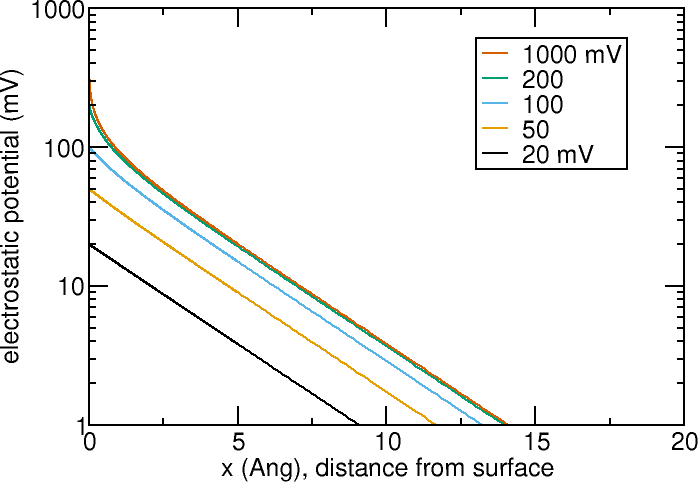
\includegraphics[width=0.45\linewidth]{counterion_potential.png}
(b)
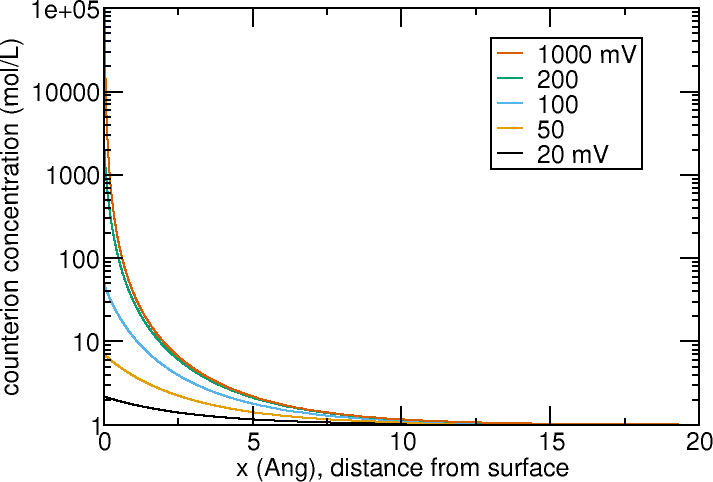
\includegraphics[width=0.45\linewidth]{counterion_logzero.png}
\caption{\label{fig_classical_PB}Solutions to the classical point
  charge Poisson-Boltzmann model of 1M NaCl electrolyte solution,
  shown as profiles along $x$, the perpendicular distance from an
  electrode surface (a) Electrostatic potential. (b) Counterion
  (\ce{Cl-}) concentration. }
\end{figure}

At still higher potentials the stability of simple log scaling with
respect to the coion must be considered. The coion, with same charge
as the electrostatic potential, is repelled from the electrode surface
with coion concentration trending towards zero at the electrode. At
sufficiently high potentials this generates values in the log-scaled
function that tend towards $-\infty$, which destabilises the numerical
solution. We therefore introduce a more complex log-scaling function,
\begin{equation}
Z_i(x) = \ln\left[c_i(x)/c_{i\infty}+1\right]/\ln 2 - 1
\label{log_zero}
\end{equation}
which keeps the scaled coion function constrained between -1 and 0
rather than $-\infty$ and 0. Since this scaling function addresses the
near-zero concentration of the coion, we call it ``log-zero'' scaling.

\section{Throttling algorithm}

Log-scaling of concentration functions makes a numerical solution to
the conventional Poisson-Boltzmann available at electrode potentials
up to 1.5V. Nevertheless \figref{fig_classical_PB}b demonstrates the
point charge catastrophe of the conventional model, with counterion
concentrations exceeding $10^{5}$ mol/L at the electrode
surface. Moreover, for general electrochemical applications it would
be desirable to be capable of obtaining solutions for electrode
potentials higher than 1.5V. To deal with the physical problem, we
introduce finite ion sizes with a steric force provided by the
Carnahan-Starling model, \eqnref{chem_pot_CS} (weak form
\eqnref{weak_CS}).  We apply ion volumes
$v_{\ce{Na}}=1.24 \text{\AA}^{3}$ per \ce{Na+} ion,
$v_{\ce{Cl}}=35.9 \text{\AA}^{3}$ per \ce{Cl-} ion (volumes taken from
quantum mechanical volumes of the ions' electron clouds
\cite{ParsonsNinham2009}).

The additional nonlinearity introduced by the Carnahan-Starling model,
where the chemical potential depends on the concentrations being
calculated, introduces a new challenge. The default nonlinear solver
in FEniCS assumes zero as an initial guess for the functions being
solved. But under the nonlinear conditions (with electrode potential
$>0.2$ V) where the Carnahan-Starling steric force is required, the
zero initial guess leads quickly to a diverging solution with infinite
residual. And yet a stable solution is accessible at lower values of
the boundary condition. We nudge the solver to a stable solution by
applying a throttling algorithm: reduce the boundary condition to a
small value for which a solution can be obtained, then incrementally
increase the boundary value back towards the target value, using the
previous found solution as an initial guess for the next
iteration. The approach is known to mathematicians as the homotopy
analysis method \cite{homotopy_analysis_Liao2012}, with our throttle
serving as a homotopy parameter applied to boundary conditions.
A flowchart for the algorithm is
shown in \figref{fig_throttling_algorithm}.

\begin{figure}
\centering
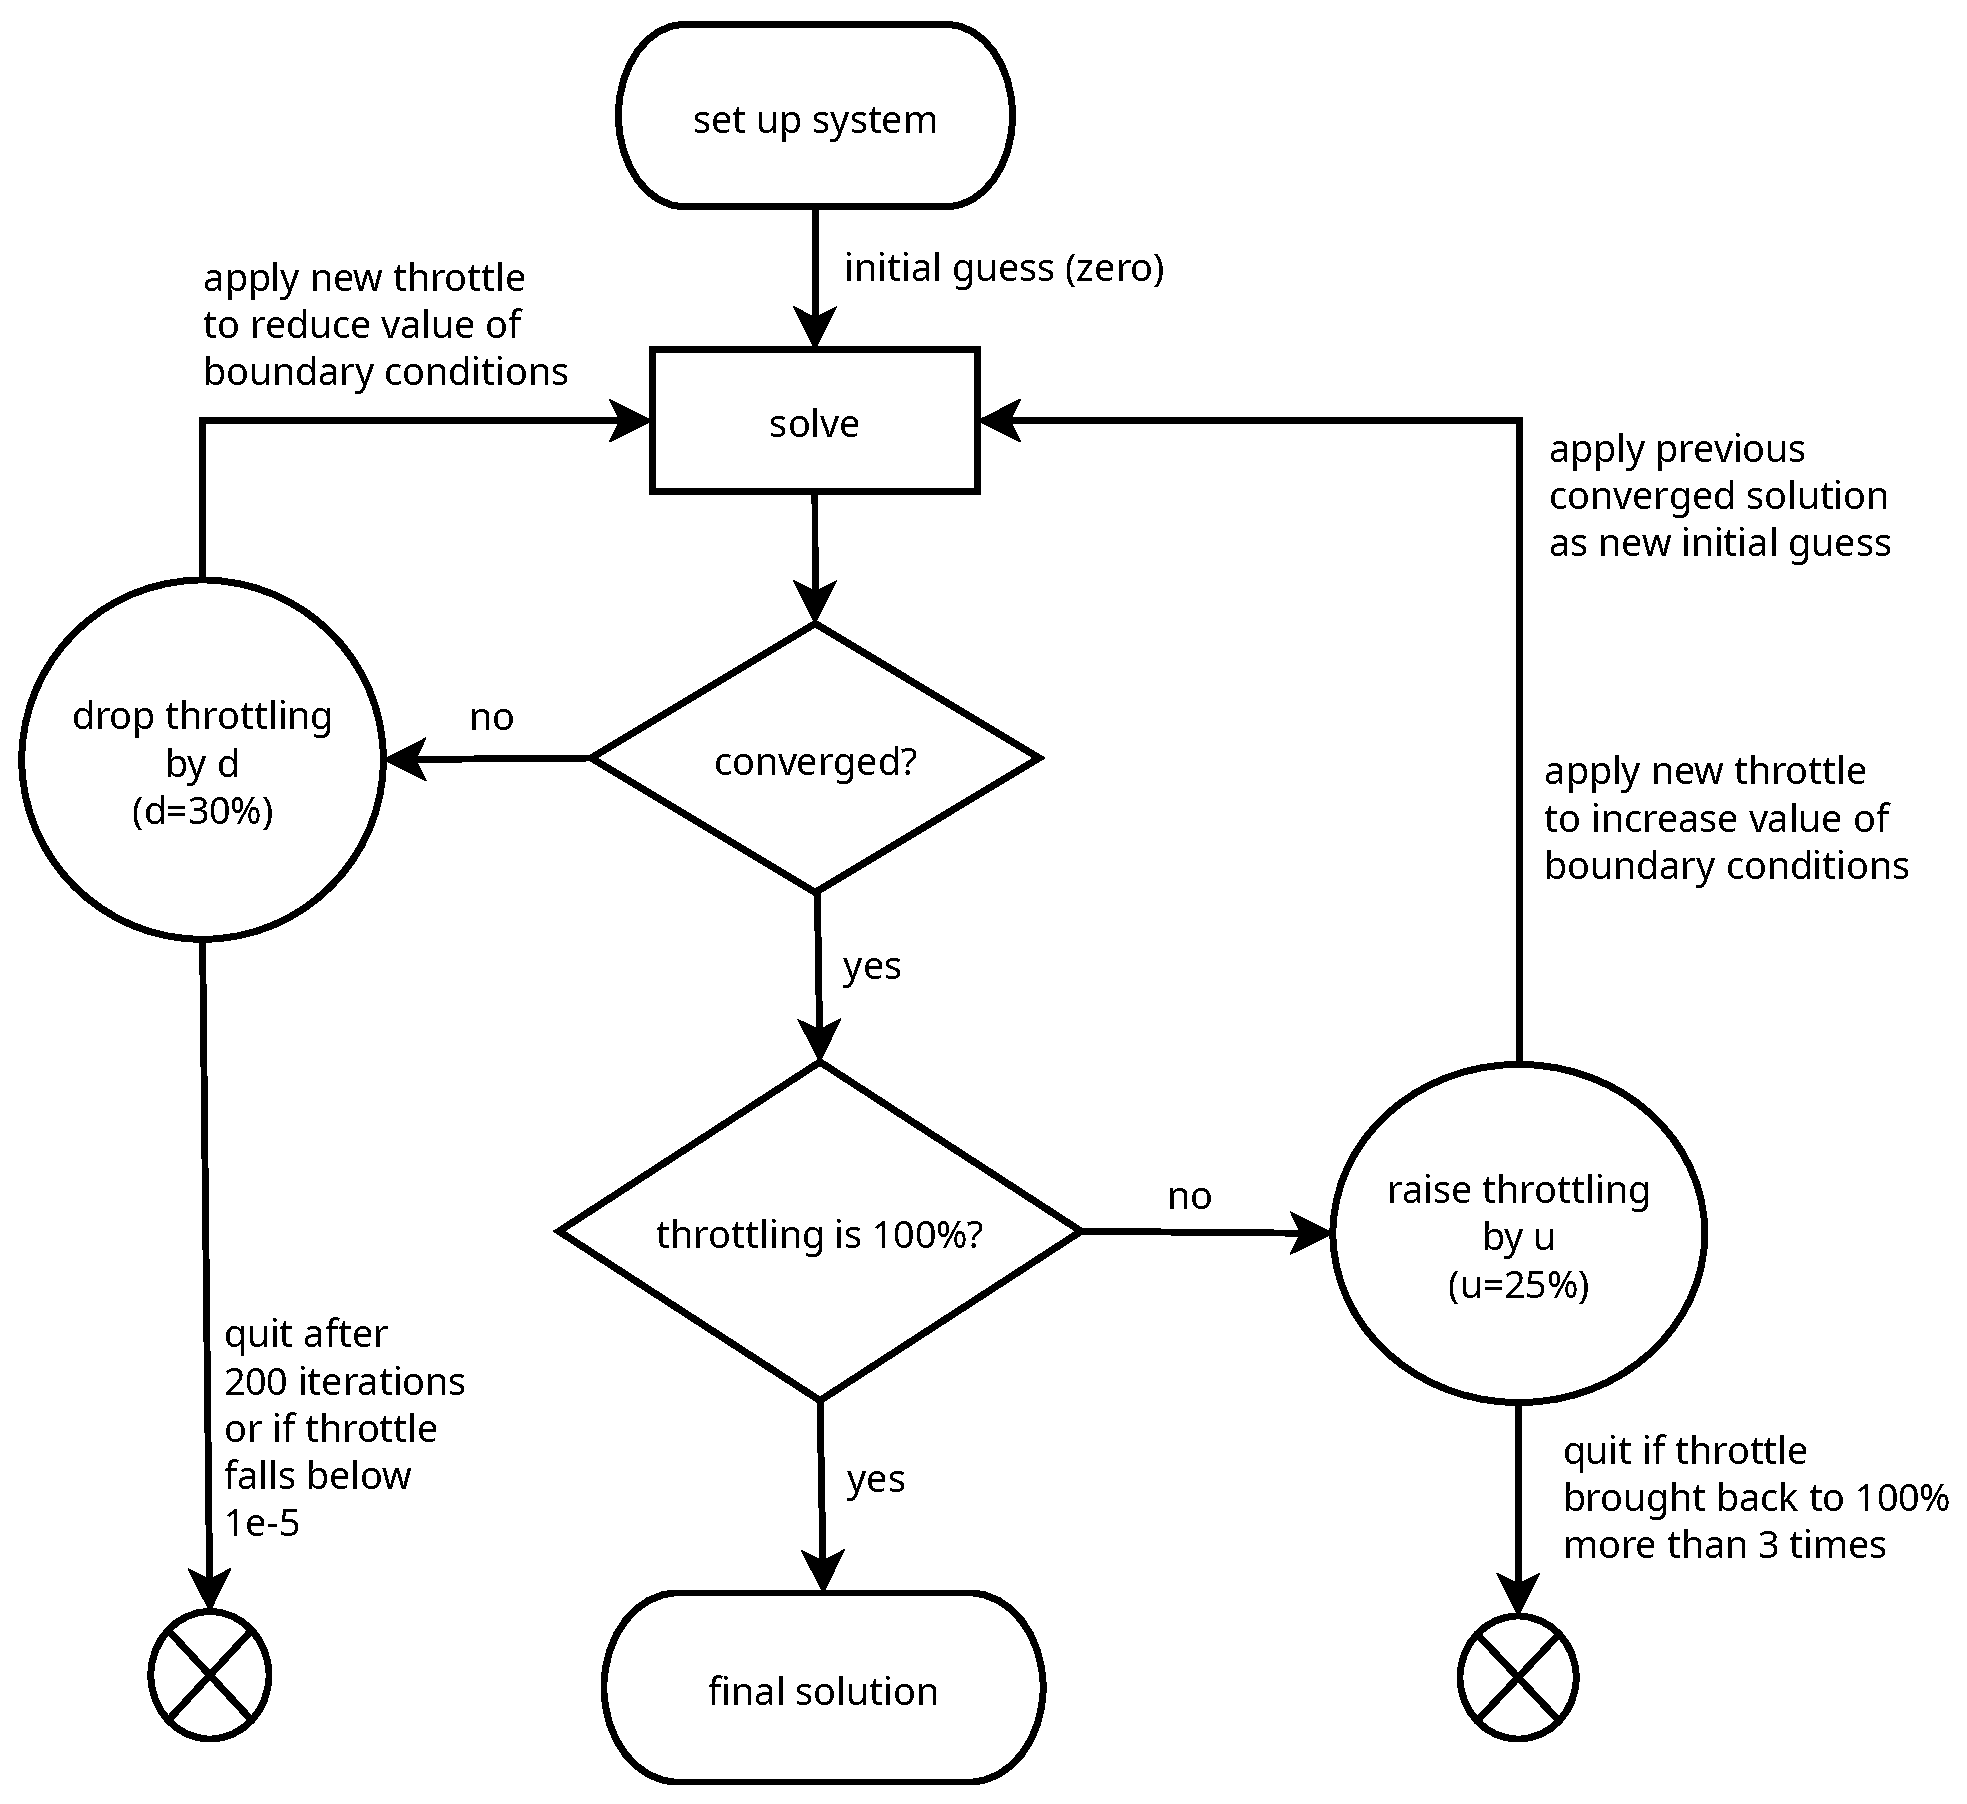
\includegraphics[width=0.8\linewidth]{throttling.eps}
\caption{\label{fig_throttling_algorithm}Flowchart for the throttling algorithm. }
\end{figure}

If the solver fails to converge, then reduce the throttle downwards to
a fraction $d$ of its previous value. The throttle is a multiplier
applied to the value of boundary conditions.  Once the boundary
condition is throttled enough to generate a converged solution, raise
the throttle upwards by an amount $u$, towards 100\% (set the throttle
to 100\% if the procedure would exceed it).  The values of $d$ and $u$
must find a balance between reaching 100\% throttle in as few
iterations as possible, while not collapsing back to non-converging
conditions when raising the throttle.  For potentials below 5V, we
find a drop level $d=75\%$ and a raise level $u=25\%$ with simple log
scaling of concentrations gives a reasonable balance between speed and
stability. If log-zero scaling is employed and the rise rate is
weakened to $u=10\%$, then electrode potentials of 20V can be
reached. With 5\% rising steps, 100V can be obtained. For a 1M
electrolyte, calculation at 240V would require such a small rise rate
that this algorithm becomes impractical.

If the throttling rates are not appropriately set, then the algorithm
may loop indefinitely between a converged solution at lower throttling
rate and non-convergence at a higher throttling rate. We therefore
halt after 200 throttle drops, or when the throttling rate drops below
$10^{-5}$, or when 100\% throttle is attempted more than 3 times.

The results of the throttling algorithm for an electrode charged to
10V, with Carnahan-Starling steric forces, is shown in
\figref{fig_results_throttling}. This solution was obtained with a
throttling rise rate of 10\% (0.1) and log-zero scaling of the
concentration functions
(\eqnref{log_zero}). \figref{fig_results_throttling} shows the onset
of a steric adsorption layer \cite{DagmawiParsons2022} with counterion
concentrations constrained below a concentration cap determined by the
ion size.

\begin{figure}
\centering
(a)
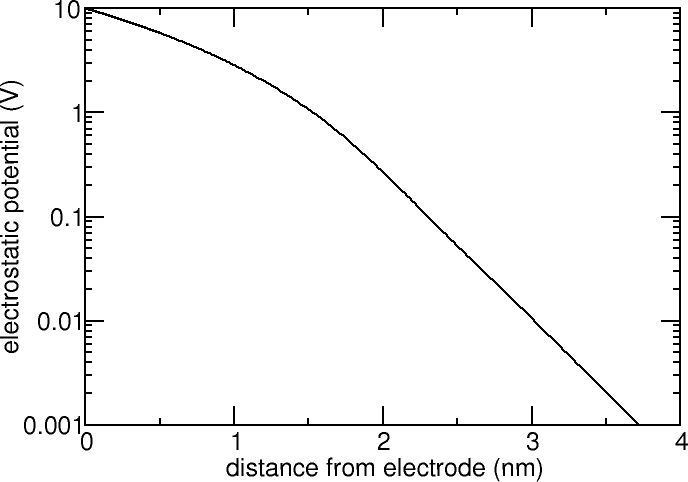
\includegraphics[width=0.4\linewidth]{steric_potential_10V.png}
(b)
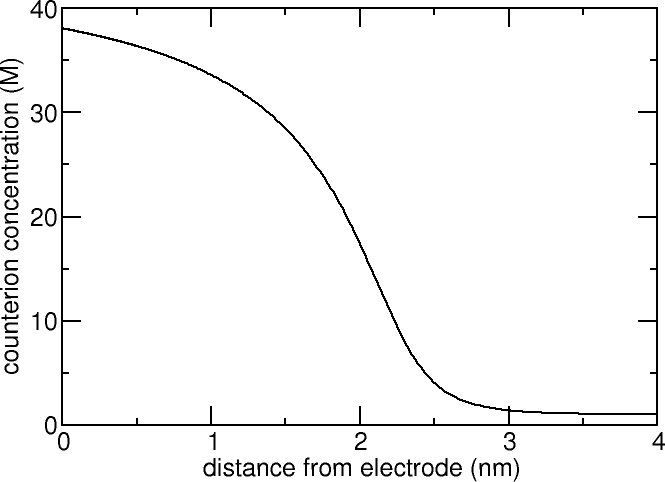
\includegraphics[width=0.4\linewidth]{steric_10V_counterion.png}
\caption{\label{fig_results_throttling}Solutions to the modified
  Poisson-Boltzmann model of a 1M NaCl electrolyte solution with
  Carnahan-Starling steric forces, shown as profiles along $x$, the
  perpendicular distance from a 5V electrode surface (a) Electrostatic
  potential. (b) Counterion (\ce{Cl-}) concentration. }
\end{figure}

\figref{fig_all_potential_high} presents algorithm conditions required
to obtains solutions (electrostatic potential profiles) up to
100V. Linear scaling (yellow region) is successful only for
$V<0.5$V. Log-scaling, \eqnref{log_scaling}, (purple region) with
throttling rise rate 25\% is successful up to 5V (purple
region). Log-zero scaling, \eqnref{log_zero}, with throttling rise
rate 10\% functions up to $V<20$V (blue region). Log-zero scaling with
5\% throttling rise rate can access up to $V<100$V (green region).

\begin{figure}
\centering
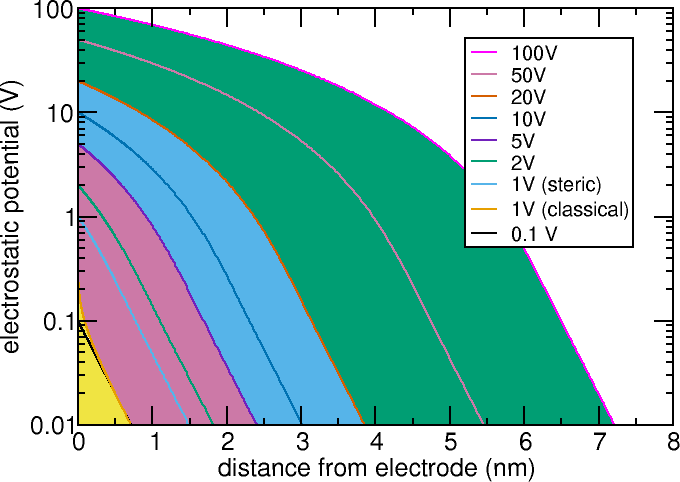
\includegraphics[width=0.9\linewidth]{counterion_potential_CS_bands.png}
\caption{\label{fig_all_potential_high} Algorithm conditions for
  electrostatic potential profiles with electrode potentials up to
  100V. Electrolyte is 1M NaCl. Linear scaling is functional for
  electrode potential $V<0.5$V (yellow region), log scaling (with
  steric forces) for $V<5$V with throttling rise rate 25\% (purple
  region), log-zero scaling with throttling rise rate 10\% for $V<20$V
  (blue region), and 5\% throttling rise rate for $V<100$V (green
  region).  }
\end{figure}

\section{Conclusion}

Modelling complex electrolyte solutions in electrochemical conditions
with electrode potentials 1V or greater requires both nontrivial
physics and nontrivial numerical algorithms. With respect to the
physics, aside from redox chemistry and electrolysis (not considered
here), the finite sizes of ions must be taken into consideration. With
respect to numerical convergence, we have proposed two
features. Firstly, we propose log-zero function scaling that accounts
not only for the heightened concentrations of counterions near an
electrode, but also the near-zero concentrations of coions. Secondly,
we propose a throttling algorithm that reduces boundary conditions
down to the linear regime where a solution is easily obtained, then
progressively propagating that solution by releasing the throttle
until the target boundary condition is obtained. The combination of
log-zero scaling and throttling enables calculations of electrolyte
solutions with electrode potentials up to 100V to be obtained. We
illustrated the throttling algorithm using Dirichlet boundary
conditions (electrode potentials), but the same principle applies
equally to Neumann or more complex boundary conditions.

\begin{acknowledgement}
  We acknowledge the award of CINECA support under the ISCRA
  initiative, for the availability of high-performance computing
  resources and support.
\end{acknowledgement}

\bibliographystyle{spbasic}
% Write the full path of your bibfile relative to book.tex
\bibliography{chapters/chp1/bibliography.bib}



% Write the full path to the location of the graphics relative to book.tex
\graphicspath{{chapters/chp1/graphics/}}

\title{Function scaling and throttling for convergence control in highly nonlinear Poisson-Boltzmann electrolyte models.}
\titlerunning{Function Scaling and Convergence Throttling}

\author{D.~F.~Parsons, M.~Farci,  A.~Grigoras, Dagmawi Tadesse}
\authorrunning{Parsons et al.}

\institute{D.~F.~Parsons \email{drew.parsons@unica.it}
  \and M.~Farci \and A.~Grigoras
  \at University of Cagliari,
Department of Chemical and Geological Sciences \& CSGI,
Cittadella Universitaria, S.S. 554 bivio Sestu,
09042 Monserrato (CA), Italy
\and Dagmawi Tadesse
\at Murdoch University,
Discipline of Physics, Chemistry and Mathematics, 90 South St, Murdoch 6150, West Australia
}

\maketitle

\abstract{ The nonlinear Poisson-Boltzmann model of electrolyte
  solutions combines the Poisson equation for electrostatic potentials
  with a Boltzmann equilibrium of mobile ion concentrations. The
  Boltzmann equation $c(x) = c_0 \exp[-q\psi(x)/kT]$ is highly
  nonlinear once the electrostatic potential exceeds several thermal
  energy ($kT$) units (i.e.\ when $\psi>0.1$ V). This introduces two
  related numerical challenges. Firstly, suitable convergence criteria
  for the concentration functions becomes variable, depending on the
  boundary potential. Secondly a controlled initial guess must be
  provided must be provided to avoid the FEM calculation diverging to
  NaN. We resolve the first by logarithmic scaling of the
  concentration function, as suggested by the exponential nature of
  the Boltzmann equation.  However a nontrivial complex logarithmic
  form is required in order to allow for the near-zero concentrations
  of coions, which would trigger numerical divergence in a trivial
  $\ln[c(x)]$ scaled function. The second challenge is resolved by
  iteratively with a throttling algorithm that suppresses large
  boundary conditions down to the linear regime, which is then applied
  as an initial guess for the nonlinear regime. Our implementation
  allows for other nonelectrostatic molecular interactions important
  for modelling real chemical and electrochemical systems, in
  particular steric forces due to finite ions sizes, enabling
  computation of concentrated electrolytes with electrode potentials
  as high as 100V.  }

\section*{Introduction}

Continuum theory (mean field theory) has been an effective tool for
studying the behaviour of systems in electrolyte solutions. The
Poisson-Boltzmann (PB) model \cite{Wu2022} enables evaluation of ion
adsorption layers at surfaces together with the electric field that
surface charge and adsorbed ions generate. Its nonequilibrium
counterpart, the Poisson-Nernst-Planck model
\cite{LopezGarciaHornoGrosse2018} (also called drift-diffusion)
likewise enables simulation of systems under conditions of moving
current. The PB model underpins theory of colloidal stability,
enabling modelling of nanoparticle aggregation and surface forces. The
same theory can in principle be applied to model electrochemical
systems, including energy storage devices, batteries or
supercapacitors. But there is a crucial difference in the two classes
of application, which has a significant impact on the numerical
stability of the model.  The surface potentials (or zeta potentials)
of typical colloidal systems such as protein molecules or metal oxide
particles tends to be found in the range 5--50 mV, which is 0.2--2
$kT$ in thermal energy units (based on a thermal potential at $T=298$
K defined by $e\psi_{T} = kT$ (where $e$ is the elementary charge, $k$
is Boltzmann's constant, $T$ is temperature). Electrolytic energy
storage systems, by contrast, typically operate with electrode
potentials of the order of 1--5 V, that is 1000--5000 mV, or 40--200
$kT$.  The nonlinearity of the Poisson-Boltzmann model is highly
sensitive to energies exceeding one $kT$ unit, requiring particular
algorithms to enable numerical nonlinear convergence.  Our goal is to
set up the calculation to solve successfully over a broad range of
electrode potentials without requiring manual readjustment of
convergence parameters.  We identify two main steps, implemented via
finite element methods (using FEniCSx\cite{baratta2023dolfinx}): log-scaling of
ion concentration functions, and throttling of boundary
conditions. For context we also present a summary of the physics and
weak formulation defining the Poisson-Boltzmann model, including
finite ion size effects. For simplicity we omit redox phenomenon
(electrolysis of water would occur in real systems at high electrode
potentials).

\section{Weak formulation of the Poisson-Boltzmann model}

The energy functional for an electrolyte solution, determined by
electrostatic potential $\psi(x)$ and ion concentration profiles
$c_i(x)$, may be composed from various fundamental energy
contributions as
\begin{equation}
    \Omega[\psi, c_i] = \Omega_{el} + \Omega_{en} +  \Omega_{ex}
\end{equation}
$\Omega_{el}$ describes the direct energy of the electrostatic field generated by the electric charge of ions and surfaces, \cite{Jackson}
\begin{equation}
  \Omega_{el}  =\frac{1}{2} \int_{V}D \cdot E dx
  = -\frac{1}{2} \int_{V}D \cdot E dx + \sum_i \int_V z_i e c_i(x) \psi(x) dx
  + \int_{S} \sigma(s) \psi(s) ds
\end{equation}
where $E$ is the electric field $E=-\nabla\psi$ and $D$ is the
electric displacement $D=\varepsilon_0
\varepsilon(x)E$. $\varepsilon_0$ is the permittivity of the vacuum,
and $\varepsilon(x)$ is the (spatially varying) relative
permittivity. $z_i$ is the valency of ion $i$.  $\sigma(s)$ is the
surface charge density on boundary $S$.

$\Omega_{en}$ describes the ideal entropic energy of ions, treated as ideal (noninteracting) particles \cite{GrayStiles2018,DagmawiParsons2024},
\begin{equation}
    \Omega_{en} = kT \sum_{i} \int_{V} \left[ c_i(x) \ln \left(\frac{c_i(x)}{c_{i\infty}} \right) - c_{i}(x) + c_{i\infty} \right] dx 
\end{equation}
where $c_{i\infty}$ is the bulk concentration of ions. As a point of
physics it is important to note that the use of a fixed bulk
concentration means the system is controlled by the chemical potential
of ions with a variable number of ions in the domain $V$ of interest.
That is, the thermodynamic potential is a grand potential, not a
(Helmholtz) free energy (hence we write the energy as $\Omega$ rather
than $F$). A free energy formulation (with fixed number of ions) would
require use of a thermal de Broglie wavelength instead of
$c_{i\infty}$ \cite{GrayStiles2018}.

$\Omega_{el} + \Omega_{en}$ alone construct the conventional
Poisson-Boltzmann model. The term $\Omega_{ex}$ represents extra
contributions to the total energy functional that describes other
relevant physics, such as pH-dependent charge regulation
\cite{ParsonsSalis2019}, specific ion interactions
\cite{ParsonsCarucciSalis2022}, or steric forces due to finite ion
size \cite{LopezGarciaHornoGrosse2018}. We consider the latter in this
work.

The Poisson-Boltzmann model describes the system in equilibrium,
obtained by minimising the total grand potential with variation
$\delta\Omega=0$ with respect to $\psi$ and $c_i$. Variation with
respect to $\psi$ (with test function $p$) leads to a weak formulation
for the Poisson equation,
\begin{equation}
    0 = -\int_{V} \varepsilon_{0}\varepsilon(x) (\nabla\psi,\nabla p) dx + \sum_{i}z_i e \int_{V} c_{i}(x) p dx + \int_{S} \sigma(s) p ds  
    \label{weak_Poisson}
\end{equation}
for all $p$ in the relevant finite element space.  After additional
integration by parts, this weak formulation leads to the strong
formulation of the electrostatic Poisson equation,
$\nabla\cdot D = \sum_i z_i e c_{i}(x)$. Variation $\delta\Omega$ with
respect to each ion concentration profile $c_i$ (in turn, with test
function $b_i$), assuming linear variations with
$\ln(1+b_i/c_i)=b_i/c_i$, leads to the weak formulation of Boltzmann's
equation,
\begin{equation}
    0 = \int_{V}z_i e \psi(x) b_i dx
    + kT \int_{V} b_i \ln\left(\frac{c_i(x)}{c_{i\infty}}\right)dx
    \label{weak_Boltzmann}
\end{equation}
for all $b_i$. The strong form of the classical Boltzmann equation can then obtained, $c_i(x)=c_{i\infty}\exp(-z_i e \psi(x)/kT)$. 

It might be noted that in the classical Poisson-Boltzmann model, the
ion concentrations $c_i$ are determined completely by the
electrostatic potential with the Boltzmann equation in closed form, so
only the Poisson equation needs solving directly. However, the
physical problem with the classical model is evident in electrochemical
systems with electrode potential 1 V. A one volt potential is
equivalent to a thermal energy of $40 kT)$, for which the conventional
Boltzmann factor for a counterion is
$\exp(40)\approx 2.3 \times 10^{17}$.  That is, the surface counterion
concentration of a 1M electrolyte would exceed $10^{17}$ mol/L, which
is obviously unphysical.  We return the model back to physical
relevance by adding an extra steric energy term $\Omega_{ex}$ with
corresponding excess chemical potential per ion $\mu_{i}^{ex}$, for
which the modified Boltzmann equation is
\begin{equation}
    c_i(x)=c_{i\infty}\exp\left[(-(z_i e \psi(x) + \mu_i^{ex}(x)-\mu_{i\infty}^{ex})/kT\right]
    \label{general_Boltzmann}
\end{equation}
$\mu_{i\infty}$ refers to the (fixed) excess chemical potential of the ion in bulk solution.
The steric model we employ is the Carnahan-Starling model \cite{CarnahanStarling1969} with grand potential
\begin{equation}
    \Omega_{ex} = \sum_{i} \int_{V} c_{i}(x) \left[ kT
    \frac{4\phi - 3\phi^2}{(1-\phi)^2}
    -  \mu_{\infty}
    \right]dx
\end{equation}
and weak formulation
\begin{equation}
    0 = \int_{V} (\mu_i^{ex}-\mu_{i\infty}^{ex}) b_i
    \label{weak_CS}
\end{equation}
for all $b_i$, which adds to \eqnref{weak_Boltzmann}, the weak
formulation for the Boltzmann equation, together generating the strong
formulation of \eqnref{general_Boltzmann}, the modified Boltzmann
equation.  Here we have introduced from the excess chemical potential
per ion for the Carnahan-Starling model,
\begin{equation}
    \mu_{i}^{ex} = kT \frac{\phi(8-9\phi+3\phi^2)}{(1-\phi)^3}
    \label{chem_pot_CS}
\end{equation}
Crucially, $\phi$ is the \emph{total} ion volume fraction defined by
$\phi=\sum_i c_i v_i$ where $v_i$ is the intrinsic molar volume per
ion $i$. Hence the CS excess chemical potential is defined identically
for all ions. To derive the weak formulation in \eqnref{weak_CS}, we
applied an homogenised component approximation that assigns common
volumes when introducing the test function $b_i$ (which is the
variation $\delta c_i$), such that $\delta\phi=v_j \delta c_i$ rather
than $v_i \delta c_i$. This approximation is required since the CS
model was formulated for single component systems. The more complex
multicomponent BMCSL model would enable ion specific chemical
potentials \cite{MansooriCarnahanStarlingLeland1971}, removing the
need for this approximation.  $\phi_{\infty}$, $\mu_{i\infty}^{ex}$
are the bulk total volume fraction and excess chemical potential
defined by bulk concentrations $c_{i\infty}$. With this term, the
Boltzmann equation is transcendental in $c_i$, precluding a closed
expression determining ion concentrations, which must therefore be
explicitly numerically solved alongside potential $\psi$. In this
paper we address strategies for managing the strong nonlinearity in
the system introduced by this term alongside large values of the
potential. Note that $c_i$ must also be solved explicitly in the case
of time-dependent nonequilibrium Poisson-Nernst-Planck systems where
ion concentrations are not in equilibrium and determined by a
continuity equation rather than a Boltzmann equation.

\section{Function scaling}
We constructed a finite element implementation of the weak
formulation(\eqnref{weak_Poisson} and \ref{weak_Boltzmann} (and
\eqnref{weak_CS}) in FEniCS-X \cite{baratta2023dolfinx}, using continuous
Lagrange elements with polynomial order 2.  The electrolyte solution
is taken as NaCl with bulk concentration 1 mol/L.  To illustrate
general issues of nonlinear convergence, we calculate the
electrostatic and ion concentration profiles of ion adsorbed at a
single flat electrode surface along the direction perpendicular to the
surface, with the electrode boundary at $x=0$.  The electrode
potential is controlled (Dirichlet boundary condition), and bulk
solution represented by a zero Neumann condition ("zero electric
field") at a distance of 30 Debye lengths (at $x=9.1$ nm, for the 1M
electrolyte). Nonlinear solutions are computed using FEniCS-X's
NonlinearProblem with a standard NewtonSolver. Convergence criterion
is set to FEniCS-X's default "incremental" method with absolute
tolerance $10^{-5}$.

We must consider scaling of the concentration functions $c_i(x)$. We
already noted that the counterion concentration becomes unphysically
large in the conventional Poisson-Boltzmann model due to nonlinear
exponentiation of the electrostatic potentials exceeding 0.1--0.2 V in
the Boltzmann equation. Trivial scaling may be introduced by solving
the concentration function scaled against the bulk concentration. But
with a convergence criterion of the nonlinear catastrophe is reached
numerically above 0.5 V. Already at 0.6 V, the conventional
calculation with simple scaling is unable to reduce the residual below
the required $10^{-5}$. While it would be possible to relax the
convergence tolerance to obtain a reasonable solution, our aim is to
obtain a robust general solver not requiring close manipulation of
convergence criteria. For instance, one application is modelling the
cyclic voltammetry curve of an electrode which require calculations
over a potential window as wide as $-5$ to 5 V.

The challenge arises due to the extreme magnitudes of the counterion
concentration at the electrode surface. The weak formulation for the
Boltzmann equation in \eqnref{weak_Boltzmann} suggests a solution:
solve for the concentration function in log-form,
\begin{equation}
C_{i}(x) = \ln[ c_{i}(x) / c_{i\infty}]
\label{log_scaling}
\end{equation}
rather than the concentration function $c_{i}(x)$ directly. Log
scaling extends the solvability of the conventional Poisson-Boltzmann
model up to electrode potentials as high as 1.5 V. Solutions for the
electrostatic potential and counterion concentration profile are shown
in \figref{fig_classical_PB}. Shown on a log scale, strong
nonlinearity in the PB system becomes apparent in the bend in the
electrostatic potential (\figref{fig_classical_PB}a) close to the
surface where $x<2$\AA for electrode potentials $> 0.2$ V.


\begin{figure}
\centering
(a)
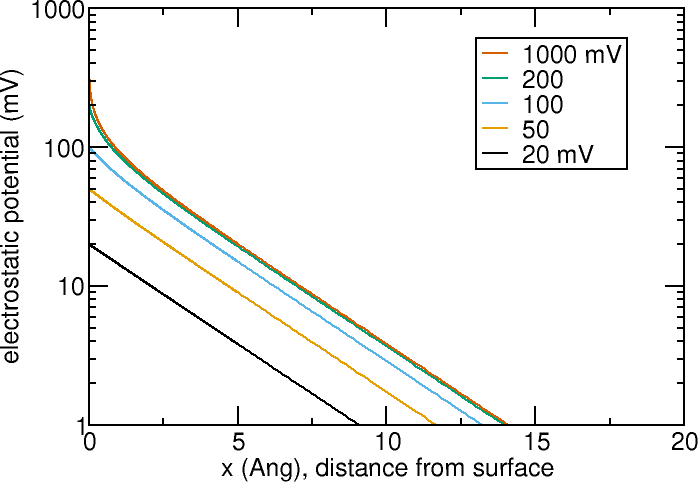
\includegraphics[width=0.45\linewidth]{counterion_potential.png}
(b)
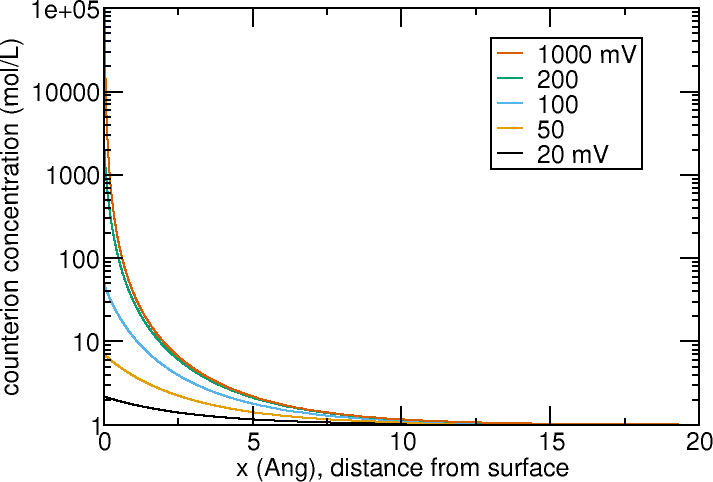
\includegraphics[width=0.45\linewidth]{counterion_logzero.png}
\caption{\label{fig_classical_PB}Solutions to the classical point
  charge Poisson-Boltzmann model of 1M NaCl electrolyte solution,
  shown as profiles along $x$, the perpendicular distance from an
  electrode surface (a) Electrostatic potential. (b) Counterion
  (\ce{Cl-}) concentration. }
\end{figure}

At still higher potentials the stability of simple log scaling with
respect to the coion must be considered. The coion, with same charge
as the electrostatic potential, is repelled from the electrode surface
with coion concentration trending towards zero at the electrode. At
sufficiently high potentials this generates values in the log-scaled
function that tend towards $-\infty$, which destabilises the numerical
solution. We therefore introduce a more complex log-scaling function,
\begin{equation}
Z_i(x) = \ln\left[c_i(x)/c_{i\infty}+1\right]/\ln 2 - 1
\label{log_zero}
\end{equation}
which keeps the scaled coion function constrained between -1 and 0
rather than $-\infty$ and 0. Since this scaling function addresses the
near-zero concentration of the coion, we call it ``log-zero'' scaling.

\section{Throttling algorithm}

Log-scaling of concentration functions makes a numerical solution to
the conventional Poisson-Boltzmann available at electrode potentials
up to 1.5V. Nevertheless \figref{fig_classical_PB}b demonstrates the
point charge catastrophe of the conventional model, with counterion
concentrations exceeding $10^{5}$ mol/L at the electrode
surface. Moreover, for general electrochemical applications it would
be desirable to be capable of obtaining solutions for electrode
potentials higher than 1.5V. To deal with the physical problem, we
introduce finite ion sizes with a steric force provided by the
Carnahan-Starling model, \eqnref{chem_pot_CS} (weak form
\eqnref{weak_CS}).  We apply ion volumes
$v_{\ce{Na}}=1.24 \text{\AA}^{3}$ per \ce{Na+} ion,
$v_{\ce{Cl}}=35.9 \text{\AA}^{3}$ per \ce{Cl-} ion (volumes taken from
quantum mechanical volumes of the ions' electron clouds
\cite{ParsonsNinham2009}).

The additional nonlinearity introduced by the Carnahan-Starling model,
where the chemical potential depends on the concentrations being
calculated, introduces a new challenge. The default nonlinear solver
in FEniCS assumes zero as an initial guess for the functions being
solved. But under the nonlinear conditions (with electrode potential
$>0.2$ V) where the Carnahan-Starling steric force is required, the
zero initial guess leads quickly to a diverging solution with infinite
residual. And yet a stable solution is accessible at lower values of
the boundary condition. We nudge the solver to a stable solution by
applying a throttling algorithm: reduce the boundary condition to a
small value for which a solution can be obtained, then incrementally
increase the boundary value back towards the target value, using the
previous found solution as an initial guess for the next
iteration. The approach is known to mathematicians as the homotopy
analysis method \cite{homotopy_analysis_Liao2012}, with our throttle
serving as a homotopy parameter applied to boundary conditions.
A flowchart for the algorithm is
shown in \figref{fig_throttling_algorithm}.

\begin{figure}
\centering
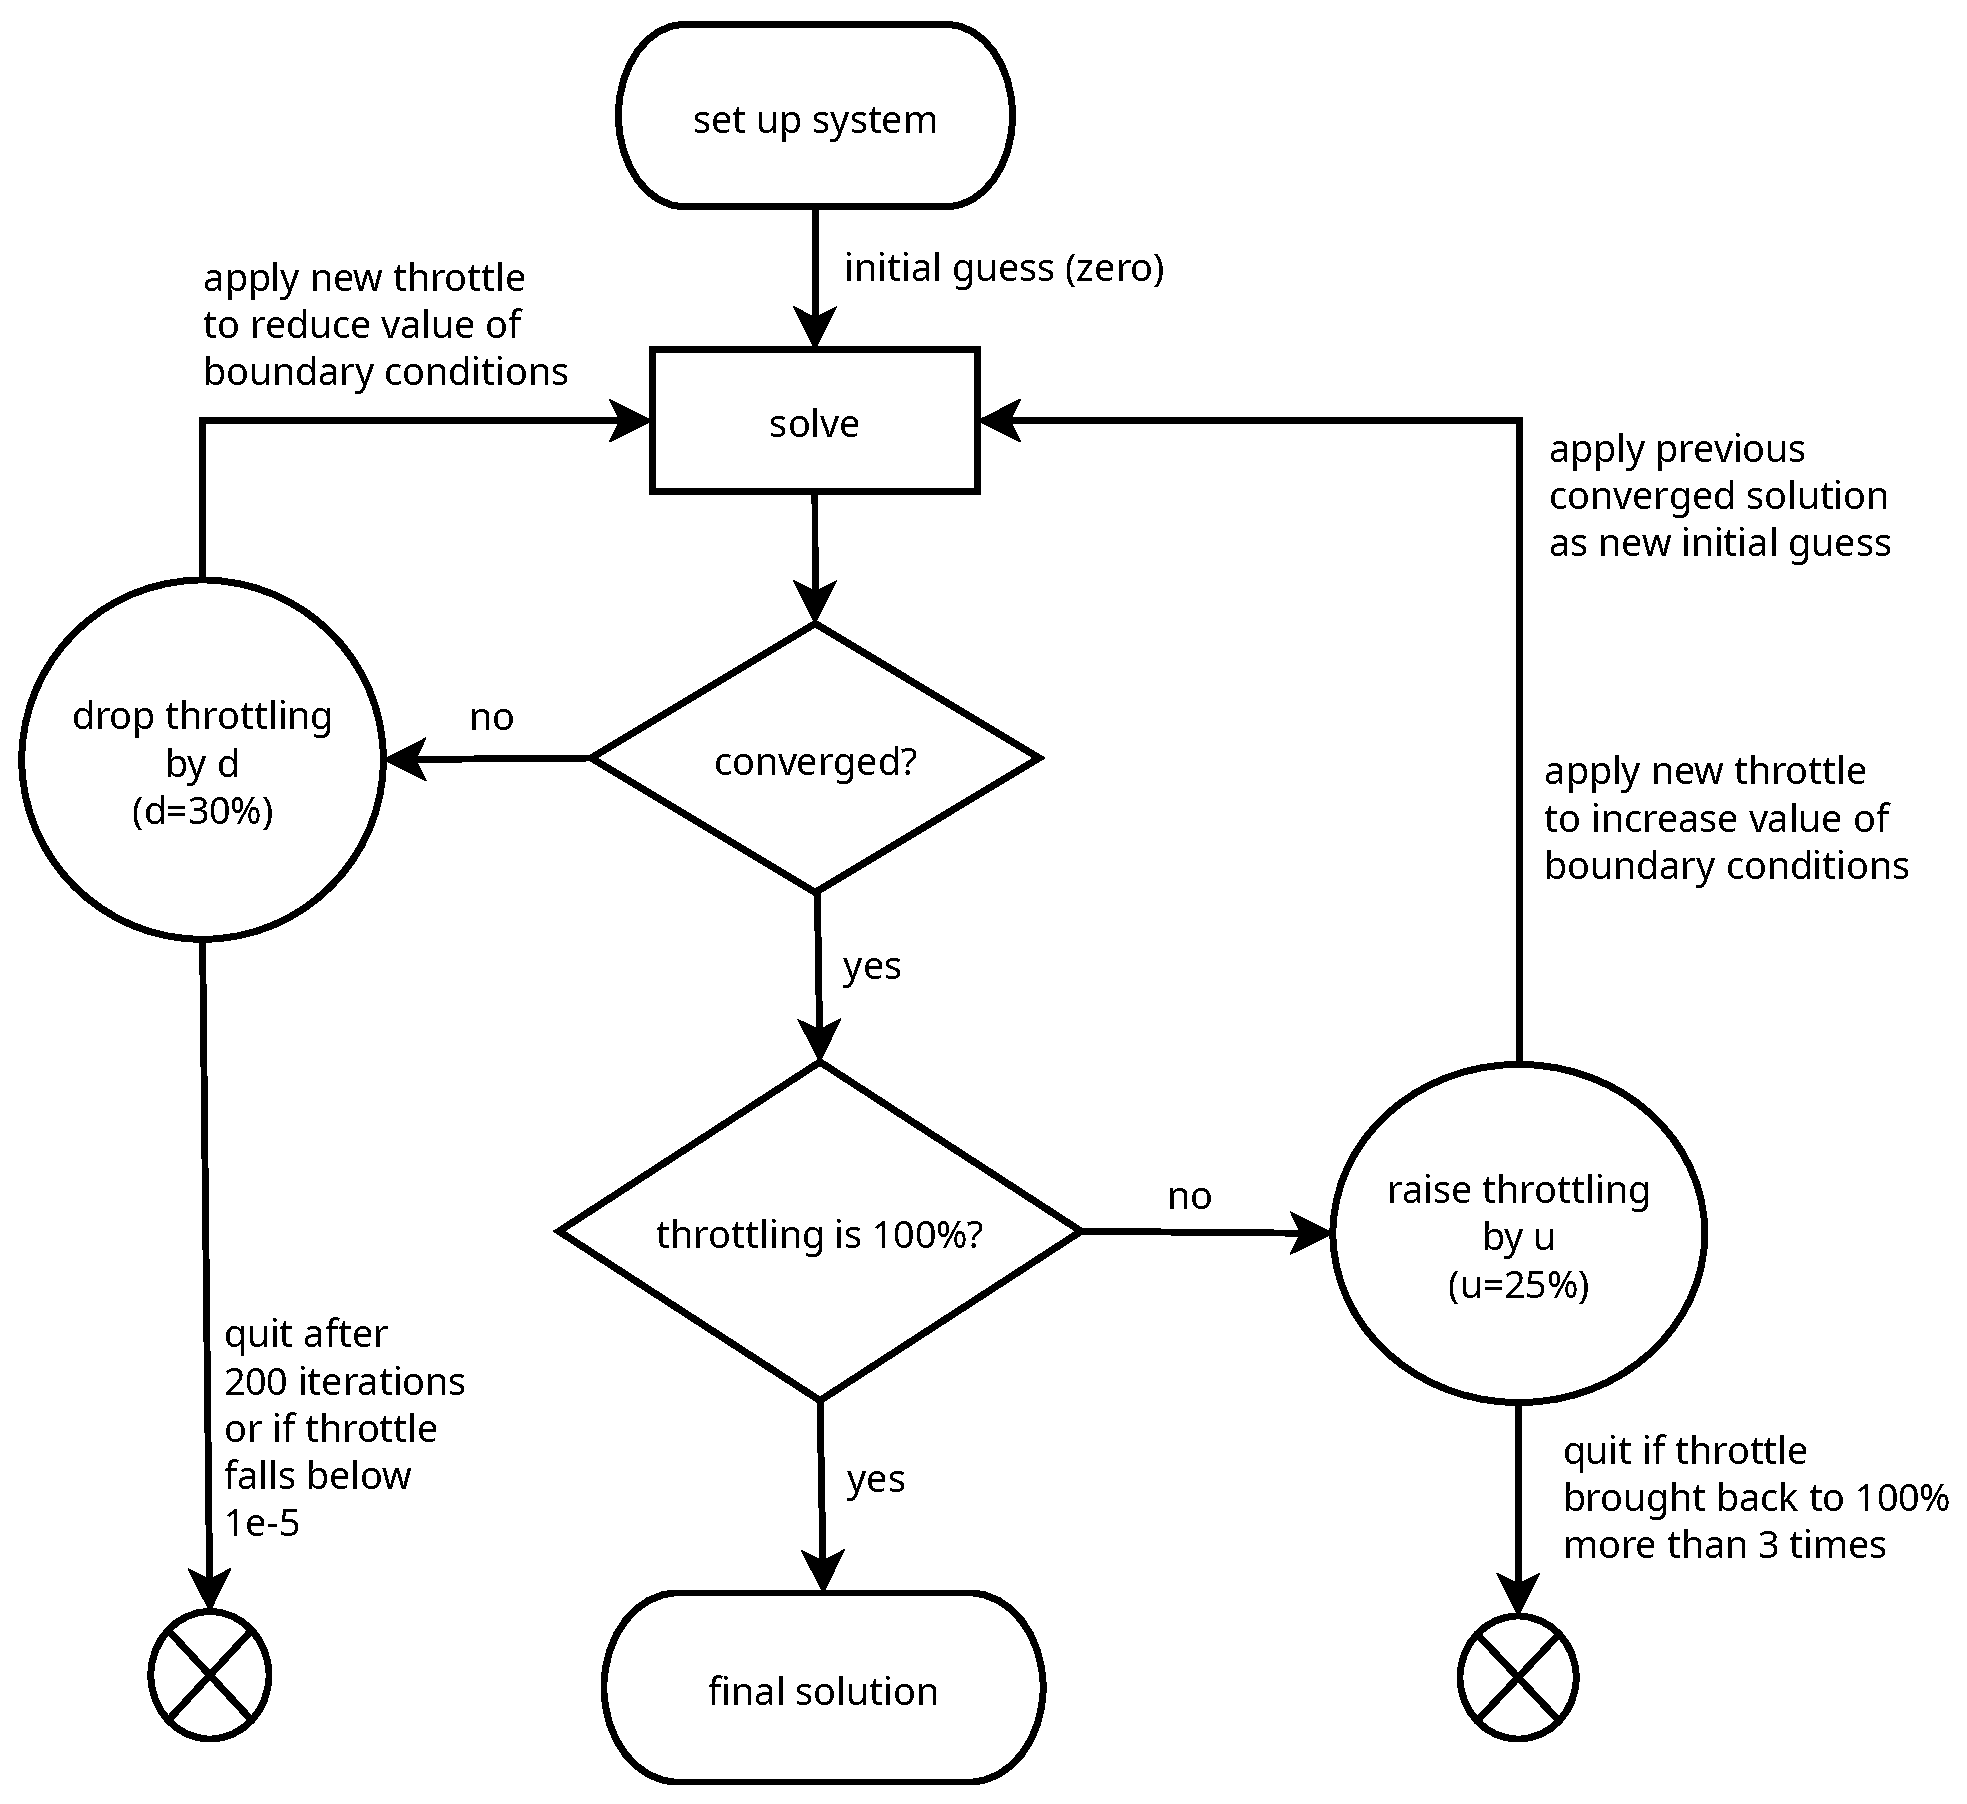
\includegraphics[width=0.8\linewidth]{throttling.eps}
\caption{\label{fig_throttling_algorithm}Flowchart for the throttling algorithm. }
\end{figure}

If the solver fails to converge, then reduce the throttle downwards to
a fraction $d$ of its previous value. The throttle is a multiplier
applied to the value of boundary conditions.  Once the boundary
condition is throttled enough to generate a converged solution, raise
the throttle upwards by an amount $u$, towards 100\% (set the throttle
to 100\% if the procedure would exceed it).  The values of $d$ and $u$
must find a balance between reaching 100\% throttle in as few
iterations as possible, while not collapsing back to non-converging
conditions when raising the throttle.  For potentials below 5V, we
find a drop level $d=75\%$ and a raise level $u=25\%$ with simple log
scaling of concentrations gives a reasonable balance between speed and
stability. If log-zero scaling is employed and the rise rate is
weakened to $u=10\%$, then electrode potentials of 20V can be
reached. With 5\% rising steps, 100V can be obtained. For a 1M
electrolyte, calculation at 240V would require such a small rise rate
that this algorithm becomes impractical.

If the throttling rates are not appropriately set, then the algorithm
may loop indefinitely between a converged solution at lower throttling
rate and non-convergence at a higher throttling rate. We therefore
halt after 200 throttle drops, or when the throttling rate drops below
$10^{-5}$, or when 100\% throttle is attempted more than 3 times.

The results of the throttling algorithm for an electrode charged to
10V, with Carnahan-Starling steric forces, is shown in
\figref{fig_results_throttling}. This solution was obtained with a
throttling rise rate of 10\% (0.1) and log-zero scaling of the
concentration functions
(\eqnref{log_zero}). \figref{fig_results_throttling} shows the onset
of a steric adsorption layer \cite{DagmawiParsons2022} with counterion
concentrations constrained below a concentration cap determined by the
ion size.

\begin{figure}
\centering
(a)
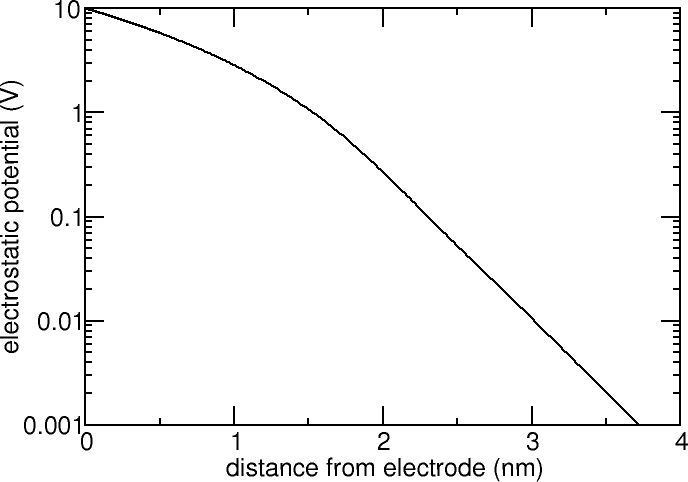
\includegraphics[width=0.4\linewidth]{steric_potential_10V.png}
(b)
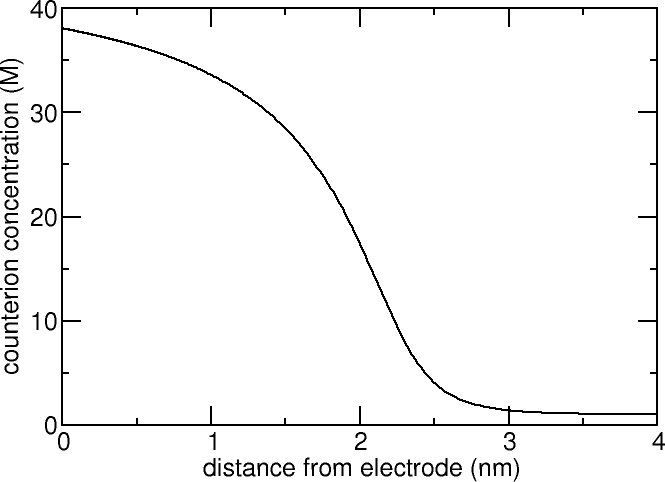
\includegraphics[width=0.4\linewidth]{steric_10V_counterion.png}
\caption{\label{fig_results_throttling}Solutions to the modified
  Poisson-Boltzmann model of a 1M NaCl electrolyte solution with
  Carnahan-Starling steric forces, shown as profiles along $x$, the
  perpendicular distance from a 5V electrode surface (a) Electrostatic
  potential. (b) Counterion (\ce{Cl-}) concentration. }
\end{figure}

\figref{fig_all_potential_high} presents algorithm conditions required
to obtains solutions (electrostatic potential profiles) up to
100V. Linear scaling (yellow region) is successful only for
$V<0.5$V. Log-scaling, \eqnref{log_scaling}, (purple region) with
throttling rise rate 25\% is successful up to 5V (purple
region). Log-zero scaling, \eqnref{log_zero}, with throttling rise
rate 10\% functions up to $V<20$V (blue region). Log-zero scaling with
5\% throttling rise rate can access up to $V<100$V (green region).

\begin{figure}
\centering
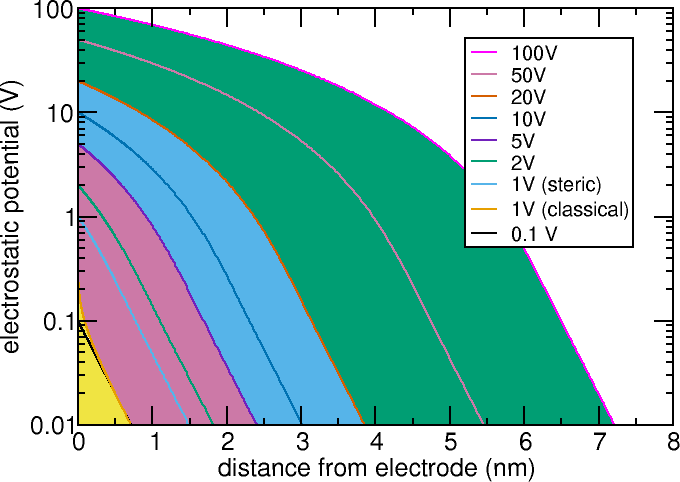
\includegraphics[width=0.9\linewidth]{counterion_potential_CS_bands.png}
\caption{\label{fig_all_potential_high} Algorithm conditions for
  electrostatic potential profiles with electrode potentials up to
  100V. Electrolyte is 1M NaCl. Linear scaling is functional for
  electrode potential $V<0.5$V (yellow region), log scaling (with
  steric forces) for $V<5$V with throttling rise rate 25\% (purple
  region), log-zero scaling with throttling rise rate 10\% for $V<20$V
  (blue region), and 5\% throttling rise rate for $V<100$V (green
  region).  }
\end{figure}

\section{Conclusion}

Modelling complex electrolyte solutions in electrochemical conditions
with electrode potentials 1V or greater requires both nontrivial
physics and nontrivial numerical algorithms. With respect to the
physics, aside from redox chemistry and electrolysis (not considered
here), the finite sizes of ions must be taken into consideration. With
respect to numerical convergence, we have proposed two
features. Firstly, we propose log-zero function scaling that accounts
not only for the heightened concentrations of counterions near an
electrode, but also the near-zero concentrations of coions. Secondly,
we propose a throttling algorithm that reduces boundary conditions
down to the linear regime where a solution is easily obtained, then
progressively propagating that solution by releasing the throttle
until the target boundary condition is obtained. The combination of
log-zero scaling and throttling enables calculations of electrolyte
solutions with electrode potentials up to 100V to be obtained. We
illustrated the throttling algorithm using Dirichlet boundary
conditions (electrode potentials), but the same principle applies
equally to Neumann or more complex boundary conditions.

\begin{acknowledgement}
  We acknowledge the award of CINECA support under the ISCRA
  initiative, for the availability of high-performance computing
  resources and support.
\end{acknowledgement}

\bibliographystyle{spbasic}
% Write the full path of your bibfile relative to book.tex
\bibliography{chapters/chp1/bibliography.bib}


 
% Write the full path to the location of the graphics relative to book.tex
\graphicspath{{chapters/chp1/graphics/}}

\title{Function scaling and throttling for convergence control in highly nonlinear Poisson-Boltzmann electrolyte models.}
\titlerunning{Function Scaling and Convergence Throttling}

\author{D.~F.~Parsons, M.~Farci,  A.~Grigoras, Dagmawi Tadesse}
\authorrunning{Parsons et al.}

\institute{D.~F.~Parsons \email{drew.parsons@unica.it}
  \and M.~Farci \and A.~Grigoras
  \at University of Cagliari,
Department of Chemical and Geological Sciences \& CSGI,
Cittadella Universitaria, S.S. 554 bivio Sestu,
09042 Monserrato (CA), Italy
\and Dagmawi Tadesse
\at Murdoch University,
Discipline of Physics, Chemistry and Mathematics, 90 South St, Murdoch 6150, West Australia
}

\maketitle

\abstract{ The nonlinear Poisson-Boltzmann model of electrolyte
  solutions combines the Poisson equation for electrostatic potentials
  with a Boltzmann equilibrium of mobile ion concentrations. The
  Boltzmann equation $c(x) = c_0 \exp[-q\psi(x)/kT]$ is highly
  nonlinear once the electrostatic potential exceeds several thermal
  energy ($kT$) units (i.e.\ when $\psi>0.1$ V). This introduces two
  related numerical challenges. Firstly, suitable convergence criteria
  for the concentration functions becomes variable, depending on the
  boundary potential. Secondly a controlled initial guess must be
  provided must be provided to avoid the FEM calculation diverging to
  NaN. We resolve the first by logarithmic scaling of the
  concentration function, as suggested by the exponential nature of
  the Boltzmann equation.  However a nontrivial complex logarithmic
  form is required in order to allow for the near-zero concentrations
  of coions, which would trigger numerical divergence in a trivial
  $\ln[c(x)]$ scaled function. The second challenge is resolved by
  iteratively with a throttling algorithm that suppresses large
  boundary conditions down to the linear regime, which is then applied
  as an initial guess for the nonlinear regime. Our implementation
  allows for other nonelectrostatic molecular interactions important
  for modelling real chemical and electrochemical systems, in
  particular steric forces due to finite ions sizes, enabling
  computation of concentrated electrolytes with electrode potentials
  as high as 100V.  }

\section*{Introduction}

Continuum theory (mean field theory) has been an effective tool for
studying the behaviour of systems in electrolyte solutions. The
Poisson-Boltzmann (PB) model \cite{Wu2022} enables evaluation of ion
adsorption layers at surfaces together with the electric field that
surface charge and adsorbed ions generate. Its nonequilibrium
counterpart, the Poisson-Nernst-Planck model
\cite{LopezGarciaHornoGrosse2018} (also called drift-diffusion)
likewise enables simulation of systems under conditions of moving
current. The PB model underpins theory of colloidal stability,
enabling modelling of nanoparticle aggregation and surface forces. The
same theory can in principle be applied to model electrochemical
systems, including energy storage devices, batteries or
supercapacitors. But there is a crucial difference in the two classes
of application, which has a significant impact on the numerical
stability of the model.  The surface potentials (or zeta potentials)
of typical colloidal systems such as protein molecules or metal oxide
particles tends to be found in the range 5--50 mV, which is 0.2--2
$kT$ in thermal energy units (based on a thermal potential at $T=298$
K defined by $e\psi_{T} = kT$ (where $e$ is the elementary charge, $k$
is Boltzmann's constant, $T$ is temperature). Electrolytic energy
storage systems, by contrast, typically operate with electrode
potentials of the order of 1--5 V, that is 1000--5000 mV, or 40--200
$kT$.  The nonlinearity of the Poisson-Boltzmann model is highly
sensitive to energies exceeding one $kT$ unit, requiring particular
algorithms to enable numerical nonlinear convergence.  Our goal is to
set up the calculation to solve successfully over a broad range of
electrode potentials without requiring manual readjustment of
convergence parameters.  We identify two main steps, implemented via
finite element methods (using FEniCSx\cite{baratta2023dolfinx}): log-scaling of
ion concentration functions, and throttling of boundary
conditions. For context we also present a summary of the physics and
weak formulation defining the Poisson-Boltzmann model, including
finite ion size effects. For simplicity we omit redox phenomenon
(electrolysis of water would occur in real systems at high electrode
potentials).

\section{Weak formulation of the Poisson-Boltzmann model}

The energy functional for an electrolyte solution, determined by
electrostatic potential $\psi(x)$ and ion concentration profiles
$c_i(x)$, may be composed from various fundamental energy
contributions as
\begin{equation}
    \Omega[\psi, c_i] = \Omega_{el} + \Omega_{en} +  \Omega_{ex}
\end{equation}
$\Omega_{el}$ describes the direct energy of the electrostatic field generated by the electric charge of ions and surfaces, \cite{Jackson}
\begin{equation}
  \Omega_{el}  =\frac{1}{2} \int_{V}D \cdot E dx
  = -\frac{1}{2} \int_{V}D \cdot E dx + \sum_i \int_V z_i e c_i(x) \psi(x) dx
  + \int_{S} \sigma(s) \psi(s) ds
\end{equation}
where $E$ is the electric field $E=-\nabla\psi$ and $D$ is the
electric displacement $D=\varepsilon_0
\varepsilon(x)E$. $\varepsilon_0$ is the permittivity of the vacuum,
and $\varepsilon(x)$ is the (spatially varying) relative
permittivity. $z_i$ is the valency of ion $i$.  $\sigma(s)$ is the
surface charge density on boundary $S$.

$\Omega_{en}$ describes the ideal entropic energy of ions, treated as ideal (noninteracting) particles \cite{GrayStiles2018,DagmawiParsons2024},
\begin{equation}
    \Omega_{en} = kT \sum_{i} \int_{V} \left[ c_i(x) \ln \left(\frac{c_i(x)}{c_{i\infty}} \right) - c_{i}(x) + c_{i\infty} \right] dx 
\end{equation}
where $c_{i\infty}$ is the bulk concentration of ions. As a point of
physics it is important to note that the use of a fixed bulk
concentration means the system is controlled by the chemical potential
of ions with a variable number of ions in the domain $V$ of interest.
That is, the thermodynamic potential is a grand potential, not a
(Helmholtz) free energy (hence we write the energy as $\Omega$ rather
than $F$). A free energy formulation (with fixed number of ions) would
require use of a thermal de Broglie wavelength instead of
$c_{i\infty}$ \cite{GrayStiles2018}.

$\Omega_{el} + \Omega_{en}$ alone construct the conventional
Poisson-Boltzmann model. The term $\Omega_{ex}$ represents extra
contributions to the total energy functional that describes other
relevant physics, such as pH-dependent charge regulation
\cite{ParsonsSalis2019}, specific ion interactions
\cite{ParsonsCarucciSalis2022}, or steric forces due to finite ion
size \cite{LopezGarciaHornoGrosse2018}. We consider the latter in this
work.

The Poisson-Boltzmann model describes the system in equilibrium,
obtained by minimising the total grand potential with variation
$\delta\Omega=0$ with respect to $\psi$ and $c_i$. Variation with
respect to $\psi$ (with test function $p$) leads to a weak formulation
for the Poisson equation,
\begin{equation}
    0 = -\int_{V} \varepsilon_{0}\varepsilon(x) (\nabla\psi,\nabla p) dx + \sum_{i}z_i e \int_{V} c_{i}(x) p dx + \int_{S} \sigma(s) p ds  
    \label{weak_Poisson}
\end{equation}
for all $p$ in the relevant finite element space.  After additional
integration by parts, this weak formulation leads to the strong
formulation of the electrostatic Poisson equation,
$\nabla\cdot D = \sum_i z_i e c_{i}(x)$. Variation $\delta\Omega$ with
respect to each ion concentration profile $c_i$ (in turn, with test
function $b_i$), assuming linear variations with
$\ln(1+b_i/c_i)=b_i/c_i$, leads to the weak formulation of Boltzmann's
equation,
\begin{equation}
    0 = \int_{V}z_i e \psi(x) b_i dx
    + kT \int_{V} b_i \ln\left(\frac{c_i(x)}{c_{i\infty}}\right)dx
    \label{weak_Boltzmann}
\end{equation}
for all $b_i$. The strong form of the classical Boltzmann equation can then obtained, $c_i(x)=c_{i\infty}\exp(-z_i e \psi(x)/kT)$. 

It might be noted that in the classical Poisson-Boltzmann model, the
ion concentrations $c_i$ are determined completely by the
electrostatic potential with the Boltzmann equation in closed form, so
only the Poisson equation needs solving directly. However, the
physical problem with the classical model is evident in electrochemical
systems with electrode potential 1 V. A one volt potential is
equivalent to a thermal energy of $40 kT)$, for which the conventional
Boltzmann factor for a counterion is
$\exp(40)\approx 2.3 \times 10^{17}$.  That is, the surface counterion
concentration of a 1M electrolyte would exceed $10^{17}$ mol/L, which
is obviously unphysical.  We return the model back to physical
relevance by adding an extra steric energy term $\Omega_{ex}$ with
corresponding excess chemical potential per ion $\mu_{i}^{ex}$, for
which the modified Boltzmann equation is
\begin{equation}
    c_i(x)=c_{i\infty}\exp\left[(-(z_i e \psi(x) + \mu_i^{ex}(x)-\mu_{i\infty}^{ex})/kT\right]
    \label{general_Boltzmann}
\end{equation}
$\mu_{i\infty}$ refers to the (fixed) excess chemical potential of the ion in bulk solution.
The steric model we employ is the Carnahan-Starling model \cite{CarnahanStarling1969} with grand potential
\begin{equation}
    \Omega_{ex} = \sum_{i} \int_{V} c_{i}(x) \left[ kT
    \frac{4\phi - 3\phi^2}{(1-\phi)^2}
    -  \mu_{\infty}
    \right]dx
\end{equation}
and weak formulation
\begin{equation}
    0 = \int_{V} (\mu_i^{ex}-\mu_{i\infty}^{ex}) b_i
    \label{weak_CS}
\end{equation}
for all $b_i$, which adds to \eqnref{weak_Boltzmann}, the weak
formulation for the Boltzmann equation, together generating the strong
formulation of \eqnref{general_Boltzmann}, the modified Boltzmann
equation.  Here we have introduced from the excess chemical potential
per ion for the Carnahan-Starling model,
\begin{equation}
    \mu_{i}^{ex} = kT \frac{\phi(8-9\phi+3\phi^2)}{(1-\phi)^3}
    \label{chem_pot_CS}
\end{equation}
Crucially, $\phi$ is the \emph{total} ion volume fraction defined by
$\phi=\sum_i c_i v_i$ where $v_i$ is the intrinsic molar volume per
ion $i$. Hence the CS excess chemical potential is defined identically
for all ions. To derive the weak formulation in \eqnref{weak_CS}, we
applied an homogenised component approximation that assigns common
volumes when introducing the test function $b_i$ (which is the
variation $\delta c_i$), such that $\delta\phi=v_j \delta c_i$ rather
than $v_i \delta c_i$. This approximation is required since the CS
model was formulated for single component systems. The more complex
multicomponent BMCSL model would enable ion specific chemical
potentials \cite{MansooriCarnahanStarlingLeland1971}, removing the
need for this approximation.  $\phi_{\infty}$, $\mu_{i\infty}^{ex}$
are the bulk total volume fraction and excess chemical potential
defined by bulk concentrations $c_{i\infty}$. With this term, the
Boltzmann equation is transcendental in $c_i$, precluding a closed
expression determining ion concentrations, which must therefore be
explicitly numerically solved alongside potential $\psi$. In this
paper we address strategies for managing the strong nonlinearity in
the system introduced by this term alongside large values of the
potential. Note that $c_i$ must also be solved explicitly in the case
of time-dependent nonequilibrium Poisson-Nernst-Planck systems where
ion concentrations are not in equilibrium and determined by a
continuity equation rather than a Boltzmann equation.

\section{Function scaling}
We constructed a finite element implementation of the weak
formulation(\eqnref{weak_Poisson} and \ref{weak_Boltzmann} (and
\eqnref{weak_CS}) in FEniCS-X \cite{baratta2023dolfinx}, using continuous
Lagrange elements with polynomial order 2.  The electrolyte solution
is taken as NaCl with bulk concentration 1 mol/L.  To illustrate
general issues of nonlinear convergence, we calculate the
electrostatic and ion concentration profiles of ion adsorbed at a
single flat electrode surface along the direction perpendicular to the
surface, with the electrode boundary at $x=0$.  The electrode
potential is controlled (Dirichlet boundary condition), and bulk
solution represented by a zero Neumann condition ("zero electric
field") at a distance of 30 Debye lengths (at $x=9.1$ nm, for the 1M
electrolyte). Nonlinear solutions are computed using FEniCS-X's
NonlinearProblem with a standard NewtonSolver. Convergence criterion
is set to FEniCS-X's default "incremental" method with absolute
tolerance $10^{-5}$.

We must consider scaling of the concentration functions $c_i(x)$. We
already noted that the counterion concentration becomes unphysically
large in the conventional Poisson-Boltzmann model due to nonlinear
exponentiation of the electrostatic potentials exceeding 0.1--0.2 V in
the Boltzmann equation. Trivial scaling may be introduced by solving
the concentration function scaled against the bulk concentration. But
with a convergence criterion of the nonlinear catastrophe is reached
numerically above 0.5 V. Already at 0.6 V, the conventional
calculation with simple scaling is unable to reduce the residual below
the required $10^{-5}$. While it would be possible to relax the
convergence tolerance to obtain a reasonable solution, our aim is to
obtain a robust general solver not requiring close manipulation of
convergence criteria. For instance, one application is modelling the
cyclic voltammetry curve of an electrode which require calculations
over a potential window as wide as $-5$ to 5 V.

The challenge arises due to the extreme magnitudes of the counterion
concentration at the electrode surface. The weak formulation for the
Boltzmann equation in \eqnref{weak_Boltzmann} suggests a solution:
solve for the concentration function in log-form,
\begin{equation}
C_{i}(x) = \ln[ c_{i}(x) / c_{i\infty}]
\label{log_scaling}
\end{equation}
rather than the concentration function $c_{i}(x)$ directly. Log
scaling extends the solvability of the conventional Poisson-Boltzmann
model up to electrode potentials as high as 1.5 V. Solutions for the
electrostatic potential and counterion concentration profile are shown
in \figref{fig_classical_PB}. Shown on a log scale, strong
nonlinearity in the PB system becomes apparent in the bend in the
electrostatic potential (\figref{fig_classical_PB}a) close to the
surface where $x<2$\AA for electrode potentials $> 0.2$ V.


\begin{figure}
\centering
(a)
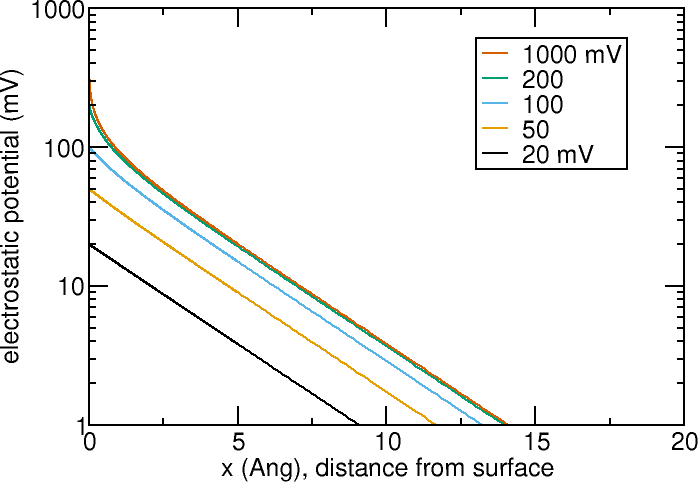
\includegraphics[width=0.45\linewidth]{counterion_potential.png}
(b)
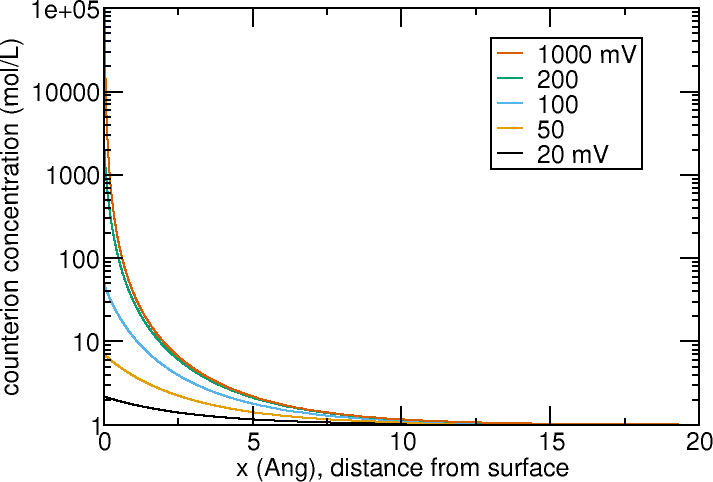
\includegraphics[width=0.45\linewidth]{counterion_logzero.png}
\caption{\label{fig_classical_PB}Solutions to the classical point
  charge Poisson-Boltzmann model of 1M NaCl electrolyte solution,
  shown as profiles along $x$, the perpendicular distance from an
  electrode surface (a) Electrostatic potential. (b) Counterion
  (\ce{Cl-}) concentration. }
\end{figure}

At still higher potentials the stability of simple log scaling with
respect to the coion must be considered. The coion, with same charge
as the electrostatic potential, is repelled from the electrode surface
with coion concentration trending towards zero at the electrode. At
sufficiently high potentials this generates values in the log-scaled
function that tend towards $-\infty$, which destabilises the numerical
solution. We therefore introduce a more complex log-scaling function,
\begin{equation}
Z_i(x) = \ln\left[c_i(x)/c_{i\infty}+1\right]/\ln 2 - 1
\label{log_zero}
\end{equation}
which keeps the scaled coion function constrained between -1 and 0
rather than $-\infty$ and 0. Since this scaling function addresses the
near-zero concentration of the coion, we call it ``log-zero'' scaling.

\section{Throttling algorithm}

Log-scaling of concentration functions makes a numerical solution to
the conventional Poisson-Boltzmann available at electrode potentials
up to 1.5V. Nevertheless \figref{fig_classical_PB}b demonstrates the
point charge catastrophe of the conventional model, with counterion
concentrations exceeding $10^{5}$ mol/L at the electrode
surface. Moreover, for general electrochemical applications it would
be desirable to be capable of obtaining solutions for electrode
potentials higher than 1.5V. To deal with the physical problem, we
introduce finite ion sizes with a steric force provided by the
Carnahan-Starling model, \eqnref{chem_pot_CS} (weak form
\eqnref{weak_CS}).  We apply ion volumes
$v_{\ce{Na}}=1.24 \text{\AA}^{3}$ per \ce{Na+} ion,
$v_{\ce{Cl}}=35.9 \text{\AA}^{3}$ per \ce{Cl-} ion (volumes taken from
quantum mechanical volumes of the ions' electron clouds
\cite{ParsonsNinham2009}).

The additional nonlinearity introduced by the Carnahan-Starling model,
where the chemical potential depends on the concentrations being
calculated, introduces a new challenge. The default nonlinear solver
in FEniCS assumes zero as an initial guess for the functions being
solved. But under the nonlinear conditions (with electrode potential
$>0.2$ V) where the Carnahan-Starling steric force is required, the
zero initial guess leads quickly to a diverging solution with infinite
residual. And yet a stable solution is accessible at lower values of
the boundary condition. We nudge the solver to a stable solution by
applying a throttling algorithm: reduce the boundary condition to a
small value for which a solution can be obtained, then incrementally
increase the boundary value back towards the target value, using the
previous found solution as an initial guess for the next
iteration. The approach is known to mathematicians as the homotopy
analysis method \cite{homotopy_analysis_Liao2012}, with our throttle
serving as a homotopy parameter applied to boundary conditions.
A flowchart for the algorithm is
shown in \figref{fig_throttling_algorithm}.

\begin{figure}
\centering
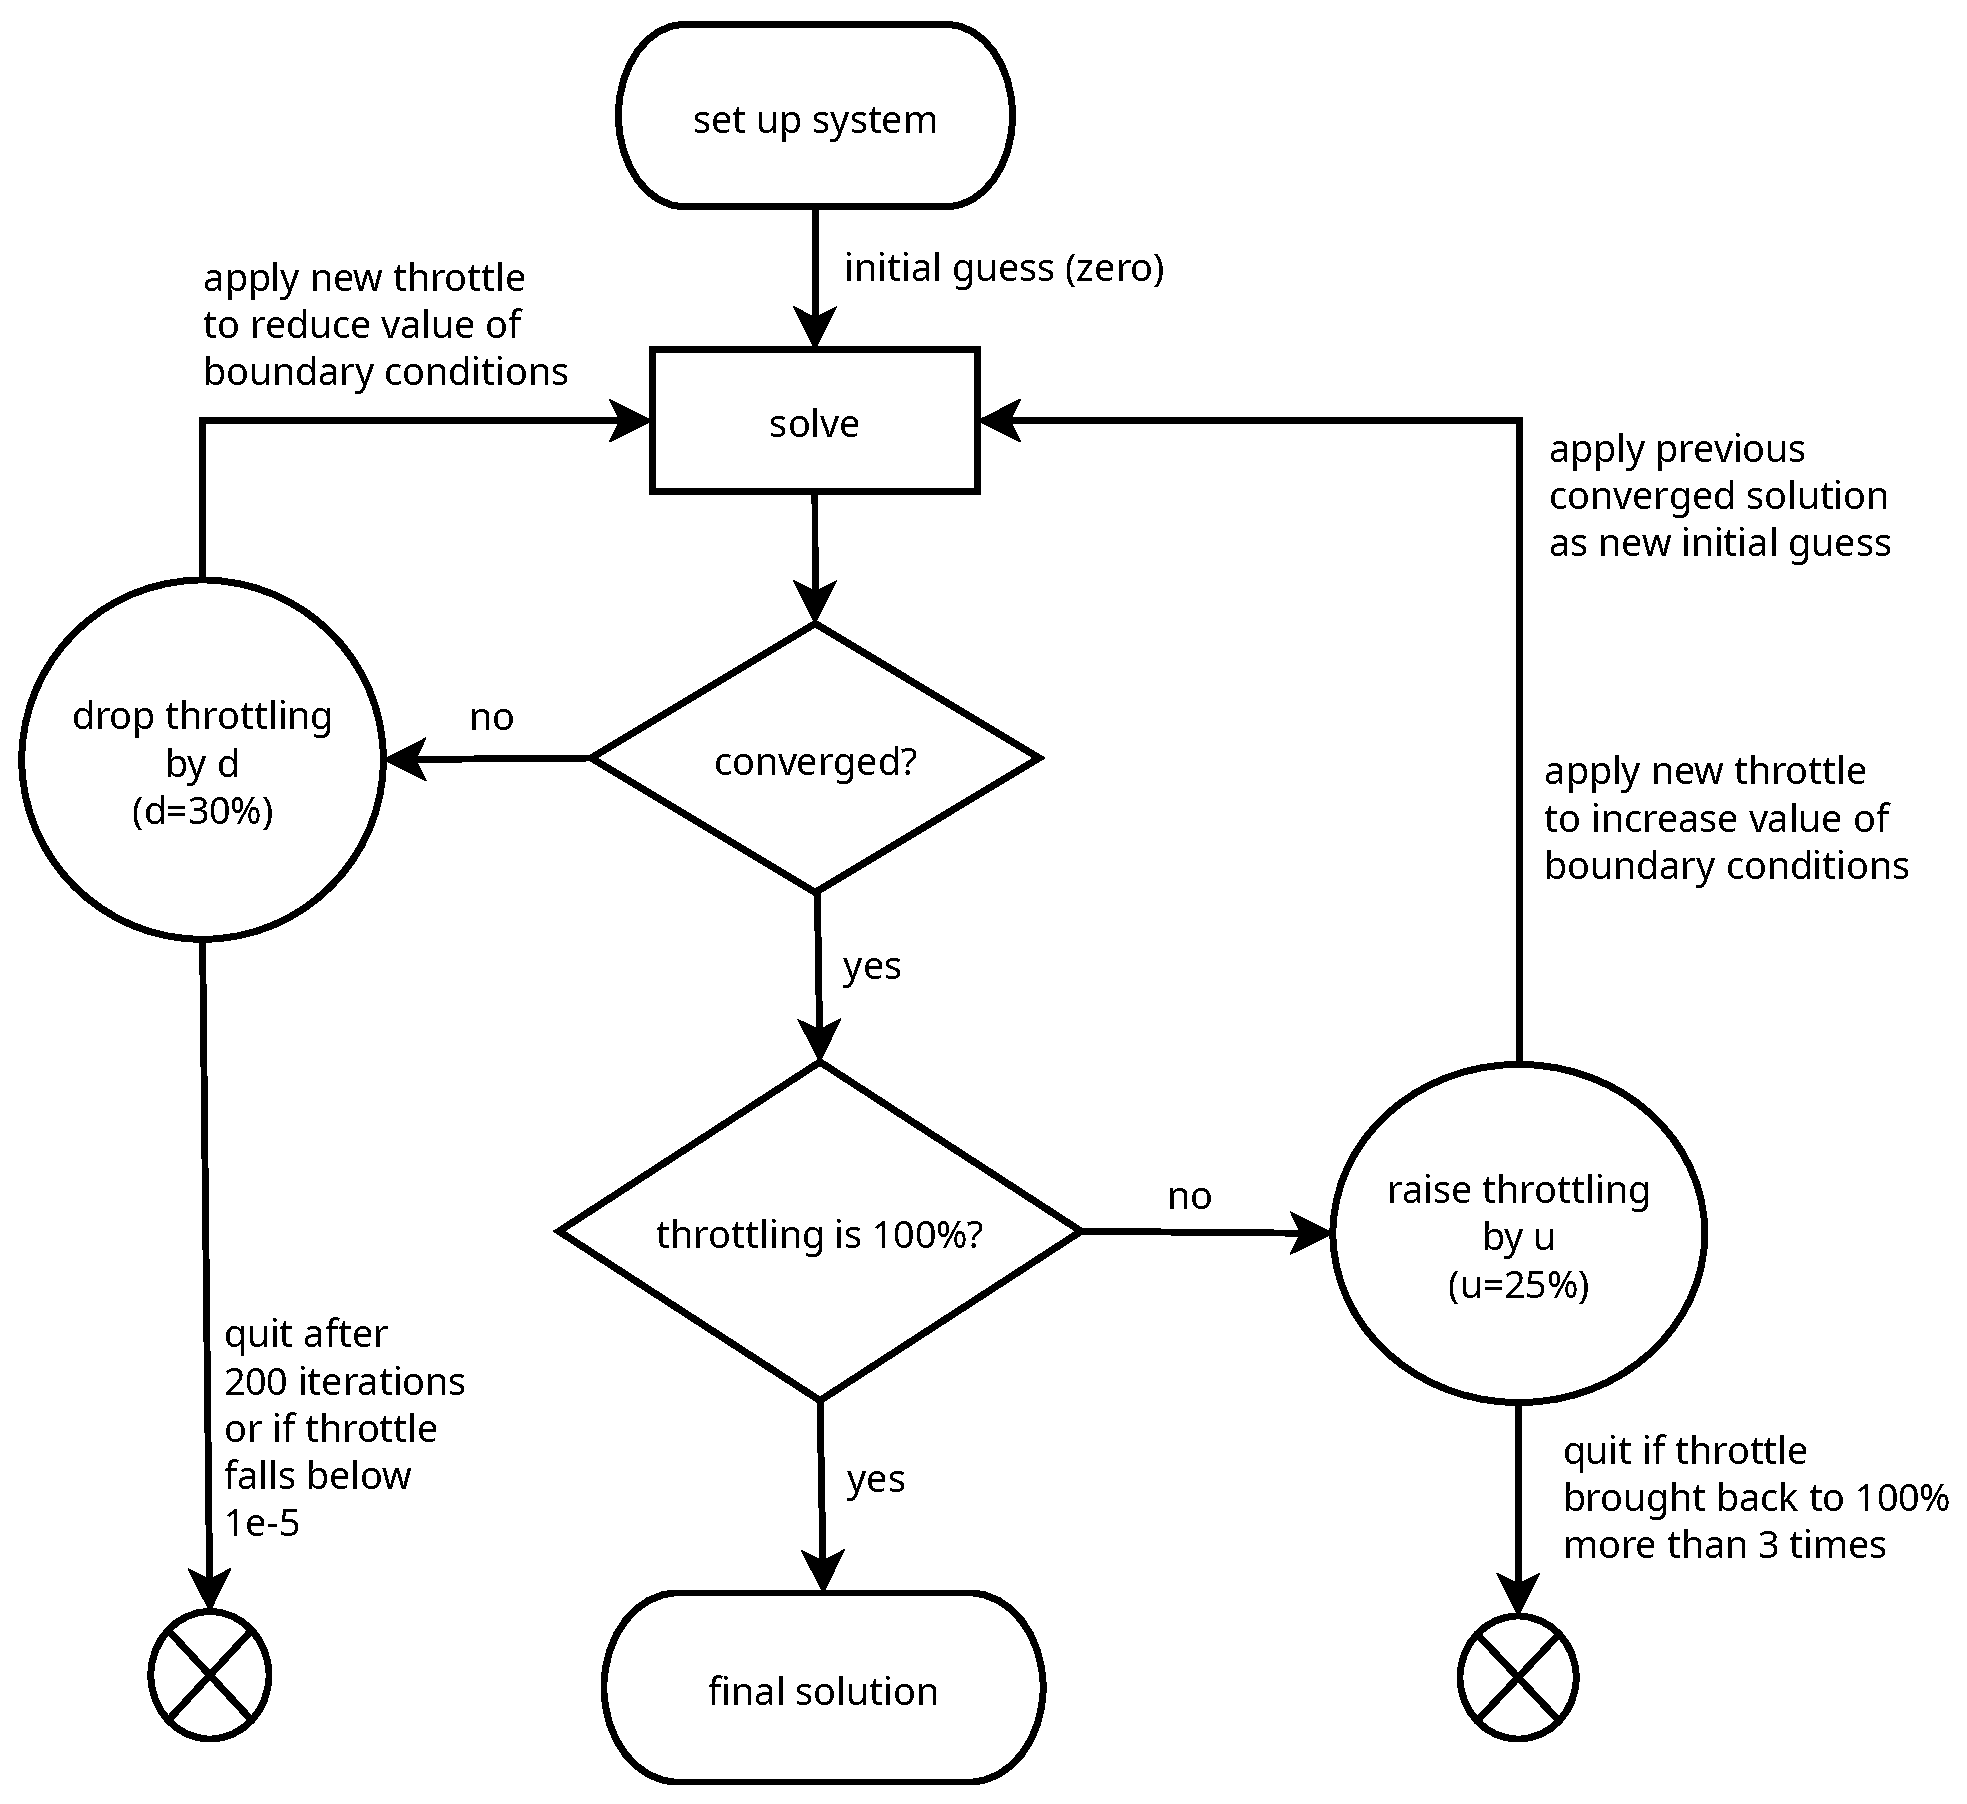
\includegraphics[width=0.8\linewidth]{throttling.eps}
\caption{\label{fig_throttling_algorithm}Flowchart for the throttling algorithm. }
\end{figure}

If the solver fails to converge, then reduce the throttle downwards to
a fraction $d$ of its previous value. The throttle is a multiplier
applied to the value of boundary conditions.  Once the boundary
condition is throttled enough to generate a converged solution, raise
the throttle upwards by an amount $u$, towards 100\% (set the throttle
to 100\% if the procedure would exceed it).  The values of $d$ and $u$
must find a balance between reaching 100\% throttle in as few
iterations as possible, while not collapsing back to non-converging
conditions when raising the throttle.  For potentials below 5V, we
find a drop level $d=75\%$ and a raise level $u=25\%$ with simple log
scaling of concentrations gives a reasonable balance between speed and
stability. If log-zero scaling is employed and the rise rate is
weakened to $u=10\%$, then electrode potentials of 20V can be
reached. With 5\% rising steps, 100V can be obtained. For a 1M
electrolyte, calculation at 240V would require such a small rise rate
that this algorithm becomes impractical.

If the throttling rates are not appropriately set, then the algorithm
may loop indefinitely between a converged solution at lower throttling
rate and non-convergence at a higher throttling rate. We therefore
halt after 200 throttle drops, or when the throttling rate drops below
$10^{-5}$, or when 100\% throttle is attempted more than 3 times.

The results of the throttling algorithm for an electrode charged to
10V, with Carnahan-Starling steric forces, is shown in
\figref{fig_results_throttling}. This solution was obtained with a
throttling rise rate of 10\% (0.1) and log-zero scaling of the
concentration functions
(\eqnref{log_zero}). \figref{fig_results_throttling} shows the onset
of a steric adsorption layer \cite{DagmawiParsons2022} with counterion
concentrations constrained below a concentration cap determined by the
ion size.

\begin{figure}
\centering
(a)
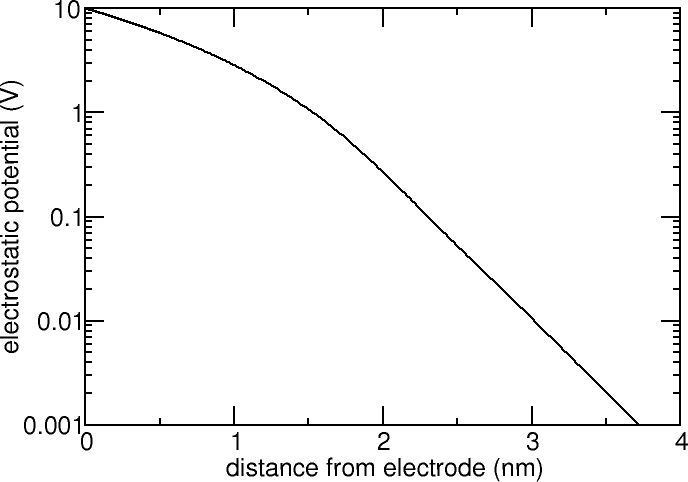
\includegraphics[width=0.4\linewidth]{steric_potential_10V.png}
(b)
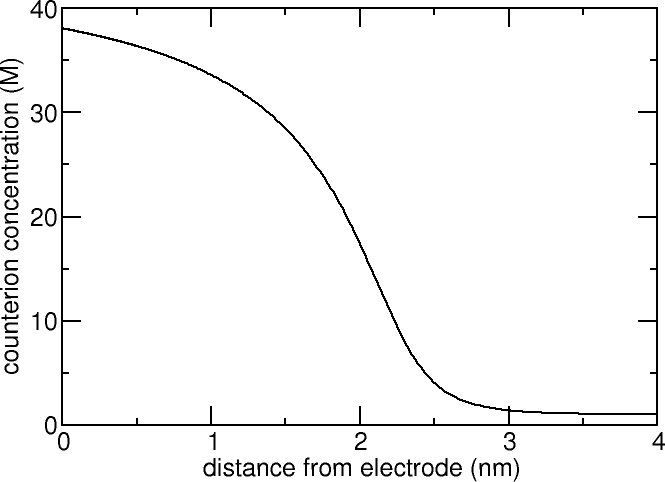
\includegraphics[width=0.4\linewidth]{steric_10V_counterion.png}
\caption{\label{fig_results_throttling}Solutions to the modified
  Poisson-Boltzmann model of a 1M NaCl electrolyte solution with
  Carnahan-Starling steric forces, shown as profiles along $x$, the
  perpendicular distance from a 5V electrode surface (a) Electrostatic
  potential. (b) Counterion (\ce{Cl-}) concentration. }
\end{figure}

\figref{fig_all_potential_high} presents algorithm conditions required
to obtains solutions (electrostatic potential profiles) up to
100V. Linear scaling (yellow region) is successful only for
$V<0.5$V. Log-scaling, \eqnref{log_scaling}, (purple region) with
throttling rise rate 25\% is successful up to 5V (purple
region). Log-zero scaling, \eqnref{log_zero}, with throttling rise
rate 10\% functions up to $V<20$V (blue region). Log-zero scaling with
5\% throttling rise rate can access up to $V<100$V (green region).

\begin{figure}
\centering
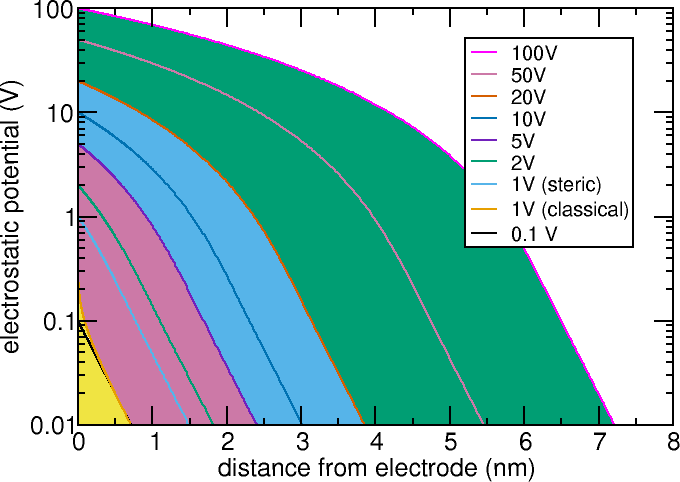
\includegraphics[width=0.9\linewidth]{counterion_potential_CS_bands.png}
\caption{\label{fig_all_potential_high} Algorithm conditions for
  electrostatic potential profiles with electrode potentials up to
  100V. Electrolyte is 1M NaCl. Linear scaling is functional for
  electrode potential $V<0.5$V (yellow region), log scaling (with
  steric forces) for $V<5$V with throttling rise rate 25\% (purple
  region), log-zero scaling with throttling rise rate 10\% for $V<20$V
  (blue region), and 5\% throttling rise rate for $V<100$V (green
  region).  }
\end{figure}

\section{Conclusion}

Modelling complex electrolyte solutions in electrochemical conditions
with electrode potentials 1V or greater requires both nontrivial
physics and nontrivial numerical algorithms. With respect to the
physics, aside from redox chemistry and electrolysis (not considered
here), the finite sizes of ions must be taken into consideration. With
respect to numerical convergence, we have proposed two
features. Firstly, we propose log-zero function scaling that accounts
not only for the heightened concentrations of counterions near an
electrode, but also the near-zero concentrations of coions. Secondly,
we propose a throttling algorithm that reduces boundary conditions
down to the linear regime where a solution is easily obtained, then
progressively propagating that solution by releasing the throttle
until the target boundary condition is obtained. The combination of
log-zero scaling and throttling enables calculations of electrolyte
solutions with electrode potentials up to 100V to be obtained. We
illustrated the throttling algorithm using Dirichlet boundary
conditions (electrode potentials), but the same principle applies
equally to Neumann or more complex boundary conditions.

\begin{acknowledgement}
  We acknowledge the award of CINECA support under the ISCRA
  initiative, for the availability of high-performance computing
  resources and support.
\end{acknowledgement}

\bibliographystyle{spbasic}
% Write the full path of your bibfile relative to book.tex
\bibliography{chapters/chp1/bibliography.bib}


 
% Write the full path to the location of the graphics relative to book.tex
\graphicspath{{chapters/chp1/graphics/}}

\title{Function scaling and throttling for convergence control in highly nonlinear Poisson-Boltzmann electrolyte models.}
\titlerunning{Function Scaling and Convergence Throttling}

\author{D.~F.~Parsons, M.~Farci,  A.~Grigoras, Dagmawi Tadesse}
\authorrunning{Parsons et al.}

\institute{D.~F.~Parsons \email{drew.parsons@unica.it}
  \and M.~Farci \and A.~Grigoras
  \at University of Cagliari,
Department of Chemical and Geological Sciences \& CSGI,
Cittadella Universitaria, S.S. 554 bivio Sestu,
09042 Monserrato (CA), Italy
\and Dagmawi Tadesse
\at Murdoch University,
Discipline of Physics, Chemistry and Mathematics, 90 South St, Murdoch 6150, West Australia
}

\maketitle

\abstract{ The nonlinear Poisson-Boltzmann model of electrolyte
  solutions combines the Poisson equation for electrostatic potentials
  with a Boltzmann equilibrium of mobile ion concentrations. The
  Boltzmann equation $c(x) = c_0 \exp[-q\psi(x)/kT]$ is highly
  nonlinear once the electrostatic potential exceeds several thermal
  energy ($kT$) units (i.e.\ when $\psi>0.1$ V). This introduces two
  related numerical challenges. Firstly, suitable convergence criteria
  for the concentration functions becomes variable, depending on the
  boundary potential. Secondly a controlled initial guess must be
  provided must be provided to avoid the FEM calculation diverging to
  NaN. We resolve the first by logarithmic scaling of the
  concentration function, as suggested by the exponential nature of
  the Boltzmann equation.  However a nontrivial complex logarithmic
  form is required in order to allow for the near-zero concentrations
  of coions, which would trigger numerical divergence in a trivial
  $\ln[c(x)]$ scaled function. The second challenge is resolved by
  iteratively with a throttling algorithm that suppresses large
  boundary conditions down to the linear regime, which is then applied
  as an initial guess for the nonlinear regime. Our implementation
  allows for other nonelectrostatic molecular interactions important
  for modelling real chemical and electrochemical systems, in
  particular steric forces due to finite ions sizes, enabling
  computation of concentrated electrolytes with electrode potentials
  as high as 100V.  }

\section*{Introduction}

Continuum theory (mean field theory) has been an effective tool for
studying the behaviour of systems in electrolyte solutions. The
Poisson-Boltzmann (PB) model \cite{Wu2022} enables evaluation of ion
adsorption layers at surfaces together with the electric field that
surface charge and adsorbed ions generate. Its nonequilibrium
counterpart, the Poisson-Nernst-Planck model
\cite{LopezGarciaHornoGrosse2018} (also called drift-diffusion)
likewise enables simulation of systems under conditions of moving
current. The PB model underpins theory of colloidal stability,
enabling modelling of nanoparticle aggregation and surface forces. The
same theory can in principle be applied to model electrochemical
systems, including energy storage devices, batteries or
supercapacitors. But there is a crucial difference in the two classes
of application, which has a significant impact on the numerical
stability of the model.  The surface potentials (or zeta potentials)
of typical colloidal systems such as protein molecules or metal oxide
particles tends to be found in the range 5--50 mV, which is 0.2--2
$kT$ in thermal energy units (based on a thermal potential at $T=298$
K defined by $e\psi_{T} = kT$ (where $e$ is the elementary charge, $k$
is Boltzmann's constant, $T$ is temperature). Electrolytic energy
storage systems, by contrast, typically operate with electrode
potentials of the order of 1--5 V, that is 1000--5000 mV, or 40--200
$kT$.  The nonlinearity of the Poisson-Boltzmann model is highly
sensitive to energies exceeding one $kT$ unit, requiring particular
algorithms to enable numerical nonlinear convergence.  Our goal is to
set up the calculation to solve successfully over a broad range of
electrode potentials without requiring manual readjustment of
convergence parameters.  We identify two main steps, implemented via
finite element methods (using FEniCSx\cite{baratta2023dolfinx}): log-scaling of
ion concentration functions, and throttling of boundary
conditions. For context we also present a summary of the physics and
weak formulation defining the Poisson-Boltzmann model, including
finite ion size effects. For simplicity we omit redox phenomenon
(electrolysis of water would occur in real systems at high electrode
potentials).

\section{Weak formulation of the Poisson-Boltzmann model}

The energy functional for an electrolyte solution, determined by
electrostatic potential $\psi(x)$ and ion concentration profiles
$c_i(x)$, may be composed from various fundamental energy
contributions as
\begin{equation}
    \Omega[\psi, c_i] = \Omega_{el} + \Omega_{en} +  \Omega_{ex}
\end{equation}
$\Omega_{el}$ describes the direct energy of the electrostatic field generated by the electric charge of ions and surfaces, \cite{Jackson}
\begin{equation}
  \Omega_{el}  =\frac{1}{2} \int_{V}D \cdot E dx
  = -\frac{1}{2} \int_{V}D \cdot E dx + \sum_i \int_V z_i e c_i(x) \psi(x) dx
  + \int_{S} \sigma(s) \psi(s) ds
\end{equation}
where $E$ is the electric field $E=-\nabla\psi$ and $D$ is the
electric displacement $D=\varepsilon_0
\varepsilon(x)E$. $\varepsilon_0$ is the permittivity of the vacuum,
and $\varepsilon(x)$ is the (spatially varying) relative
permittivity. $z_i$ is the valency of ion $i$.  $\sigma(s)$ is the
surface charge density on boundary $S$.

$\Omega_{en}$ describes the ideal entropic energy of ions, treated as ideal (noninteracting) particles \cite{GrayStiles2018,DagmawiParsons2024},
\begin{equation}
    \Omega_{en} = kT \sum_{i} \int_{V} \left[ c_i(x) \ln \left(\frac{c_i(x)}{c_{i\infty}} \right) - c_{i}(x) + c_{i\infty} \right] dx 
\end{equation}
where $c_{i\infty}$ is the bulk concentration of ions. As a point of
physics it is important to note that the use of a fixed bulk
concentration means the system is controlled by the chemical potential
of ions with a variable number of ions in the domain $V$ of interest.
That is, the thermodynamic potential is a grand potential, not a
(Helmholtz) free energy (hence we write the energy as $\Omega$ rather
than $F$). A free energy formulation (with fixed number of ions) would
require use of a thermal de Broglie wavelength instead of
$c_{i\infty}$ \cite{GrayStiles2018}.

$\Omega_{el} + \Omega_{en}$ alone construct the conventional
Poisson-Boltzmann model. The term $\Omega_{ex}$ represents extra
contributions to the total energy functional that describes other
relevant physics, such as pH-dependent charge regulation
\cite{ParsonsSalis2019}, specific ion interactions
\cite{ParsonsCarucciSalis2022}, or steric forces due to finite ion
size \cite{LopezGarciaHornoGrosse2018}. We consider the latter in this
work.

The Poisson-Boltzmann model describes the system in equilibrium,
obtained by minimising the total grand potential with variation
$\delta\Omega=0$ with respect to $\psi$ and $c_i$. Variation with
respect to $\psi$ (with test function $p$) leads to a weak formulation
for the Poisson equation,
\begin{equation}
    0 = -\int_{V} \varepsilon_{0}\varepsilon(x) (\nabla\psi,\nabla p) dx + \sum_{i}z_i e \int_{V} c_{i}(x) p dx + \int_{S} \sigma(s) p ds  
    \label{weak_Poisson}
\end{equation}
for all $p$ in the relevant finite element space.  After additional
integration by parts, this weak formulation leads to the strong
formulation of the electrostatic Poisson equation,
$\nabla\cdot D = \sum_i z_i e c_{i}(x)$. Variation $\delta\Omega$ with
respect to each ion concentration profile $c_i$ (in turn, with test
function $b_i$), assuming linear variations with
$\ln(1+b_i/c_i)=b_i/c_i$, leads to the weak formulation of Boltzmann's
equation,
\begin{equation}
    0 = \int_{V}z_i e \psi(x) b_i dx
    + kT \int_{V} b_i \ln\left(\frac{c_i(x)}{c_{i\infty}}\right)dx
    \label{weak_Boltzmann}
\end{equation}
for all $b_i$. The strong form of the classical Boltzmann equation can then obtained, $c_i(x)=c_{i\infty}\exp(-z_i e \psi(x)/kT)$. 

It might be noted that in the classical Poisson-Boltzmann model, the
ion concentrations $c_i$ are determined completely by the
electrostatic potential with the Boltzmann equation in closed form, so
only the Poisson equation needs solving directly. However, the
physical problem with the classical model is evident in electrochemical
systems with electrode potential 1 V. A one volt potential is
equivalent to a thermal energy of $40 kT)$, for which the conventional
Boltzmann factor for a counterion is
$\exp(40)\approx 2.3 \times 10^{17}$.  That is, the surface counterion
concentration of a 1M electrolyte would exceed $10^{17}$ mol/L, which
is obviously unphysical.  We return the model back to physical
relevance by adding an extra steric energy term $\Omega_{ex}$ with
corresponding excess chemical potential per ion $\mu_{i}^{ex}$, for
which the modified Boltzmann equation is
\begin{equation}
    c_i(x)=c_{i\infty}\exp\left[(-(z_i e \psi(x) + \mu_i^{ex}(x)-\mu_{i\infty}^{ex})/kT\right]
    \label{general_Boltzmann}
\end{equation}
$\mu_{i\infty}$ refers to the (fixed) excess chemical potential of the ion in bulk solution.
The steric model we employ is the Carnahan-Starling model \cite{CarnahanStarling1969} with grand potential
\begin{equation}
    \Omega_{ex} = \sum_{i} \int_{V} c_{i}(x) \left[ kT
    \frac{4\phi - 3\phi^2}{(1-\phi)^2}
    -  \mu_{\infty}
    \right]dx
\end{equation}
and weak formulation
\begin{equation}
    0 = \int_{V} (\mu_i^{ex}-\mu_{i\infty}^{ex}) b_i
    \label{weak_CS}
\end{equation}
for all $b_i$, which adds to \eqnref{weak_Boltzmann}, the weak
formulation for the Boltzmann equation, together generating the strong
formulation of \eqnref{general_Boltzmann}, the modified Boltzmann
equation.  Here we have introduced from the excess chemical potential
per ion for the Carnahan-Starling model,
\begin{equation}
    \mu_{i}^{ex} = kT \frac{\phi(8-9\phi+3\phi^2)}{(1-\phi)^3}
    \label{chem_pot_CS}
\end{equation}
Crucially, $\phi$ is the \emph{total} ion volume fraction defined by
$\phi=\sum_i c_i v_i$ where $v_i$ is the intrinsic molar volume per
ion $i$. Hence the CS excess chemical potential is defined identically
for all ions. To derive the weak formulation in \eqnref{weak_CS}, we
applied an homogenised component approximation that assigns common
volumes when introducing the test function $b_i$ (which is the
variation $\delta c_i$), such that $\delta\phi=v_j \delta c_i$ rather
than $v_i \delta c_i$. This approximation is required since the CS
model was formulated for single component systems. The more complex
multicomponent BMCSL model would enable ion specific chemical
potentials \cite{MansooriCarnahanStarlingLeland1971}, removing the
need for this approximation.  $\phi_{\infty}$, $\mu_{i\infty}^{ex}$
are the bulk total volume fraction and excess chemical potential
defined by bulk concentrations $c_{i\infty}$. With this term, the
Boltzmann equation is transcendental in $c_i$, precluding a closed
expression determining ion concentrations, which must therefore be
explicitly numerically solved alongside potential $\psi$. In this
paper we address strategies for managing the strong nonlinearity in
the system introduced by this term alongside large values of the
potential. Note that $c_i$ must also be solved explicitly in the case
of time-dependent nonequilibrium Poisson-Nernst-Planck systems where
ion concentrations are not in equilibrium and determined by a
continuity equation rather than a Boltzmann equation.

\section{Function scaling}
We constructed a finite element implementation of the weak
formulation(\eqnref{weak_Poisson} and \ref{weak_Boltzmann} (and
\eqnref{weak_CS}) in FEniCS-X \cite{baratta2023dolfinx}, using continuous
Lagrange elements with polynomial order 2.  The electrolyte solution
is taken as NaCl with bulk concentration 1 mol/L.  To illustrate
general issues of nonlinear convergence, we calculate the
electrostatic and ion concentration profiles of ion adsorbed at a
single flat electrode surface along the direction perpendicular to the
surface, with the electrode boundary at $x=0$.  The electrode
potential is controlled (Dirichlet boundary condition), and bulk
solution represented by a zero Neumann condition ("zero electric
field") at a distance of 30 Debye lengths (at $x=9.1$ nm, for the 1M
electrolyte). Nonlinear solutions are computed using FEniCS-X's
NonlinearProblem with a standard NewtonSolver. Convergence criterion
is set to FEniCS-X's default "incremental" method with absolute
tolerance $10^{-5}$.

We must consider scaling of the concentration functions $c_i(x)$. We
already noted that the counterion concentration becomes unphysically
large in the conventional Poisson-Boltzmann model due to nonlinear
exponentiation of the electrostatic potentials exceeding 0.1--0.2 V in
the Boltzmann equation. Trivial scaling may be introduced by solving
the concentration function scaled against the bulk concentration. But
with a convergence criterion of the nonlinear catastrophe is reached
numerically above 0.5 V. Already at 0.6 V, the conventional
calculation with simple scaling is unable to reduce the residual below
the required $10^{-5}$. While it would be possible to relax the
convergence tolerance to obtain a reasonable solution, our aim is to
obtain a robust general solver not requiring close manipulation of
convergence criteria. For instance, one application is modelling the
cyclic voltammetry curve of an electrode which require calculations
over a potential window as wide as $-5$ to 5 V.

The challenge arises due to the extreme magnitudes of the counterion
concentration at the electrode surface. The weak formulation for the
Boltzmann equation in \eqnref{weak_Boltzmann} suggests a solution:
solve for the concentration function in log-form,
\begin{equation}
C_{i}(x) = \ln[ c_{i}(x) / c_{i\infty}]
\label{log_scaling}
\end{equation}
rather than the concentration function $c_{i}(x)$ directly. Log
scaling extends the solvability of the conventional Poisson-Boltzmann
model up to electrode potentials as high as 1.5 V. Solutions for the
electrostatic potential and counterion concentration profile are shown
in \figref{fig_classical_PB}. Shown on a log scale, strong
nonlinearity in the PB system becomes apparent in the bend in the
electrostatic potential (\figref{fig_classical_PB}a) close to the
surface where $x<2$\AA for electrode potentials $> 0.2$ V.


\begin{figure}
\centering
(a)
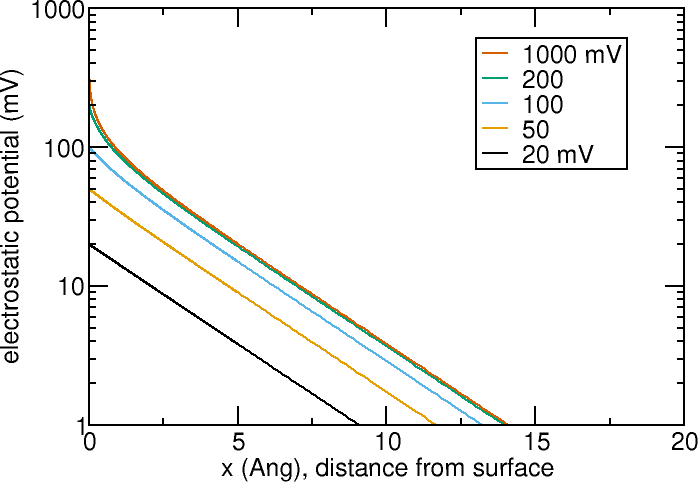
\includegraphics[width=0.45\linewidth]{counterion_potential.png}
(b)
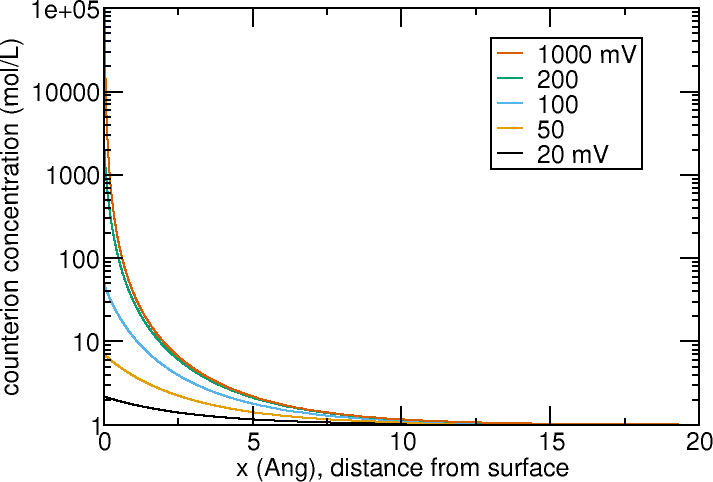
\includegraphics[width=0.45\linewidth]{counterion_logzero.png}
\caption{\label{fig_classical_PB}Solutions to the classical point
  charge Poisson-Boltzmann model of 1M NaCl electrolyte solution,
  shown as profiles along $x$, the perpendicular distance from an
  electrode surface (a) Electrostatic potential. (b) Counterion
  (\ce{Cl-}) concentration. }
\end{figure}

At still higher potentials the stability of simple log scaling with
respect to the coion must be considered. The coion, with same charge
as the electrostatic potential, is repelled from the electrode surface
with coion concentration trending towards zero at the electrode. At
sufficiently high potentials this generates values in the log-scaled
function that tend towards $-\infty$, which destabilises the numerical
solution. We therefore introduce a more complex log-scaling function,
\begin{equation}
Z_i(x) = \ln\left[c_i(x)/c_{i\infty}+1\right]/\ln 2 - 1
\label{log_zero}
\end{equation}
which keeps the scaled coion function constrained between -1 and 0
rather than $-\infty$ and 0. Since this scaling function addresses the
near-zero concentration of the coion, we call it ``log-zero'' scaling.

\section{Throttling algorithm}

Log-scaling of concentration functions makes a numerical solution to
the conventional Poisson-Boltzmann available at electrode potentials
up to 1.5V. Nevertheless \figref{fig_classical_PB}b demonstrates the
point charge catastrophe of the conventional model, with counterion
concentrations exceeding $10^{5}$ mol/L at the electrode
surface. Moreover, for general electrochemical applications it would
be desirable to be capable of obtaining solutions for electrode
potentials higher than 1.5V. To deal with the physical problem, we
introduce finite ion sizes with a steric force provided by the
Carnahan-Starling model, \eqnref{chem_pot_CS} (weak form
\eqnref{weak_CS}).  We apply ion volumes
$v_{\ce{Na}}=1.24 \text{\AA}^{3}$ per \ce{Na+} ion,
$v_{\ce{Cl}}=35.9 \text{\AA}^{3}$ per \ce{Cl-} ion (volumes taken from
quantum mechanical volumes of the ions' electron clouds
\cite{ParsonsNinham2009}).

The additional nonlinearity introduced by the Carnahan-Starling model,
where the chemical potential depends on the concentrations being
calculated, introduces a new challenge. The default nonlinear solver
in FEniCS assumes zero as an initial guess for the functions being
solved. But under the nonlinear conditions (with electrode potential
$>0.2$ V) where the Carnahan-Starling steric force is required, the
zero initial guess leads quickly to a diverging solution with infinite
residual. And yet a stable solution is accessible at lower values of
the boundary condition. We nudge the solver to a stable solution by
applying a throttling algorithm: reduce the boundary condition to a
small value for which a solution can be obtained, then incrementally
increase the boundary value back towards the target value, using the
previous found solution as an initial guess for the next
iteration. The approach is known to mathematicians as the homotopy
analysis method \cite{homotopy_analysis_Liao2012}, with our throttle
serving as a homotopy parameter applied to boundary conditions.
A flowchart for the algorithm is
shown in \figref{fig_throttling_algorithm}.

\begin{figure}
\centering
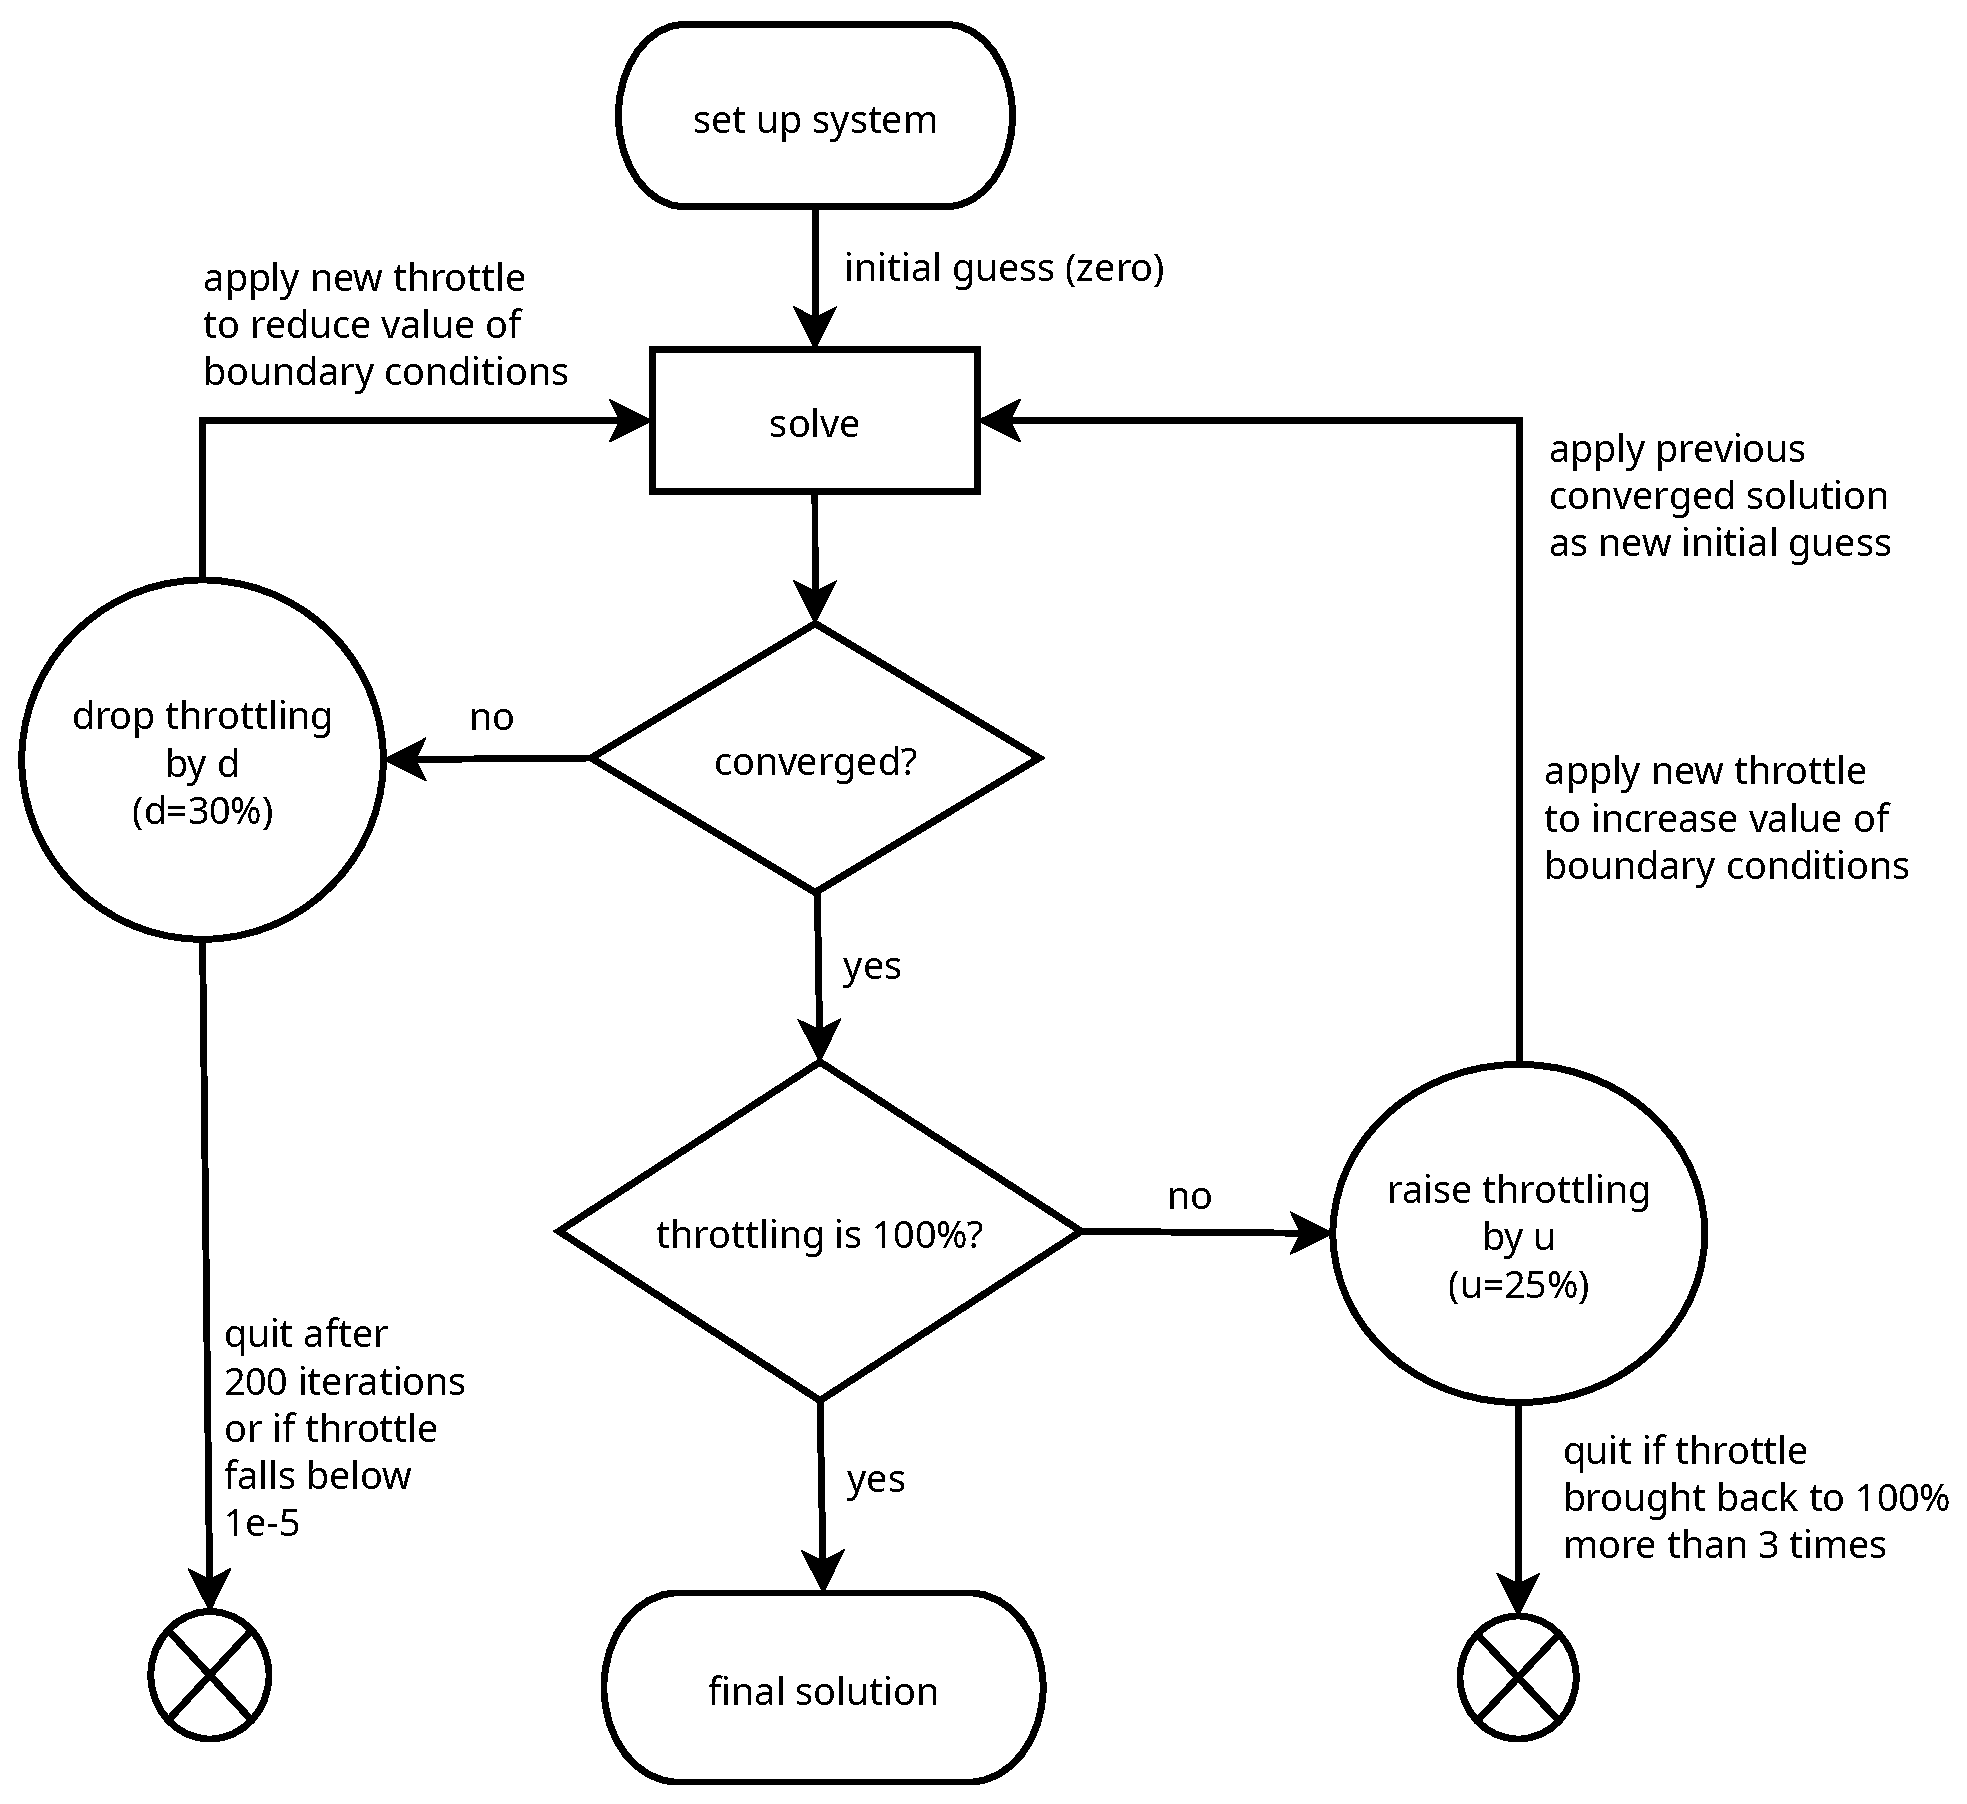
\includegraphics[width=0.8\linewidth]{throttling.eps}
\caption{\label{fig_throttling_algorithm}Flowchart for the throttling algorithm. }
\end{figure}

If the solver fails to converge, then reduce the throttle downwards to
a fraction $d$ of its previous value. The throttle is a multiplier
applied to the value of boundary conditions.  Once the boundary
condition is throttled enough to generate a converged solution, raise
the throttle upwards by an amount $u$, towards 100\% (set the throttle
to 100\% if the procedure would exceed it).  The values of $d$ and $u$
must find a balance between reaching 100\% throttle in as few
iterations as possible, while not collapsing back to non-converging
conditions when raising the throttle.  For potentials below 5V, we
find a drop level $d=75\%$ and a raise level $u=25\%$ with simple log
scaling of concentrations gives a reasonable balance between speed and
stability. If log-zero scaling is employed and the rise rate is
weakened to $u=10\%$, then electrode potentials of 20V can be
reached. With 5\% rising steps, 100V can be obtained. For a 1M
electrolyte, calculation at 240V would require such a small rise rate
that this algorithm becomes impractical.

If the throttling rates are not appropriately set, then the algorithm
may loop indefinitely between a converged solution at lower throttling
rate and non-convergence at a higher throttling rate. We therefore
halt after 200 throttle drops, or when the throttling rate drops below
$10^{-5}$, or when 100\% throttle is attempted more than 3 times.

The results of the throttling algorithm for an electrode charged to
10V, with Carnahan-Starling steric forces, is shown in
\figref{fig_results_throttling}. This solution was obtained with a
throttling rise rate of 10\% (0.1) and log-zero scaling of the
concentration functions
(\eqnref{log_zero}). \figref{fig_results_throttling} shows the onset
of a steric adsorption layer \cite{DagmawiParsons2022} with counterion
concentrations constrained below a concentration cap determined by the
ion size.

\begin{figure}
\centering
(a)
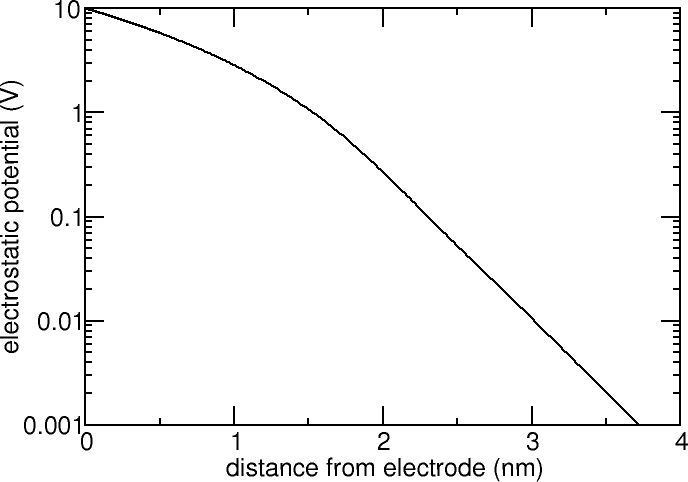
\includegraphics[width=0.4\linewidth]{steric_potential_10V.png}
(b)
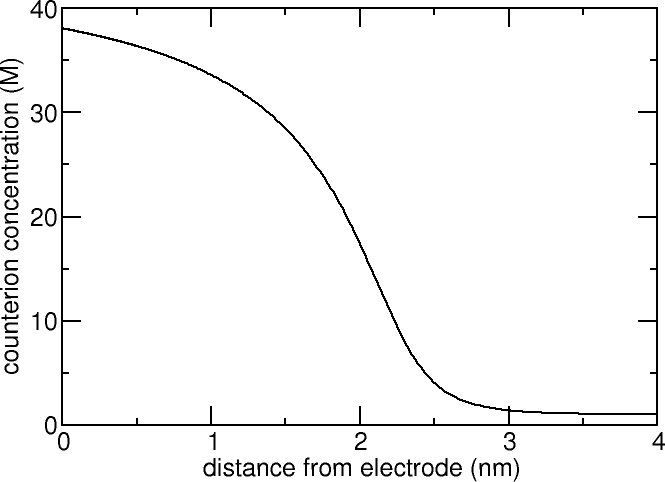
\includegraphics[width=0.4\linewidth]{steric_10V_counterion.png}
\caption{\label{fig_results_throttling}Solutions to the modified
  Poisson-Boltzmann model of a 1M NaCl electrolyte solution with
  Carnahan-Starling steric forces, shown as profiles along $x$, the
  perpendicular distance from a 5V electrode surface (a) Electrostatic
  potential. (b) Counterion (\ce{Cl-}) concentration. }
\end{figure}

\figref{fig_all_potential_high} presents algorithm conditions required
to obtains solutions (electrostatic potential profiles) up to
100V. Linear scaling (yellow region) is successful only for
$V<0.5$V. Log-scaling, \eqnref{log_scaling}, (purple region) with
throttling rise rate 25\% is successful up to 5V (purple
region). Log-zero scaling, \eqnref{log_zero}, with throttling rise
rate 10\% functions up to $V<20$V (blue region). Log-zero scaling with
5\% throttling rise rate can access up to $V<100$V (green region).

\begin{figure}
\centering
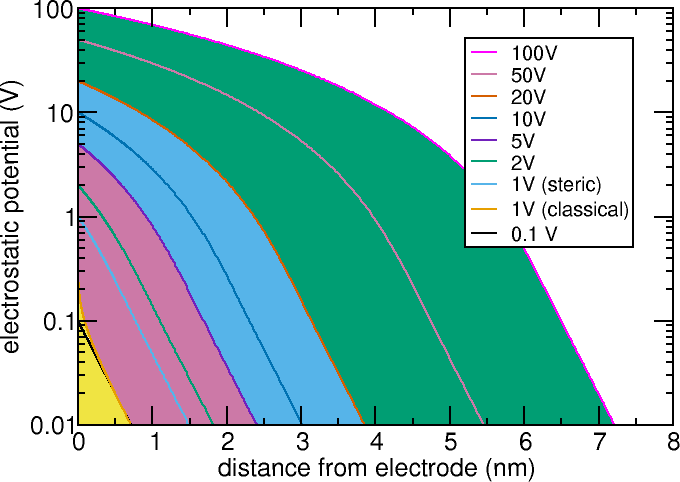
\includegraphics[width=0.9\linewidth]{counterion_potential_CS_bands.png}
\caption{\label{fig_all_potential_high} Algorithm conditions for
  electrostatic potential profiles with electrode potentials up to
  100V. Electrolyte is 1M NaCl. Linear scaling is functional for
  electrode potential $V<0.5$V (yellow region), log scaling (with
  steric forces) for $V<5$V with throttling rise rate 25\% (purple
  region), log-zero scaling with throttling rise rate 10\% for $V<20$V
  (blue region), and 5\% throttling rise rate for $V<100$V (green
  region).  }
\end{figure}

\section{Conclusion}

Modelling complex electrolyte solutions in electrochemical conditions
with electrode potentials 1V or greater requires both nontrivial
physics and nontrivial numerical algorithms. With respect to the
physics, aside from redox chemistry and electrolysis (not considered
here), the finite sizes of ions must be taken into consideration. With
respect to numerical convergence, we have proposed two
features. Firstly, we propose log-zero function scaling that accounts
not only for the heightened concentrations of counterions near an
electrode, but also the near-zero concentrations of coions. Secondly,
we propose a throttling algorithm that reduces boundary conditions
down to the linear regime where a solution is easily obtained, then
progressively propagating that solution by releasing the throttle
until the target boundary condition is obtained. The combination of
log-zero scaling and throttling enables calculations of electrolyte
solutions with electrode potentials up to 100V to be obtained. We
illustrated the throttling algorithm using Dirichlet boundary
conditions (electrode potentials), but the same principle applies
equally to Neumann or more complex boundary conditions.

\begin{acknowledgement}
  We acknowledge the award of CINECA support under the ISCRA
  initiative, for the availability of high-performance computing
  resources and support.
\end{acknowledgement}

\bibliographystyle{spbasic}
% Write the full path of your bibfile relative to book.tex
\bibliography{chapters/chp1/bibliography.bib}



% Write the full path to the location of the graphics relative to book.tex
\graphicspath{{chapters/chp1/graphics/}}

\title{Function scaling and throttling for convergence control in highly nonlinear Poisson-Boltzmann electrolyte models.}
\titlerunning{Function Scaling and Convergence Throttling}

\author{D.~F.~Parsons, M.~Farci,  A.~Grigoras, Dagmawi Tadesse}
\authorrunning{Parsons et al.}

\institute{D.~F.~Parsons \email{drew.parsons@unica.it}
  \and M.~Farci \and A.~Grigoras
  \at University of Cagliari,
Department of Chemical and Geological Sciences \& CSGI,
Cittadella Universitaria, S.S. 554 bivio Sestu,
09042 Monserrato (CA), Italy
\and Dagmawi Tadesse
\at Murdoch University,
Discipline of Physics, Chemistry and Mathematics, 90 South St, Murdoch 6150, West Australia
}

\maketitle

\abstract{ The nonlinear Poisson-Boltzmann model of electrolyte
  solutions combines the Poisson equation for electrostatic potentials
  with a Boltzmann equilibrium of mobile ion concentrations. The
  Boltzmann equation $c(x) = c_0 \exp[-q\psi(x)/kT]$ is highly
  nonlinear once the electrostatic potential exceeds several thermal
  energy ($kT$) units (i.e.\ when $\psi>0.1$ V). This introduces two
  related numerical challenges. Firstly, suitable convergence criteria
  for the concentration functions becomes variable, depending on the
  boundary potential. Secondly a controlled initial guess must be
  provided must be provided to avoid the FEM calculation diverging to
  NaN. We resolve the first by logarithmic scaling of the
  concentration function, as suggested by the exponential nature of
  the Boltzmann equation.  However a nontrivial complex logarithmic
  form is required in order to allow for the near-zero concentrations
  of coions, which would trigger numerical divergence in a trivial
  $\ln[c(x)]$ scaled function. The second challenge is resolved by
  iteratively with a throttling algorithm that suppresses large
  boundary conditions down to the linear regime, which is then applied
  as an initial guess for the nonlinear regime. Our implementation
  allows for other nonelectrostatic molecular interactions important
  for modelling real chemical and electrochemical systems, in
  particular steric forces due to finite ions sizes, enabling
  computation of concentrated electrolytes with electrode potentials
  as high as 100V.  }

\section*{Introduction}

Continuum theory (mean field theory) has been an effective tool for
studying the behaviour of systems in electrolyte solutions. The
Poisson-Boltzmann (PB) model \cite{Wu2022} enables evaluation of ion
adsorption layers at surfaces together with the electric field that
surface charge and adsorbed ions generate. Its nonequilibrium
counterpart, the Poisson-Nernst-Planck model
\cite{LopezGarciaHornoGrosse2018} (also called drift-diffusion)
likewise enables simulation of systems under conditions of moving
current. The PB model underpins theory of colloidal stability,
enabling modelling of nanoparticle aggregation and surface forces. The
same theory can in principle be applied to model electrochemical
systems, including energy storage devices, batteries or
supercapacitors. But there is a crucial difference in the two classes
of application, which has a significant impact on the numerical
stability of the model.  The surface potentials (or zeta potentials)
of typical colloidal systems such as protein molecules or metal oxide
particles tends to be found in the range 5--50 mV, which is 0.2--2
$kT$ in thermal energy units (based on a thermal potential at $T=298$
K defined by $e\psi_{T} = kT$ (where $e$ is the elementary charge, $k$
is Boltzmann's constant, $T$ is temperature). Electrolytic energy
storage systems, by contrast, typically operate with electrode
potentials of the order of 1--5 V, that is 1000--5000 mV, or 40--200
$kT$.  The nonlinearity of the Poisson-Boltzmann model is highly
sensitive to energies exceeding one $kT$ unit, requiring particular
algorithms to enable numerical nonlinear convergence.  Our goal is to
set up the calculation to solve successfully over a broad range of
electrode potentials without requiring manual readjustment of
convergence parameters.  We identify two main steps, implemented via
finite element methods (using FEniCSx\cite{baratta2023dolfinx}): log-scaling of
ion concentration functions, and throttling of boundary
conditions. For context we also present a summary of the physics and
weak formulation defining the Poisson-Boltzmann model, including
finite ion size effects. For simplicity we omit redox phenomenon
(electrolysis of water would occur in real systems at high electrode
potentials).

\section{Weak formulation of the Poisson-Boltzmann model}

The energy functional for an electrolyte solution, determined by
electrostatic potential $\psi(x)$ and ion concentration profiles
$c_i(x)$, may be composed from various fundamental energy
contributions as
\begin{equation}
    \Omega[\psi, c_i] = \Omega_{el} + \Omega_{en} +  \Omega_{ex}
\end{equation}
$\Omega_{el}$ describes the direct energy of the electrostatic field generated by the electric charge of ions and surfaces, \cite{Jackson}
\begin{equation}
  \Omega_{el}  =\frac{1}{2} \int_{V}D \cdot E dx
  = -\frac{1}{2} \int_{V}D \cdot E dx + \sum_i \int_V z_i e c_i(x) \psi(x) dx
  + \int_{S} \sigma(s) \psi(s) ds
\end{equation}
where $E$ is the electric field $E=-\nabla\psi$ and $D$ is the
electric displacement $D=\varepsilon_0
\varepsilon(x)E$. $\varepsilon_0$ is the permittivity of the vacuum,
and $\varepsilon(x)$ is the (spatially varying) relative
permittivity. $z_i$ is the valency of ion $i$.  $\sigma(s)$ is the
surface charge density on boundary $S$.

$\Omega_{en}$ describes the ideal entropic energy of ions, treated as ideal (noninteracting) particles \cite{GrayStiles2018,DagmawiParsons2024},
\begin{equation}
    \Omega_{en} = kT \sum_{i} \int_{V} \left[ c_i(x) \ln \left(\frac{c_i(x)}{c_{i\infty}} \right) - c_{i}(x) + c_{i\infty} \right] dx 
\end{equation}
where $c_{i\infty}$ is the bulk concentration of ions. As a point of
physics it is important to note that the use of a fixed bulk
concentration means the system is controlled by the chemical potential
of ions with a variable number of ions in the domain $V$ of interest.
That is, the thermodynamic potential is a grand potential, not a
(Helmholtz) free energy (hence we write the energy as $\Omega$ rather
than $F$). A free energy formulation (with fixed number of ions) would
require use of a thermal de Broglie wavelength instead of
$c_{i\infty}$ \cite{GrayStiles2018}.

$\Omega_{el} + \Omega_{en}$ alone construct the conventional
Poisson-Boltzmann model. The term $\Omega_{ex}$ represents extra
contributions to the total energy functional that describes other
relevant physics, such as pH-dependent charge regulation
\cite{ParsonsSalis2019}, specific ion interactions
\cite{ParsonsCarucciSalis2022}, or steric forces due to finite ion
size \cite{LopezGarciaHornoGrosse2018}. We consider the latter in this
work.

The Poisson-Boltzmann model describes the system in equilibrium,
obtained by minimising the total grand potential with variation
$\delta\Omega=0$ with respect to $\psi$ and $c_i$. Variation with
respect to $\psi$ (with test function $p$) leads to a weak formulation
for the Poisson equation,
\begin{equation}
    0 = -\int_{V} \varepsilon_{0}\varepsilon(x) (\nabla\psi,\nabla p) dx + \sum_{i}z_i e \int_{V} c_{i}(x) p dx + \int_{S} \sigma(s) p ds  
    \label{weak_Poisson}
\end{equation}
for all $p$ in the relevant finite element space.  After additional
integration by parts, this weak formulation leads to the strong
formulation of the electrostatic Poisson equation,
$\nabla\cdot D = \sum_i z_i e c_{i}(x)$. Variation $\delta\Omega$ with
respect to each ion concentration profile $c_i$ (in turn, with test
function $b_i$), assuming linear variations with
$\ln(1+b_i/c_i)=b_i/c_i$, leads to the weak formulation of Boltzmann's
equation,
\begin{equation}
    0 = \int_{V}z_i e \psi(x) b_i dx
    + kT \int_{V} b_i \ln\left(\frac{c_i(x)}{c_{i\infty}}\right)dx
    \label{weak_Boltzmann}
\end{equation}
for all $b_i$. The strong form of the classical Boltzmann equation can then obtained, $c_i(x)=c_{i\infty}\exp(-z_i e \psi(x)/kT)$. 

It might be noted that in the classical Poisson-Boltzmann model, the
ion concentrations $c_i$ are determined completely by the
electrostatic potential with the Boltzmann equation in closed form, so
only the Poisson equation needs solving directly. However, the
physical problem with the classical model is evident in electrochemical
systems with electrode potential 1 V. A one volt potential is
equivalent to a thermal energy of $40 kT)$, for which the conventional
Boltzmann factor for a counterion is
$\exp(40)\approx 2.3 \times 10^{17}$.  That is, the surface counterion
concentration of a 1M electrolyte would exceed $10^{17}$ mol/L, which
is obviously unphysical.  We return the model back to physical
relevance by adding an extra steric energy term $\Omega_{ex}$ with
corresponding excess chemical potential per ion $\mu_{i}^{ex}$, for
which the modified Boltzmann equation is
\begin{equation}
    c_i(x)=c_{i\infty}\exp\left[(-(z_i e \psi(x) + \mu_i^{ex}(x)-\mu_{i\infty}^{ex})/kT\right]
    \label{general_Boltzmann}
\end{equation}
$\mu_{i\infty}$ refers to the (fixed) excess chemical potential of the ion in bulk solution.
The steric model we employ is the Carnahan-Starling model \cite{CarnahanStarling1969} with grand potential
\begin{equation}
    \Omega_{ex} = \sum_{i} \int_{V} c_{i}(x) \left[ kT
    \frac{4\phi - 3\phi^2}{(1-\phi)^2}
    -  \mu_{\infty}
    \right]dx
\end{equation}
and weak formulation
\begin{equation}
    0 = \int_{V} (\mu_i^{ex}-\mu_{i\infty}^{ex}) b_i
    \label{weak_CS}
\end{equation}
for all $b_i$, which adds to \eqnref{weak_Boltzmann}, the weak
formulation for the Boltzmann equation, together generating the strong
formulation of \eqnref{general_Boltzmann}, the modified Boltzmann
equation.  Here we have introduced from the excess chemical potential
per ion for the Carnahan-Starling model,
\begin{equation}
    \mu_{i}^{ex} = kT \frac{\phi(8-9\phi+3\phi^2)}{(1-\phi)^3}
    \label{chem_pot_CS}
\end{equation}
Crucially, $\phi$ is the \emph{total} ion volume fraction defined by
$\phi=\sum_i c_i v_i$ where $v_i$ is the intrinsic molar volume per
ion $i$. Hence the CS excess chemical potential is defined identically
for all ions. To derive the weak formulation in \eqnref{weak_CS}, we
applied an homogenised component approximation that assigns common
volumes when introducing the test function $b_i$ (which is the
variation $\delta c_i$), such that $\delta\phi=v_j \delta c_i$ rather
than $v_i \delta c_i$. This approximation is required since the CS
model was formulated for single component systems. The more complex
multicomponent BMCSL model would enable ion specific chemical
potentials \cite{MansooriCarnahanStarlingLeland1971}, removing the
need for this approximation.  $\phi_{\infty}$, $\mu_{i\infty}^{ex}$
are the bulk total volume fraction and excess chemical potential
defined by bulk concentrations $c_{i\infty}$. With this term, the
Boltzmann equation is transcendental in $c_i$, precluding a closed
expression determining ion concentrations, which must therefore be
explicitly numerically solved alongside potential $\psi$. In this
paper we address strategies for managing the strong nonlinearity in
the system introduced by this term alongside large values of the
potential. Note that $c_i$ must also be solved explicitly in the case
of time-dependent nonequilibrium Poisson-Nernst-Planck systems where
ion concentrations are not in equilibrium and determined by a
continuity equation rather than a Boltzmann equation.

\section{Function scaling}
We constructed a finite element implementation of the weak
formulation(\eqnref{weak_Poisson} and \ref{weak_Boltzmann} (and
\eqnref{weak_CS}) in FEniCS-X \cite{baratta2023dolfinx}, using continuous
Lagrange elements with polynomial order 2.  The electrolyte solution
is taken as NaCl with bulk concentration 1 mol/L.  To illustrate
general issues of nonlinear convergence, we calculate the
electrostatic and ion concentration profiles of ion adsorbed at a
single flat electrode surface along the direction perpendicular to the
surface, with the electrode boundary at $x=0$.  The electrode
potential is controlled (Dirichlet boundary condition), and bulk
solution represented by a zero Neumann condition ("zero electric
field") at a distance of 30 Debye lengths (at $x=9.1$ nm, for the 1M
electrolyte). Nonlinear solutions are computed using FEniCS-X's
NonlinearProblem with a standard NewtonSolver. Convergence criterion
is set to FEniCS-X's default "incremental" method with absolute
tolerance $10^{-5}$.

We must consider scaling of the concentration functions $c_i(x)$. We
already noted that the counterion concentration becomes unphysically
large in the conventional Poisson-Boltzmann model due to nonlinear
exponentiation of the electrostatic potentials exceeding 0.1--0.2 V in
the Boltzmann equation. Trivial scaling may be introduced by solving
the concentration function scaled against the bulk concentration. But
with a convergence criterion of the nonlinear catastrophe is reached
numerically above 0.5 V. Already at 0.6 V, the conventional
calculation with simple scaling is unable to reduce the residual below
the required $10^{-5}$. While it would be possible to relax the
convergence tolerance to obtain a reasonable solution, our aim is to
obtain a robust general solver not requiring close manipulation of
convergence criteria. For instance, one application is modelling the
cyclic voltammetry curve of an electrode which require calculations
over a potential window as wide as $-5$ to 5 V.

The challenge arises due to the extreme magnitudes of the counterion
concentration at the electrode surface. The weak formulation for the
Boltzmann equation in \eqnref{weak_Boltzmann} suggests a solution:
solve for the concentration function in log-form,
\begin{equation}
C_{i}(x) = \ln[ c_{i}(x) / c_{i\infty}]
\label{log_scaling}
\end{equation}
rather than the concentration function $c_{i}(x)$ directly. Log
scaling extends the solvability of the conventional Poisson-Boltzmann
model up to electrode potentials as high as 1.5 V. Solutions for the
electrostatic potential and counterion concentration profile are shown
in \figref{fig_classical_PB}. Shown on a log scale, strong
nonlinearity in the PB system becomes apparent in the bend in the
electrostatic potential (\figref{fig_classical_PB}a) close to the
surface where $x<2$\AA for electrode potentials $> 0.2$ V.


\begin{figure}
\centering
(a)
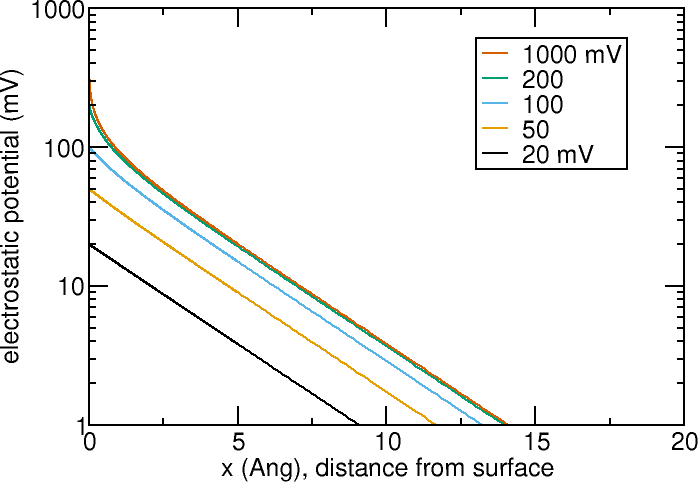
\includegraphics[width=0.45\linewidth]{counterion_potential.png}
(b)
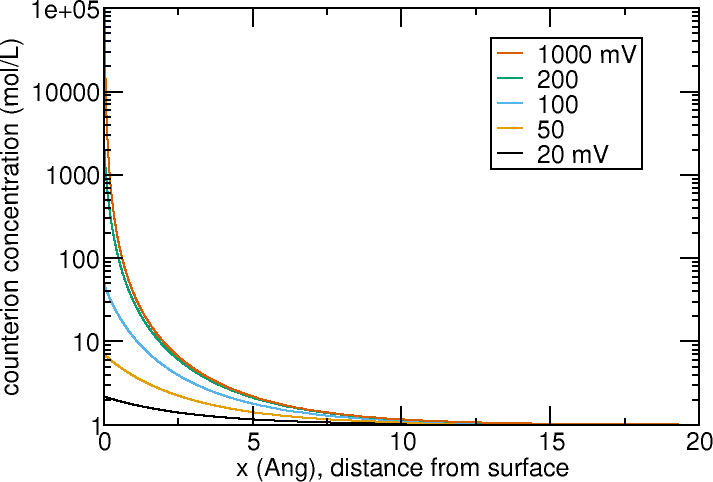
\includegraphics[width=0.45\linewidth]{counterion_logzero.png}
\caption{\label{fig_classical_PB}Solutions to the classical point
  charge Poisson-Boltzmann model of 1M NaCl electrolyte solution,
  shown as profiles along $x$, the perpendicular distance from an
  electrode surface (a) Electrostatic potential. (b) Counterion
  (\ce{Cl-}) concentration. }
\end{figure}

At still higher potentials the stability of simple log scaling with
respect to the coion must be considered. The coion, with same charge
as the electrostatic potential, is repelled from the electrode surface
with coion concentration trending towards zero at the electrode. At
sufficiently high potentials this generates values in the log-scaled
function that tend towards $-\infty$, which destabilises the numerical
solution. We therefore introduce a more complex log-scaling function,
\begin{equation}
Z_i(x) = \ln\left[c_i(x)/c_{i\infty}+1\right]/\ln 2 - 1
\label{log_zero}
\end{equation}
which keeps the scaled coion function constrained between -1 and 0
rather than $-\infty$ and 0. Since this scaling function addresses the
near-zero concentration of the coion, we call it ``log-zero'' scaling.

\section{Throttling algorithm}

Log-scaling of concentration functions makes a numerical solution to
the conventional Poisson-Boltzmann available at electrode potentials
up to 1.5V. Nevertheless \figref{fig_classical_PB}b demonstrates the
point charge catastrophe of the conventional model, with counterion
concentrations exceeding $10^{5}$ mol/L at the electrode
surface. Moreover, for general electrochemical applications it would
be desirable to be capable of obtaining solutions for electrode
potentials higher than 1.5V. To deal with the physical problem, we
introduce finite ion sizes with a steric force provided by the
Carnahan-Starling model, \eqnref{chem_pot_CS} (weak form
\eqnref{weak_CS}).  We apply ion volumes
$v_{\ce{Na}}=1.24 \text{\AA}^{3}$ per \ce{Na+} ion,
$v_{\ce{Cl}}=35.9 \text{\AA}^{3}$ per \ce{Cl-} ion (volumes taken from
quantum mechanical volumes of the ions' electron clouds
\cite{ParsonsNinham2009}).

The additional nonlinearity introduced by the Carnahan-Starling model,
where the chemical potential depends on the concentrations being
calculated, introduces a new challenge. The default nonlinear solver
in FEniCS assumes zero as an initial guess for the functions being
solved. But under the nonlinear conditions (with electrode potential
$>0.2$ V) where the Carnahan-Starling steric force is required, the
zero initial guess leads quickly to a diverging solution with infinite
residual. And yet a stable solution is accessible at lower values of
the boundary condition. We nudge the solver to a stable solution by
applying a throttling algorithm: reduce the boundary condition to a
small value for which a solution can be obtained, then incrementally
increase the boundary value back towards the target value, using the
previous found solution as an initial guess for the next
iteration. The approach is known to mathematicians as the homotopy
analysis method \cite{homotopy_analysis_Liao2012}, with our throttle
serving as a homotopy parameter applied to boundary conditions.
A flowchart for the algorithm is
shown in \figref{fig_throttling_algorithm}.

\begin{figure}
\centering
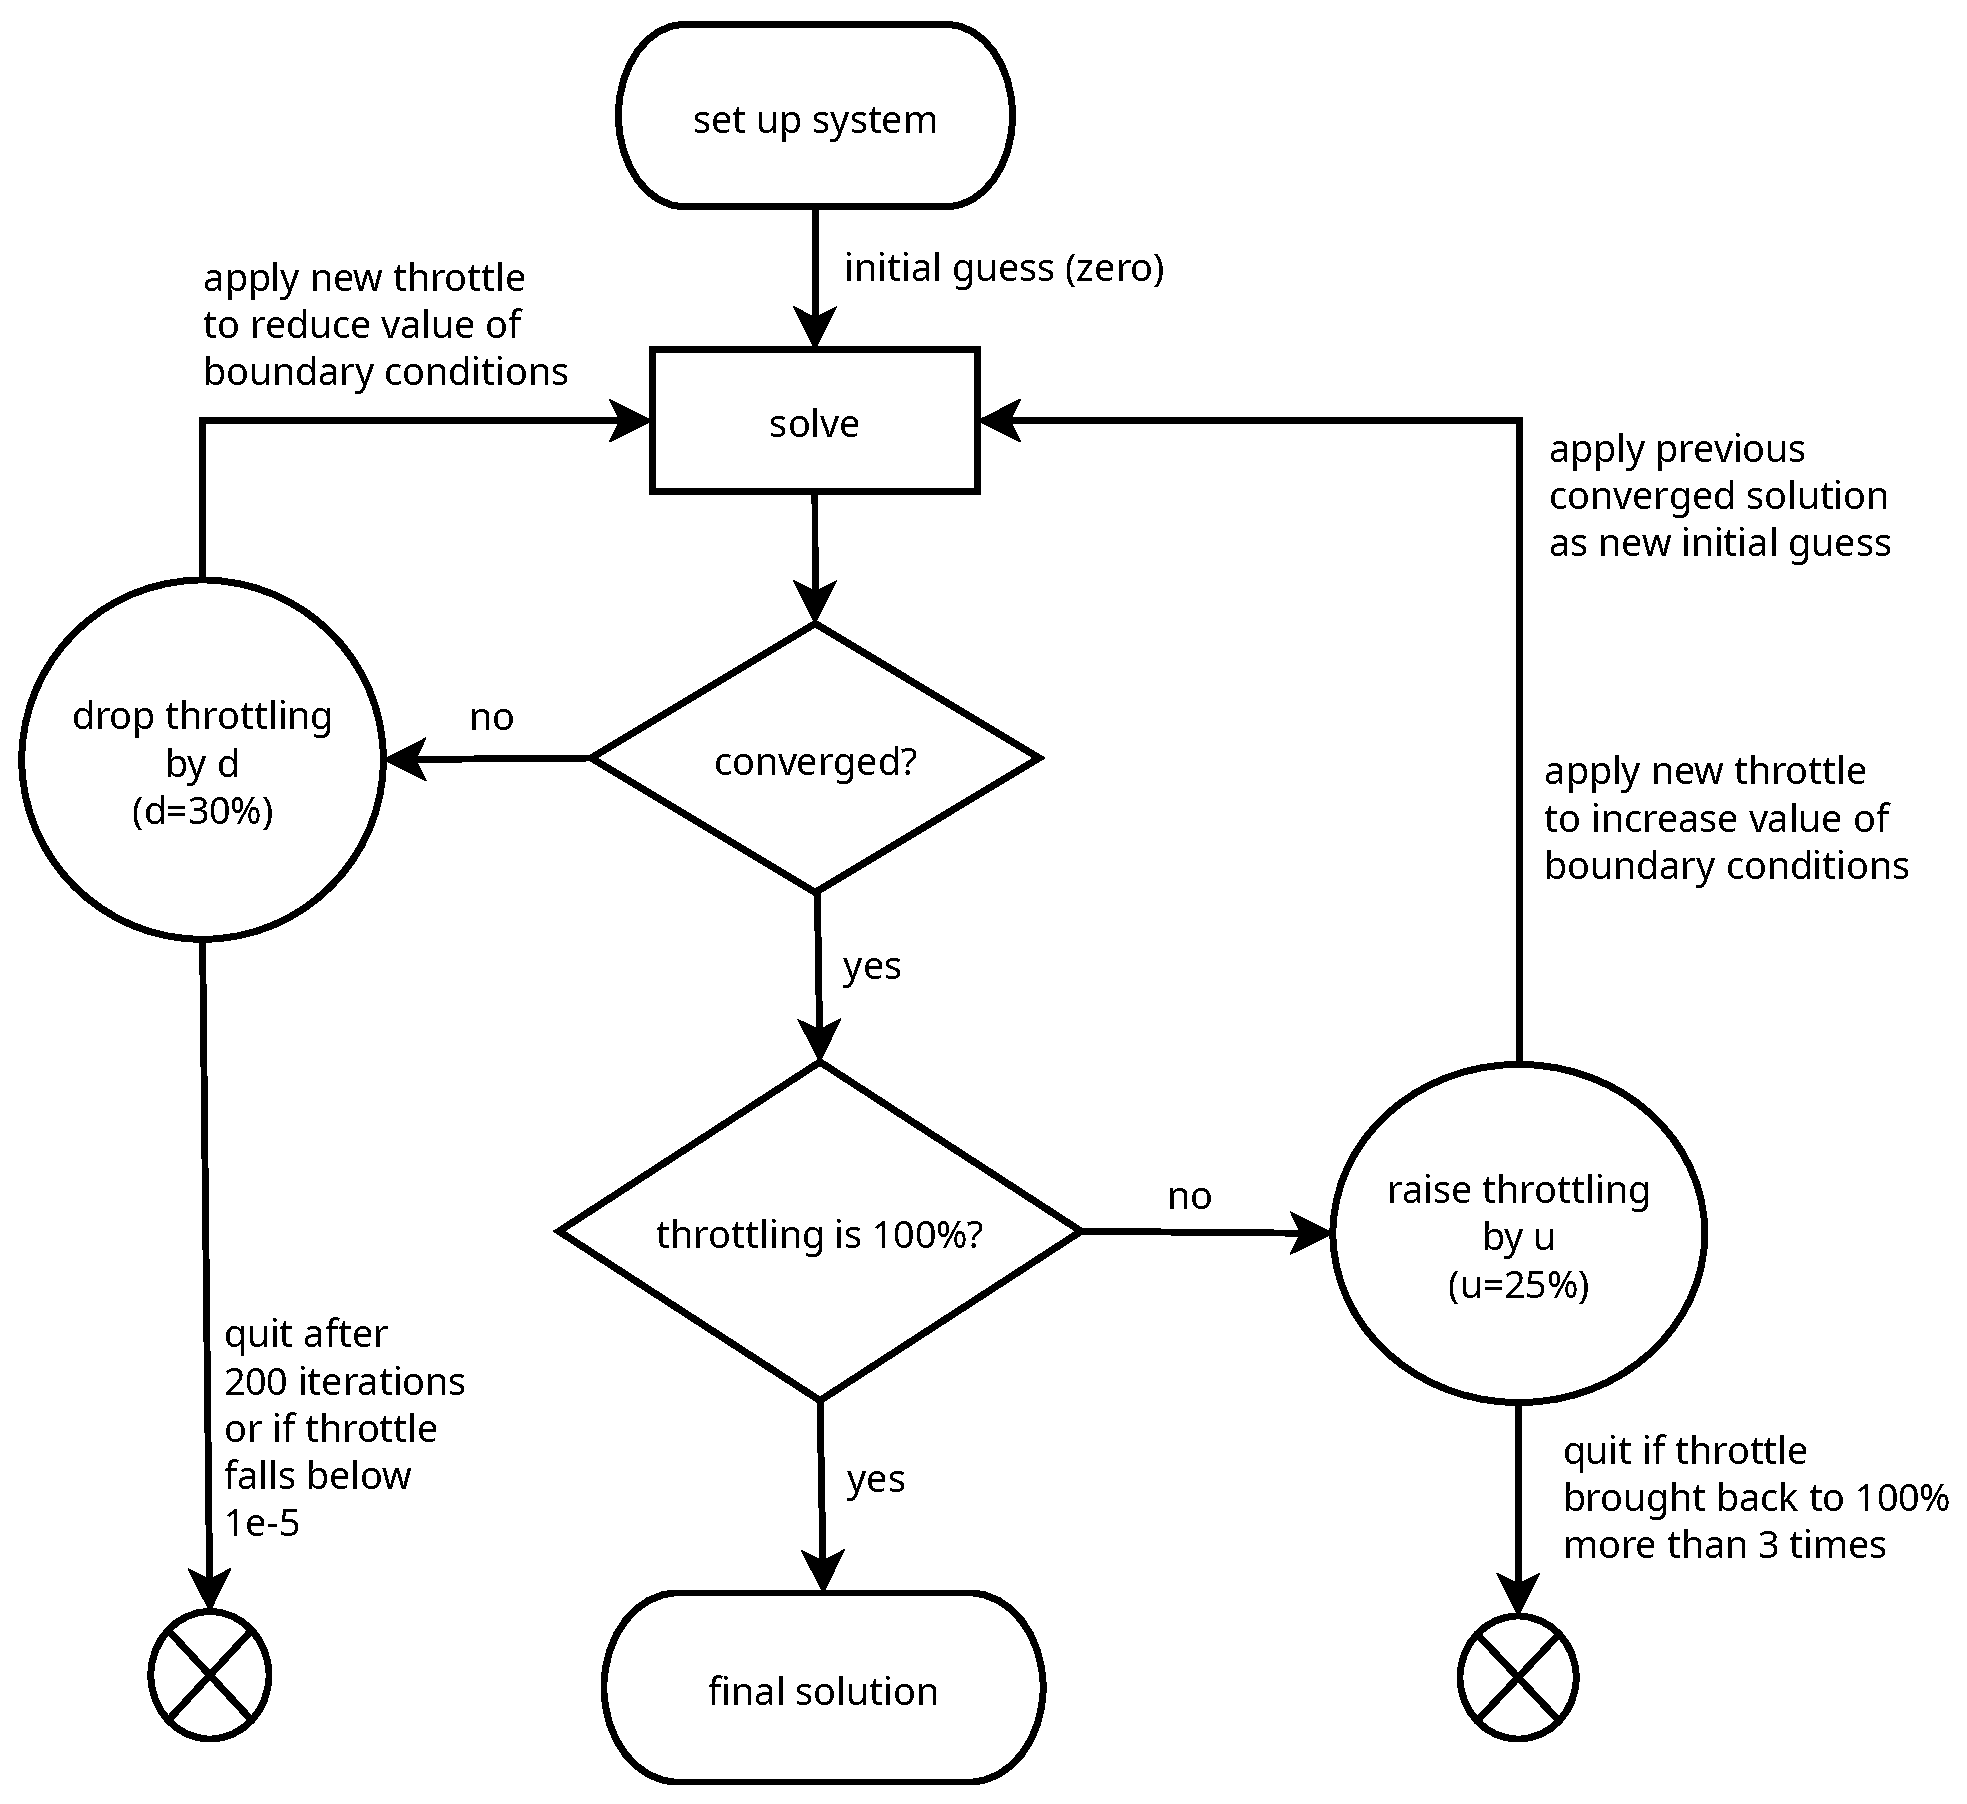
\includegraphics[width=0.8\linewidth]{throttling.eps}
\caption{\label{fig_throttling_algorithm}Flowchart for the throttling algorithm. }
\end{figure}

If the solver fails to converge, then reduce the throttle downwards to
a fraction $d$ of its previous value. The throttle is a multiplier
applied to the value of boundary conditions.  Once the boundary
condition is throttled enough to generate a converged solution, raise
the throttle upwards by an amount $u$, towards 100\% (set the throttle
to 100\% if the procedure would exceed it).  The values of $d$ and $u$
must find a balance between reaching 100\% throttle in as few
iterations as possible, while not collapsing back to non-converging
conditions when raising the throttle.  For potentials below 5V, we
find a drop level $d=75\%$ and a raise level $u=25\%$ with simple log
scaling of concentrations gives a reasonable balance between speed and
stability. If log-zero scaling is employed and the rise rate is
weakened to $u=10\%$, then electrode potentials of 20V can be
reached. With 5\% rising steps, 100V can be obtained. For a 1M
electrolyte, calculation at 240V would require such a small rise rate
that this algorithm becomes impractical.

If the throttling rates are not appropriately set, then the algorithm
may loop indefinitely between a converged solution at lower throttling
rate and non-convergence at a higher throttling rate. We therefore
halt after 200 throttle drops, or when the throttling rate drops below
$10^{-5}$, or when 100\% throttle is attempted more than 3 times.

The results of the throttling algorithm for an electrode charged to
10V, with Carnahan-Starling steric forces, is shown in
\figref{fig_results_throttling}. This solution was obtained with a
throttling rise rate of 10\% (0.1) and log-zero scaling of the
concentration functions
(\eqnref{log_zero}). \figref{fig_results_throttling} shows the onset
of a steric adsorption layer \cite{DagmawiParsons2022} with counterion
concentrations constrained below a concentration cap determined by the
ion size.

\begin{figure}
\centering
(a)
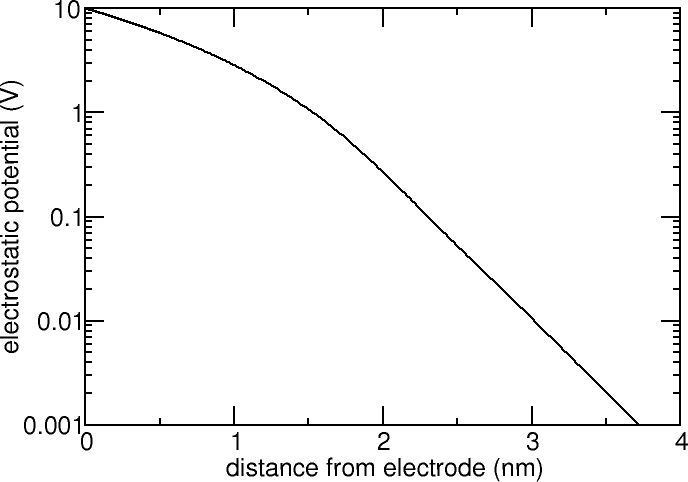
\includegraphics[width=0.4\linewidth]{steric_potential_10V.png}
(b)
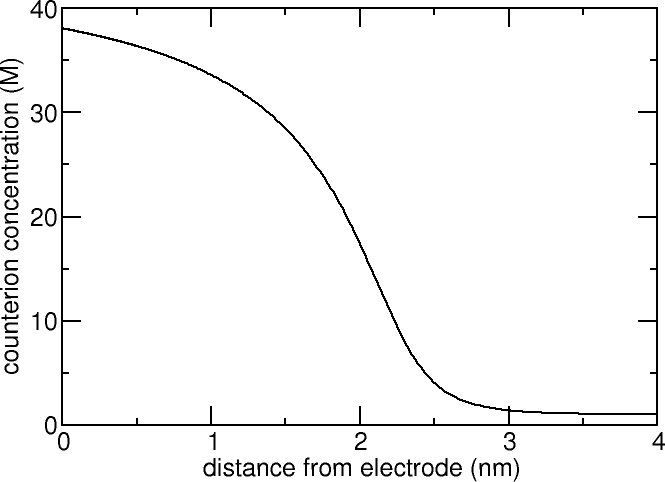
\includegraphics[width=0.4\linewidth]{steric_10V_counterion.png}
\caption{\label{fig_results_throttling}Solutions to the modified
  Poisson-Boltzmann model of a 1M NaCl electrolyte solution with
  Carnahan-Starling steric forces, shown as profiles along $x$, the
  perpendicular distance from a 5V electrode surface (a) Electrostatic
  potential. (b) Counterion (\ce{Cl-}) concentration. }
\end{figure}

\figref{fig_all_potential_high} presents algorithm conditions required
to obtains solutions (electrostatic potential profiles) up to
100V. Linear scaling (yellow region) is successful only for
$V<0.5$V. Log-scaling, \eqnref{log_scaling}, (purple region) with
throttling rise rate 25\% is successful up to 5V (purple
region). Log-zero scaling, \eqnref{log_zero}, with throttling rise
rate 10\% functions up to $V<20$V (blue region). Log-zero scaling with
5\% throttling rise rate can access up to $V<100$V (green region).

\begin{figure}
\centering
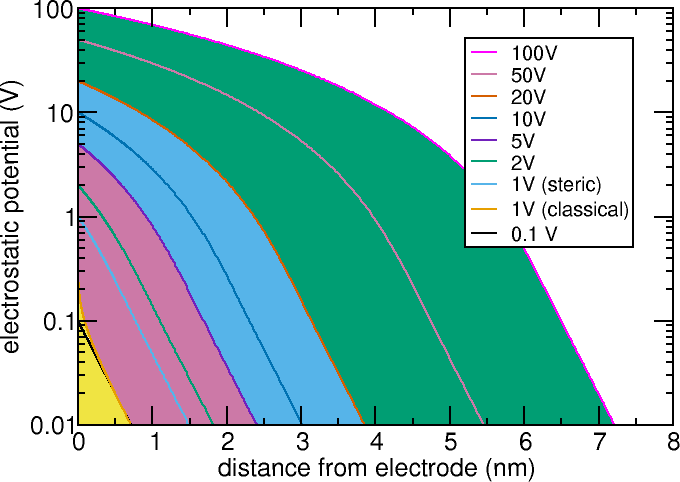
\includegraphics[width=0.9\linewidth]{counterion_potential_CS_bands.png}
\caption{\label{fig_all_potential_high} Algorithm conditions for
  electrostatic potential profiles with electrode potentials up to
  100V. Electrolyte is 1M NaCl. Linear scaling is functional for
  electrode potential $V<0.5$V (yellow region), log scaling (with
  steric forces) for $V<5$V with throttling rise rate 25\% (purple
  region), log-zero scaling with throttling rise rate 10\% for $V<20$V
  (blue region), and 5\% throttling rise rate for $V<100$V (green
  region).  }
\end{figure}

\section{Conclusion}

Modelling complex electrolyte solutions in electrochemical conditions
with electrode potentials 1V or greater requires both nontrivial
physics and nontrivial numerical algorithms. With respect to the
physics, aside from redox chemistry and electrolysis (not considered
here), the finite sizes of ions must be taken into consideration. With
respect to numerical convergence, we have proposed two
features. Firstly, we propose log-zero function scaling that accounts
not only for the heightened concentrations of counterions near an
electrode, but also the near-zero concentrations of coions. Secondly,
we propose a throttling algorithm that reduces boundary conditions
down to the linear regime where a solution is easily obtained, then
progressively propagating that solution by releasing the throttle
until the target boundary condition is obtained. The combination of
log-zero scaling and throttling enables calculations of electrolyte
solutions with electrode potentials up to 100V to be obtained. We
illustrated the throttling algorithm using Dirichlet boundary
conditions (electrode potentials), but the same principle applies
equally to Neumann or more complex boundary conditions.

\begin{acknowledgement}
  We acknowledge the award of CINECA support under the ISCRA
  initiative, for the availability of high-performance computing
  resources and support.
\end{acknowledgement}

\bibliographystyle{spbasic}
% Write the full path of your bibfile relative to book.tex
\bibliography{chapters/chp1/bibliography.bib}



% Write the full path to the location of the graphics relative to book.tex
\graphicspath{{chapters/chp1/graphics/}}

\title{Function scaling and throttling for convergence control in highly nonlinear Poisson-Boltzmann electrolyte models.}
\titlerunning{Function Scaling and Convergence Throttling}

\author{D.~F.~Parsons, M.~Farci,  A.~Grigoras, Dagmawi Tadesse}
\authorrunning{Parsons et al.}

\institute{D.~F.~Parsons \email{drew.parsons@unica.it}
  \and M.~Farci \and A.~Grigoras
  \at University of Cagliari,
Department of Chemical and Geological Sciences \& CSGI,
Cittadella Universitaria, S.S. 554 bivio Sestu,
09042 Monserrato (CA), Italy
\and Dagmawi Tadesse
\at Murdoch University,
Discipline of Physics, Chemistry and Mathematics, 90 South St, Murdoch 6150, West Australia
}

\maketitle

\abstract{ The nonlinear Poisson-Boltzmann model of electrolyte
  solutions combines the Poisson equation for electrostatic potentials
  with a Boltzmann equilibrium of mobile ion concentrations. The
  Boltzmann equation $c(x) = c_0 \exp[-q\psi(x)/kT]$ is highly
  nonlinear once the electrostatic potential exceeds several thermal
  energy ($kT$) units (i.e.\ when $\psi>0.1$ V). This introduces two
  related numerical challenges. Firstly, suitable convergence criteria
  for the concentration functions becomes variable, depending on the
  boundary potential. Secondly a controlled initial guess must be
  provided must be provided to avoid the FEM calculation diverging to
  NaN. We resolve the first by logarithmic scaling of the
  concentration function, as suggested by the exponential nature of
  the Boltzmann equation.  However a nontrivial complex logarithmic
  form is required in order to allow for the near-zero concentrations
  of coions, which would trigger numerical divergence in a trivial
  $\ln[c(x)]$ scaled function. The second challenge is resolved by
  iteratively with a throttling algorithm that suppresses large
  boundary conditions down to the linear regime, which is then applied
  as an initial guess for the nonlinear regime. Our implementation
  allows for other nonelectrostatic molecular interactions important
  for modelling real chemical and electrochemical systems, in
  particular steric forces due to finite ions sizes, enabling
  computation of concentrated electrolytes with electrode potentials
  as high as 100V.  }

\section*{Introduction}

Continuum theory (mean field theory) has been an effective tool for
studying the behaviour of systems in electrolyte solutions. The
Poisson-Boltzmann (PB) model \cite{Wu2022} enables evaluation of ion
adsorption layers at surfaces together with the electric field that
surface charge and adsorbed ions generate. Its nonequilibrium
counterpart, the Poisson-Nernst-Planck model
\cite{LopezGarciaHornoGrosse2018} (also called drift-diffusion)
likewise enables simulation of systems under conditions of moving
current. The PB model underpins theory of colloidal stability,
enabling modelling of nanoparticle aggregation and surface forces. The
same theory can in principle be applied to model electrochemical
systems, including energy storage devices, batteries or
supercapacitors. But there is a crucial difference in the two classes
of application, which has a significant impact on the numerical
stability of the model.  The surface potentials (or zeta potentials)
of typical colloidal systems such as protein molecules or metal oxide
particles tends to be found in the range 5--50 mV, which is 0.2--2
$kT$ in thermal energy units (based on a thermal potential at $T=298$
K defined by $e\psi_{T} = kT$ (where $e$ is the elementary charge, $k$
is Boltzmann's constant, $T$ is temperature). Electrolytic energy
storage systems, by contrast, typically operate with electrode
potentials of the order of 1--5 V, that is 1000--5000 mV, or 40--200
$kT$.  The nonlinearity of the Poisson-Boltzmann model is highly
sensitive to energies exceeding one $kT$ unit, requiring particular
algorithms to enable numerical nonlinear convergence.  Our goal is to
set up the calculation to solve successfully over a broad range of
electrode potentials without requiring manual readjustment of
convergence parameters.  We identify two main steps, implemented via
finite element methods (using FEniCSx\cite{baratta2023dolfinx}): log-scaling of
ion concentration functions, and throttling of boundary
conditions. For context we also present a summary of the physics and
weak formulation defining the Poisson-Boltzmann model, including
finite ion size effects. For simplicity we omit redox phenomenon
(electrolysis of water would occur in real systems at high electrode
potentials).

\section{Weak formulation of the Poisson-Boltzmann model}

The energy functional for an electrolyte solution, determined by
electrostatic potential $\psi(x)$ and ion concentration profiles
$c_i(x)$, may be composed from various fundamental energy
contributions as
\begin{equation}
    \Omega[\psi, c_i] = \Omega_{el} + \Omega_{en} +  \Omega_{ex}
\end{equation}
$\Omega_{el}$ describes the direct energy of the electrostatic field generated by the electric charge of ions and surfaces, \cite{Jackson}
\begin{equation}
  \Omega_{el}  =\frac{1}{2} \int_{V}D \cdot E dx
  = -\frac{1}{2} \int_{V}D \cdot E dx + \sum_i \int_V z_i e c_i(x) \psi(x) dx
  + \int_{S} \sigma(s) \psi(s) ds
\end{equation}
where $E$ is the electric field $E=-\nabla\psi$ and $D$ is the
electric displacement $D=\varepsilon_0
\varepsilon(x)E$. $\varepsilon_0$ is the permittivity of the vacuum,
and $\varepsilon(x)$ is the (spatially varying) relative
permittivity. $z_i$ is the valency of ion $i$.  $\sigma(s)$ is the
surface charge density on boundary $S$.

$\Omega_{en}$ describes the ideal entropic energy of ions, treated as ideal (noninteracting) particles \cite{GrayStiles2018,DagmawiParsons2024},
\begin{equation}
    \Omega_{en} = kT \sum_{i} \int_{V} \left[ c_i(x) \ln \left(\frac{c_i(x)}{c_{i\infty}} \right) - c_{i}(x) + c_{i\infty} \right] dx 
\end{equation}
where $c_{i\infty}$ is the bulk concentration of ions. As a point of
physics it is important to note that the use of a fixed bulk
concentration means the system is controlled by the chemical potential
of ions with a variable number of ions in the domain $V$ of interest.
That is, the thermodynamic potential is a grand potential, not a
(Helmholtz) free energy (hence we write the energy as $\Omega$ rather
than $F$). A free energy formulation (with fixed number of ions) would
require use of a thermal de Broglie wavelength instead of
$c_{i\infty}$ \cite{GrayStiles2018}.

$\Omega_{el} + \Omega_{en}$ alone construct the conventional
Poisson-Boltzmann model. The term $\Omega_{ex}$ represents extra
contributions to the total energy functional that describes other
relevant physics, such as pH-dependent charge regulation
\cite{ParsonsSalis2019}, specific ion interactions
\cite{ParsonsCarucciSalis2022}, or steric forces due to finite ion
size \cite{LopezGarciaHornoGrosse2018}. We consider the latter in this
work.

The Poisson-Boltzmann model describes the system in equilibrium,
obtained by minimising the total grand potential with variation
$\delta\Omega=0$ with respect to $\psi$ and $c_i$. Variation with
respect to $\psi$ (with test function $p$) leads to a weak formulation
for the Poisson equation,
\begin{equation}
    0 = -\int_{V} \varepsilon_{0}\varepsilon(x) (\nabla\psi,\nabla p) dx + \sum_{i}z_i e \int_{V} c_{i}(x) p dx + \int_{S} \sigma(s) p ds  
    \label{weak_Poisson}
\end{equation}
for all $p$ in the relevant finite element space.  After additional
integration by parts, this weak formulation leads to the strong
formulation of the electrostatic Poisson equation,
$\nabla\cdot D = \sum_i z_i e c_{i}(x)$. Variation $\delta\Omega$ with
respect to each ion concentration profile $c_i$ (in turn, with test
function $b_i$), assuming linear variations with
$\ln(1+b_i/c_i)=b_i/c_i$, leads to the weak formulation of Boltzmann's
equation,
\begin{equation}
    0 = \int_{V}z_i e \psi(x) b_i dx
    + kT \int_{V} b_i \ln\left(\frac{c_i(x)}{c_{i\infty}}\right)dx
    \label{weak_Boltzmann}
\end{equation}
for all $b_i$. The strong form of the classical Boltzmann equation can then obtained, $c_i(x)=c_{i\infty}\exp(-z_i e \psi(x)/kT)$. 

It might be noted that in the classical Poisson-Boltzmann model, the
ion concentrations $c_i$ are determined completely by the
electrostatic potential with the Boltzmann equation in closed form, so
only the Poisson equation needs solving directly. However, the
physical problem with the classical model is evident in electrochemical
systems with electrode potential 1 V. A one volt potential is
equivalent to a thermal energy of $40 kT)$, for which the conventional
Boltzmann factor for a counterion is
$\exp(40)\approx 2.3 \times 10^{17}$.  That is, the surface counterion
concentration of a 1M electrolyte would exceed $10^{17}$ mol/L, which
is obviously unphysical.  We return the model back to physical
relevance by adding an extra steric energy term $\Omega_{ex}$ with
corresponding excess chemical potential per ion $\mu_{i}^{ex}$, for
which the modified Boltzmann equation is
\begin{equation}
    c_i(x)=c_{i\infty}\exp\left[(-(z_i e \psi(x) + \mu_i^{ex}(x)-\mu_{i\infty}^{ex})/kT\right]
    \label{general_Boltzmann}
\end{equation}
$\mu_{i\infty}$ refers to the (fixed) excess chemical potential of the ion in bulk solution.
The steric model we employ is the Carnahan-Starling model \cite{CarnahanStarling1969} with grand potential
\begin{equation}
    \Omega_{ex} = \sum_{i} \int_{V} c_{i}(x) \left[ kT
    \frac{4\phi - 3\phi^2}{(1-\phi)^2}
    -  \mu_{\infty}
    \right]dx
\end{equation}
and weak formulation
\begin{equation}
    0 = \int_{V} (\mu_i^{ex}-\mu_{i\infty}^{ex}) b_i
    \label{weak_CS}
\end{equation}
for all $b_i$, which adds to \eqnref{weak_Boltzmann}, the weak
formulation for the Boltzmann equation, together generating the strong
formulation of \eqnref{general_Boltzmann}, the modified Boltzmann
equation.  Here we have introduced from the excess chemical potential
per ion for the Carnahan-Starling model,
\begin{equation}
    \mu_{i}^{ex} = kT \frac{\phi(8-9\phi+3\phi^2)}{(1-\phi)^3}
    \label{chem_pot_CS}
\end{equation}
Crucially, $\phi$ is the \emph{total} ion volume fraction defined by
$\phi=\sum_i c_i v_i$ where $v_i$ is the intrinsic molar volume per
ion $i$. Hence the CS excess chemical potential is defined identically
for all ions. To derive the weak formulation in \eqnref{weak_CS}, we
applied an homogenised component approximation that assigns common
volumes when introducing the test function $b_i$ (which is the
variation $\delta c_i$), such that $\delta\phi=v_j \delta c_i$ rather
than $v_i \delta c_i$. This approximation is required since the CS
model was formulated for single component systems. The more complex
multicomponent BMCSL model would enable ion specific chemical
potentials \cite{MansooriCarnahanStarlingLeland1971}, removing the
need for this approximation.  $\phi_{\infty}$, $\mu_{i\infty}^{ex}$
are the bulk total volume fraction and excess chemical potential
defined by bulk concentrations $c_{i\infty}$. With this term, the
Boltzmann equation is transcendental in $c_i$, precluding a closed
expression determining ion concentrations, which must therefore be
explicitly numerically solved alongside potential $\psi$. In this
paper we address strategies for managing the strong nonlinearity in
the system introduced by this term alongside large values of the
potential. Note that $c_i$ must also be solved explicitly in the case
of time-dependent nonequilibrium Poisson-Nernst-Planck systems where
ion concentrations are not in equilibrium and determined by a
continuity equation rather than a Boltzmann equation.

\section{Function scaling}
We constructed a finite element implementation of the weak
formulation(\eqnref{weak_Poisson} and \ref{weak_Boltzmann} (and
\eqnref{weak_CS}) in FEniCS-X \cite{baratta2023dolfinx}, using continuous
Lagrange elements with polynomial order 2.  The electrolyte solution
is taken as NaCl with bulk concentration 1 mol/L.  To illustrate
general issues of nonlinear convergence, we calculate the
electrostatic and ion concentration profiles of ion adsorbed at a
single flat electrode surface along the direction perpendicular to the
surface, with the electrode boundary at $x=0$.  The electrode
potential is controlled (Dirichlet boundary condition), and bulk
solution represented by a zero Neumann condition ("zero electric
field") at a distance of 30 Debye lengths (at $x=9.1$ nm, for the 1M
electrolyte). Nonlinear solutions are computed using FEniCS-X's
NonlinearProblem with a standard NewtonSolver. Convergence criterion
is set to FEniCS-X's default "incremental" method with absolute
tolerance $10^{-5}$.

We must consider scaling of the concentration functions $c_i(x)$. We
already noted that the counterion concentration becomes unphysically
large in the conventional Poisson-Boltzmann model due to nonlinear
exponentiation of the electrostatic potentials exceeding 0.1--0.2 V in
the Boltzmann equation. Trivial scaling may be introduced by solving
the concentration function scaled against the bulk concentration. But
with a convergence criterion of the nonlinear catastrophe is reached
numerically above 0.5 V. Already at 0.6 V, the conventional
calculation with simple scaling is unable to reduce the residual below
the required $10^{-5}$. While it would be possible to relax the
convergence tolerance to obtain a reasonable solution, our aim is to
obtain a robust general solver not requiring close manipulation of
convergence criteria. For instance, one application is modelling the
cyclic voltammetry curve of an electrode which require calculations
over a potential window as wide as $-5$ to 5 V.

The challenge arises due to the extreme magnitudes of the counterion
concentration at the electrode surface. The weak formulation for the
Boltzmann equation in \eqnref{weak_Boltzmann} suggests a solution:
solve for the concentration function in log-form,
\begin{equation}
C_{i}(x) = \ln[ c_{i}(x) / c_{i\infty}]
\label{log_scaling}
\end{equation}
rather than the concentration function $c_{i}(x)$ directly. Log
scaling extends the solvability of the conventional Poisson-Boltzmann
model up to electrode potentials as high as 1.5 V. Solutions for the
electrostatic potential and counterion concentration profile are shown
in \figref{fig_classical_PB}. Shown on a log scale, strong
nonlinearity in the PB system becomes apparent in the bend in the
electrostatic potential (\figref{fig_classical_PB}a) close to the
surface where $x<2$\AA for electrode potentials $> 0.2$ V.


\begin{figure}
\centering
(a)
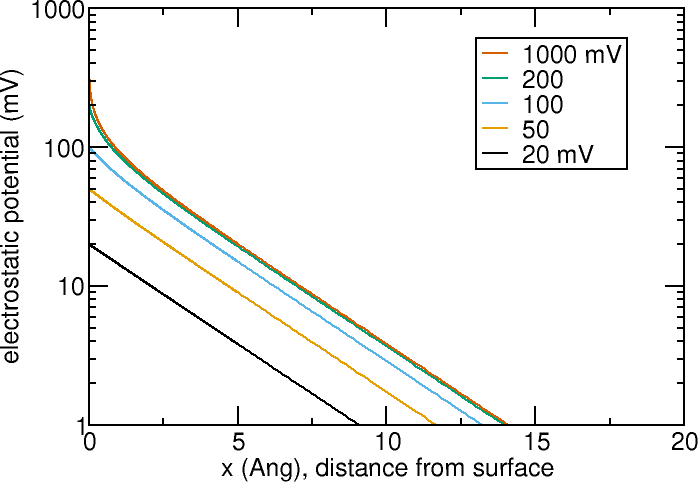
\includegraphics[width=0.45\linewidth]{counterion_potential.png}
(b)
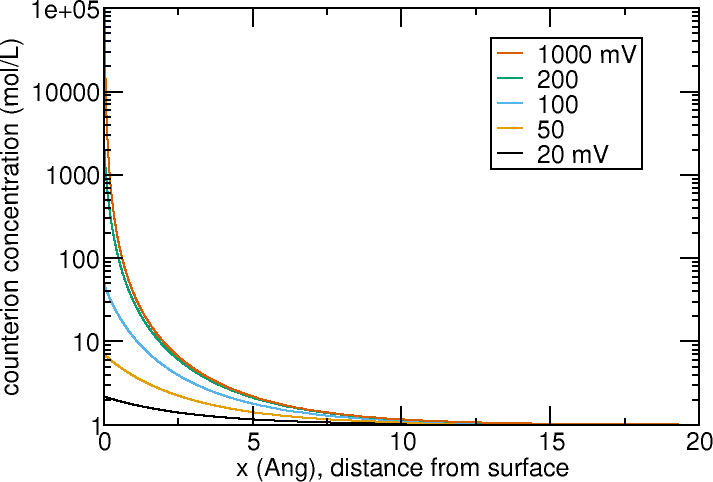
\includegraphics[width=0.45\linewidth]{counterion_logzero.png}
\caption{\label{fig_classical_PB}Solutions to the classical point
  charge Poisson-Boltzmann model of 1M NaCl electrolyte solution,
  shown as profiles along $x$, the perpendicular distance from an
  electrode surface (a) Electrostatic potential. (b) Counterion
  (\ce{Cl-}) concentration. }
\end{figure}

At still higher potentials the stability of simple log scaling with
respect to the coion must be considered. The coion, with same charge
as the electrostatic potential, is repelled from the electrode surface
with coion concentration trending towards zero at the electrode. At
sufficiently high potentials this generates values in the log-scaled
function that tend towards $-\infty$, which destabilises the numerical
solution. We therefore introduce a more complex log-scaling function,
\begin{equation}
Z_i(x) = \ln\left[c_i(x)/c_{i\infty}+1\right]/\ln 2 - 1
\label{log_zero}
\end{equation}
which keeps the scaled coion function constrained between -1 and 0
rather than $-\infty$ and 0. Since this scaling function addresses the
near-zero concentration of the coion, we call it ``log-zero'' scaling.

\section{Throttling algorithm}

Log-scaling of concentration functions makes a numerical solution to
the conventional Poisson-Boltzmann available at electrode potentials
up to 1.5V. Nevertheless \figref{fig_classical_PB}b demonstrates the
point charge catastrophe of the conventional model, with counterion
concentrations exceeding $10^{5}$ mol/L at the electrode
surface. Moreover, for general electrochemical applications it would
be desirable to be capable of obtaining solutions for electrode
potentials higher than 1.5V. To deal with the physical problem, we
introduce finite ion sizes with a steric force provided by the
Carnahan-Starling model, \eqnref{chem_pot_CS} (weak form
\eqnref{weak_CS}).  We apply ion volumes
$v_{\ce{Na}}=1.24 \text{\AA}^{3}$ per \ce{Na+} ion,
$v_{\ce{Cl}}=35.9 \text{\AA}^{3}$ per \ce{Cl-} ion (volumes taken from
quantum mechanical volumes of the ions' electron clouds
\cite{ParsonsNinham2009}).

The additional nonlinearity introduced by the Carnahan-Starling model,
where the chemical potential depends on the concentrations being
calculated, introduces a new challenge. The default nonlinear solver
in FEniCS assumes zero as an initial guess for the functions being
solved. But under the nonlinear conditions (with electrode potential
$>0.2$ V) where the Carnahan-Starling steric force is required, the
zero initial guess leads quickly to a diverging solution with infinite
residual. And yet a stable solution is accessible at lower values of
the boundary condition. We nudge the solver to a stable solution by
applying a throttling algorithm: reduce the boundary condition to a
small value for which a solution can be obtained, then incrementally
increase the boundary value back towards the target value, using the
previous found solution as an initial guess for the next
iteration. The approach is known to mathematicians as the homotopy
analysis method \cite{homotopy_analysis_Liao2012}, with our throttle
serving as a homotopy parameter applied to boundary conditions.
A flowchart for the algorithm is
shown in \figref{fig_throttling_algorithm}.

\begin{figure}
\centering
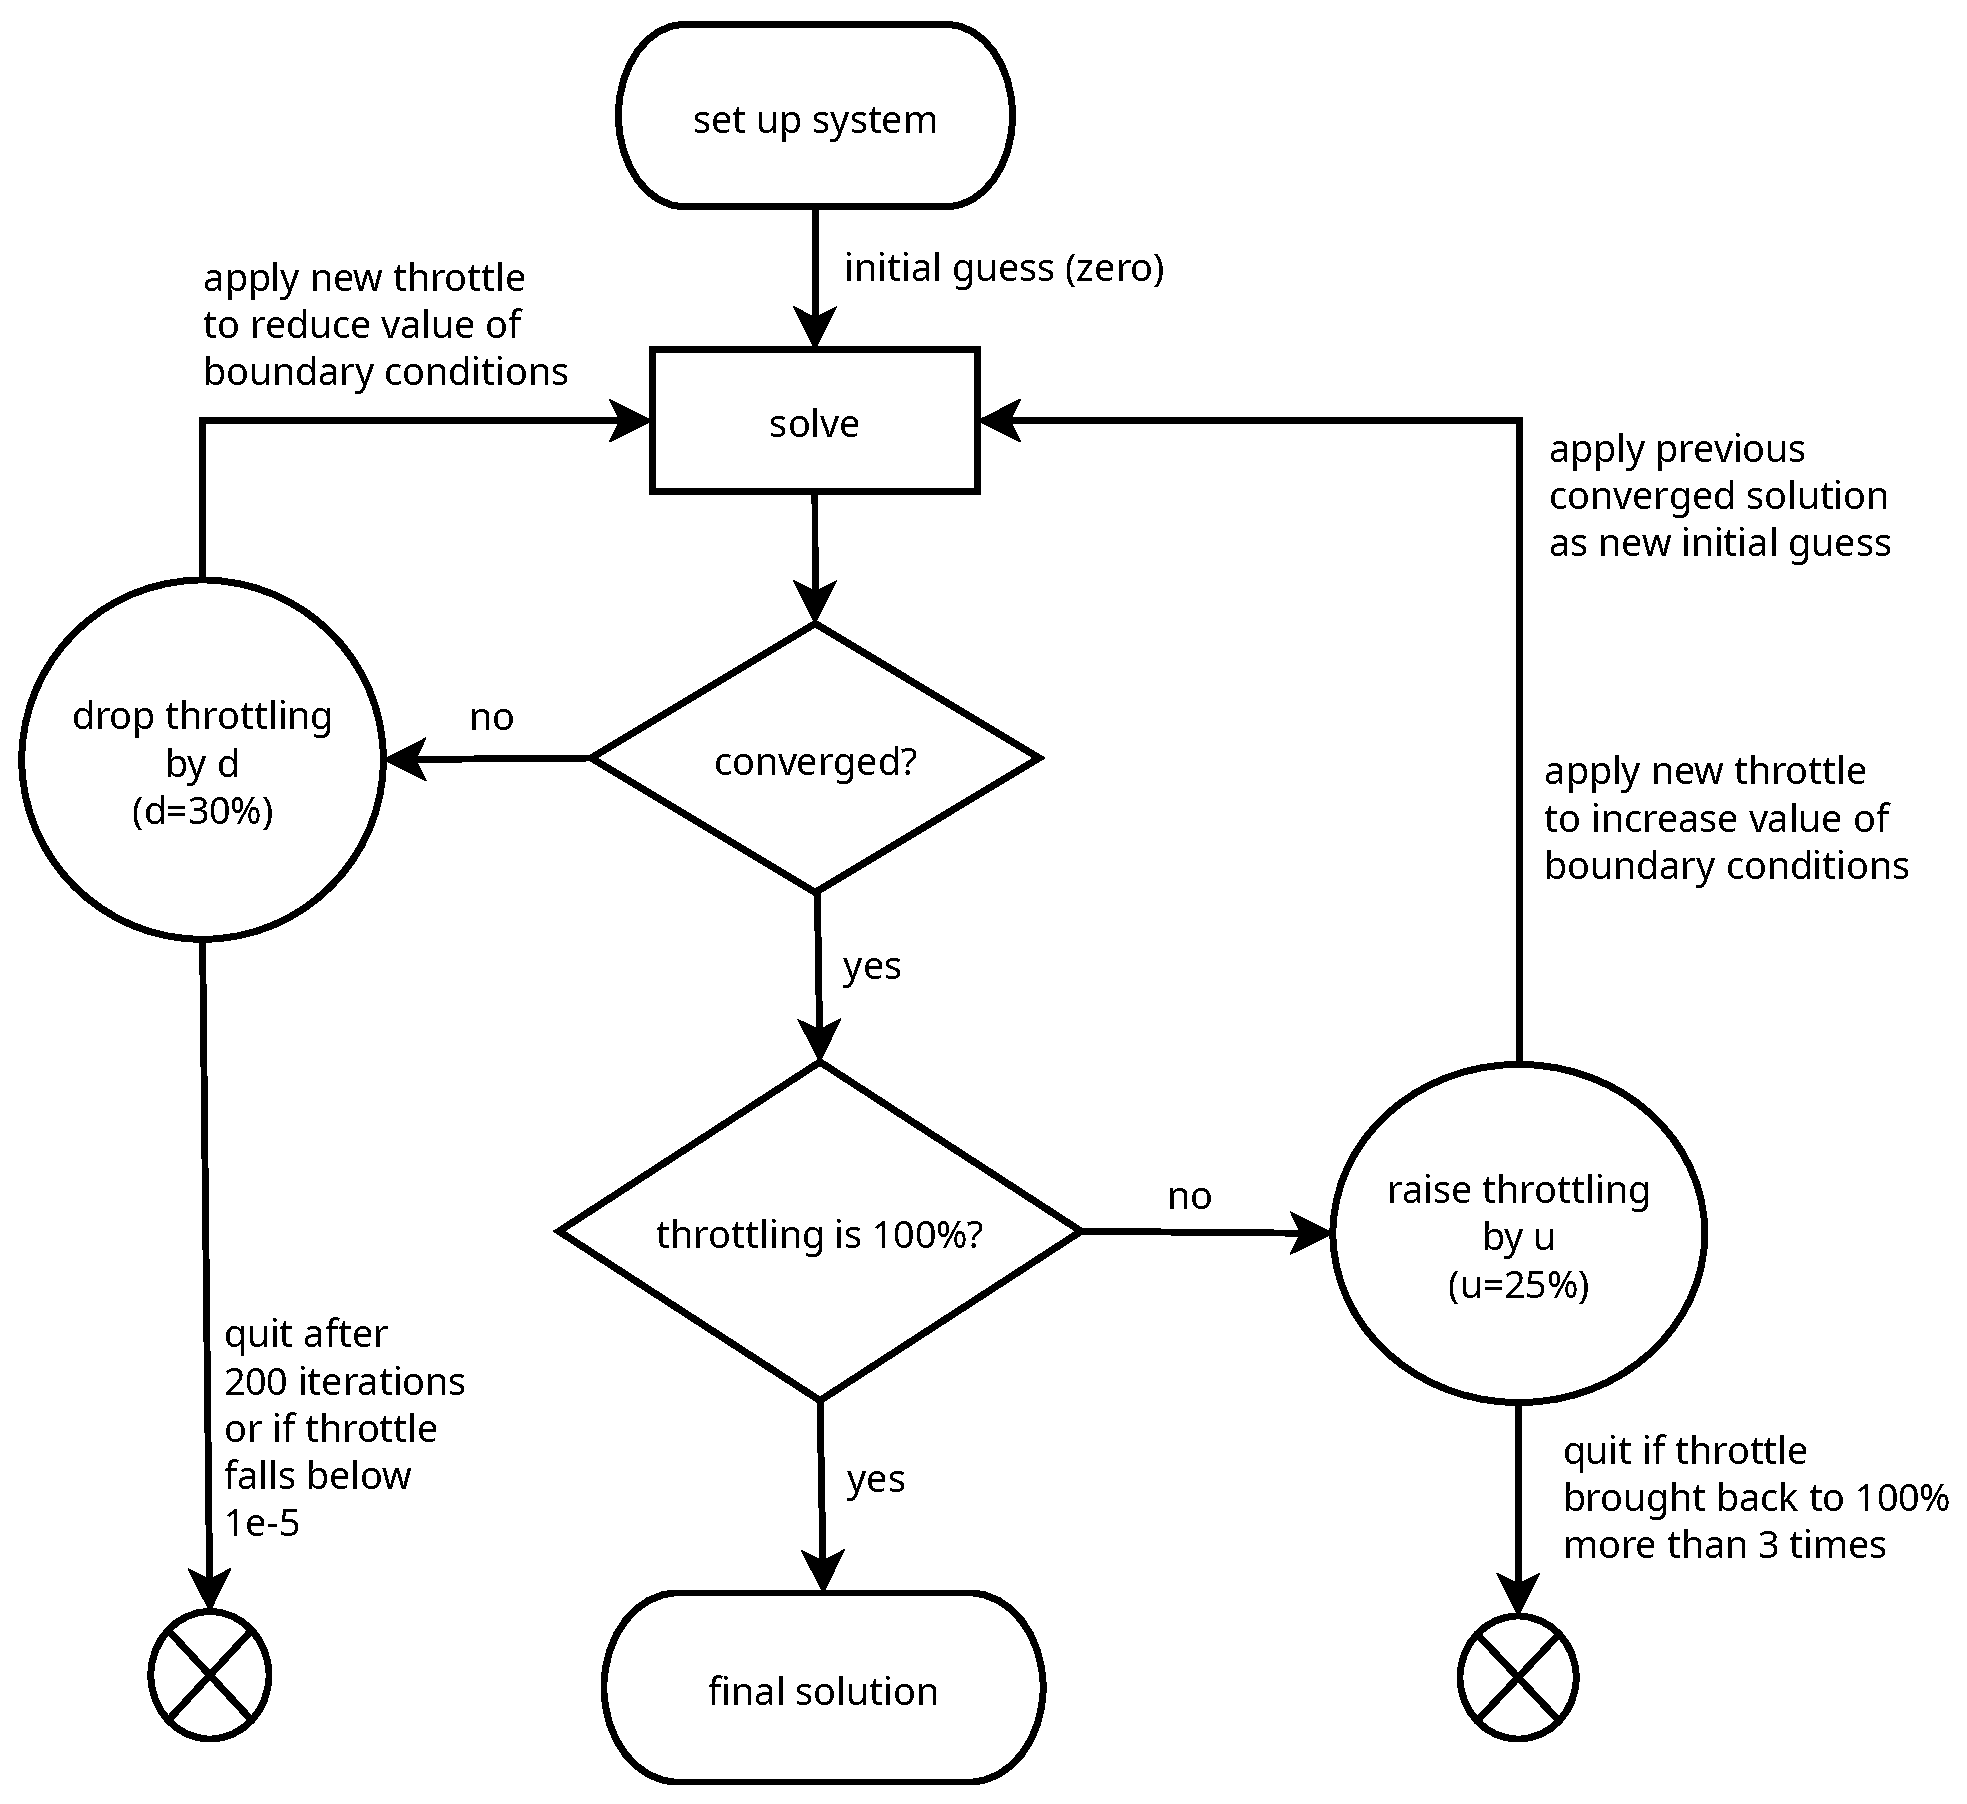
\includegraphics[width=0.8\linewidth]{throttling.eps}
\caption{\label{fig_throttling_algorithm}Flowchart for the throttling algorithm. }
\end{figure}

If the solver fails to converge, then reduce the throttle downwards to
a fraction $d$ of its previous value. The throttle is a multiplier
applied to the value of boundary conditions.  Once the boundary
condition is throttled enough to generate a converged solution, raise
the throttle upwards by an amount $u$, towards 100\% (set the throttle
to 100\% if the procedure would exceed it).  The values of $d$ and $u$
must find a balance between reaching 100\% throttle in as few
iterations as possible, while not collapsing back to non-converging
conditions when raising the throttle.  For potentials below 5V, we
find a drop level $d=75\%$ and a raise level $u=25\%$ with simple log
scaling of concentrations gives a reasonable balance between speed and
stability. If log-zero scaling is employed and the rise rate is
weakened to $u=10\%$, then electrode potentials of 20V can be
reached. With 5\% rising steps, 100V can be obtained. For a 1M
electrolyte, calculation at 240V would require such a small rise rate
that this algorithm becomes impractical.

If the throttling rates are not appropriately set, then the algorithm
may loop indefinitely between a converged solution at lower throttling
rate and non-convergence at a higher throttling rate. We therefore
halt after 200 throttle drops, or when the throttling rate drops below
$10^{-5}$, or when 100\% throttle is attempted more than 3 times.

The results of the throttling algorithm for an electrode charged to
10V, with Carnahan-Starling steric forces, is shown in
\figref{fig_results_throttling}. This solution was obtained with a
throttling rise rate of 10\% (0.1) and log-zero scaling of the
concentration functions
(\eqnref{log_zero}). \figref{fig_results_throttling} shows the onset
of a steric adsorption layer \cite{DagmawiParsons2022} with counterion
concentrations constrained below a concentration cap determined by the
ion size.

\begin{figure}
\centering
(a)
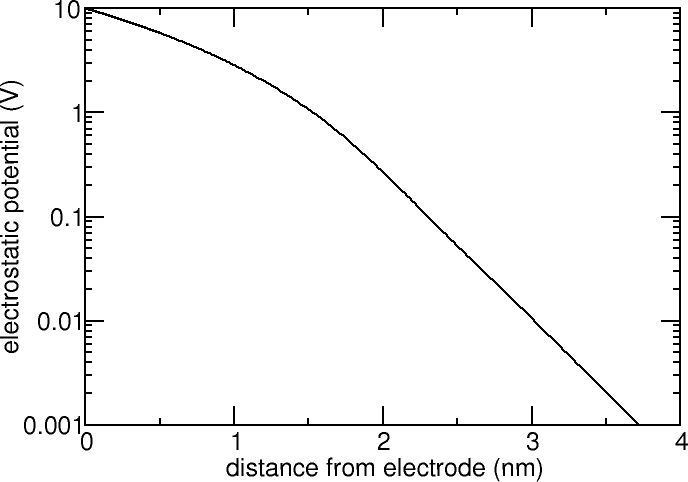
\includegraphics[width=0.4\linewidth]{steric_potential_10V.png}
(b)
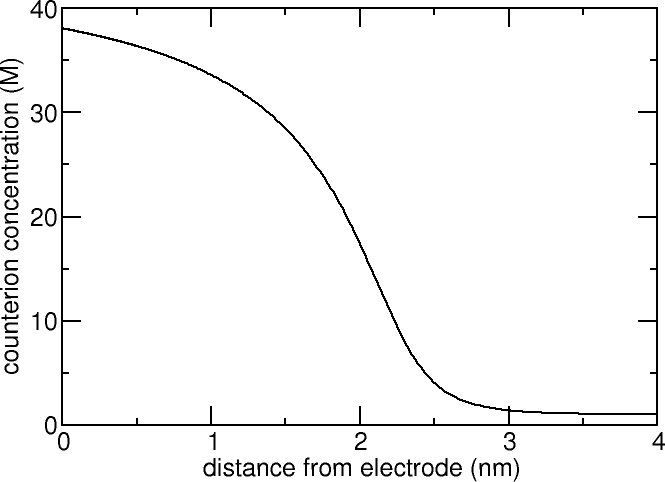
\includegraphics[width=0.4\linewidth]{steric_10V_counterion.png}
\caption{\label{fig_results_throttling}Solutions to the modified
  Poisson-Boltzmann model of a 1M NaCl electrolyte solution with
  Carnahan-Starling steric forces, shown as profiles along $x$, the
  perpendicular distance from a 5V electrode surface (a) Electrostatic
  potential. (b) Counterion (\ce{Cl-}) concentration. }
\end{figure}

\figref{fig_all_potential_high} presents algorithm conditions required
to obtains solutions (electrostatic potential profiles) up to
100V. Linear scaling (yellow region) is successful only for
$V<0.5$V. Log-scaling, \eqnref{log_scaling}, (purple region) with
throttling rise rate 25\% is successful up to 5V (purple
region). Log-zero scaling, \eqnref{log_zero}, with throttling rise
rate 10\% functions up to $V<20$V (blue region). Log-zero scaling with
5\% throttling rise rate can access up to $V<100$V (green region).

\begin{figure}
\centering
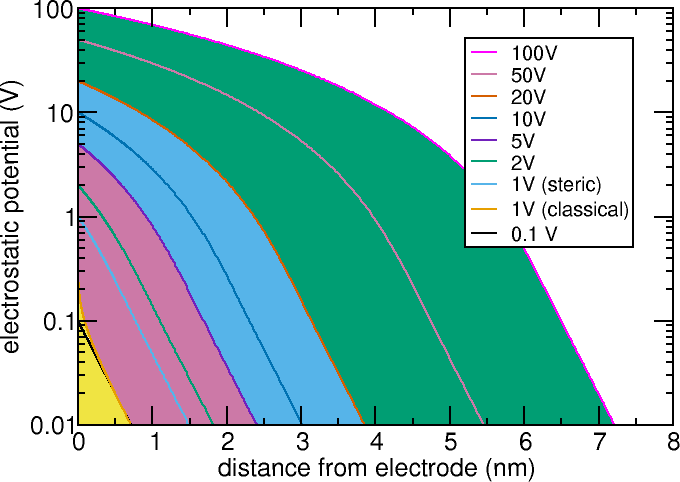
\includegraphics[width=0.9\linewidth]{counterion_potential_CS_bands.png}
\caption{\label{fig_all_potential_high} Algorithm conditions for
  electrostatic potential profiles with electrode potentials up to
  100V. Electrolyte is 1M NaCl. Linear scaling is functional for
  electrode potential $V<0.5$V (yellow region), log scaling (with
  steric forces) for $V<5$V with throttling rise rate 25\% (purple
  region), log-zero scaling with throttling rise rate 10\% for $V<20$V
  (blue region), and 5\% throttling rise rate for $V<100$V (green
  region).  }
\end{figure}

\section{Conclusion}

Modelling complex electrolyte solutions in electrochemical conditions
with electrode potentials 1V or greater requires both nontrivial
physics and nontrivial numerical algorithms. With respect to the
physics, aside from redox chemistry and electrolysis (not considered
here), the finite sizes of ions must be taken into consideration. With
respect to numerical convergence, we have proposed two
features. Firstly, we propose log-zero function scaling that accounts
not only for the heightened concentrations of counterions near an
electrode, but also the near-zero concentrations of coions. Secondly,
we propose a throttling algorithm that reduces boundary conditions
down to the linear regime where a solution is easily obtained, then
progressively propagating that solution by releasing the throttle
until the target boundary condition is obtained. The combination of
log-zero scaling and throttling enables calculations of electrolyte
solutions with electrode potentials up to 100V to be obtained. We
illustrated the throttling algorithm using Dirichlet boundary
conditions (electrode potentials), but the same principle applies
equally to Neumann or more complex boundary conditions.

\begin{acknowledgement}
  We acknowledge the award of CINECA support under the ISCRA
  initiative, for the availability of high-performance computing
  resources and support.
\end{acknowledgement}

\bibliographystyle{spbasic}
% Write the full path of your bibfile relative to book.tex
\bibliography{chapters/chp1/bibliography.bib}



%% Write the full path to the location of the graphics relative to book.tex
\graphicspath{{chapters/chp1/graphics/}}

\title{Function scaling and throttling for convergence control in highly nonlinear Poisson-Boltzmann electrolyte models.}
\titlerunning{Function Scaling and Convergence Throttling}

\author{D.~F.~Parsons, M.~Farci,  A.~Grigoras, Dagmawi Tadesse}
\authorrunning{Parsons et al.}

\institute{D.~F.~Parsons \email{drew.parsons@unica.it}
  \and M.~Farci \and A.~Grigoras
  \at University of Cagliari,
Department of Chemical and Geological Sciences \& CSGI,
Cittadella Universitaria, S.S. 554 bivio Sestu,
09042 Monserrato (CA), Italy
\and Dagmawi Tadesse
\at Murdoch University,
Discipline of Physics, Chemistry and Mathematics, 90 South St, Murdoch 6150, West Australia
}

\maketitle

\abstract{ The nonlinear Poisson-Boltzmann model of electrolyte
  solutions combines the Poisson equation for electrostatic potentials
  with a Boltzmann equilibrium of mobile ion concentrations. The
  Boltzmann equation $c(x) = c_0 \exp[-q\psi(x)/kT]$ is highly
  nonlinear once the electrostatic potential exceeds several thermal
  energy ($kT$) units (i.e.\ when $\psi>0.1$ V). This introduces two
  related numerical challenges. Firstly, suitable convergence criteria
  for the concentration functions becomes variable, depending on the
  boundary potential. Secondly a controlled initial guess must be
  provided must be provided to avoid the FEM calculation diverging to
  NaN. We resolve the first by logarithmic scaling of the
  concentration function, as suggested by the exponential nature of
  the Boltzmann equation.  However a nontrivial complex logarithmic
  form is required in order to allow for the near-zero concentrations
  of coions, which would trigger numerical divergence in a trivial
  $\ln[c(x)]$ scaled function. The second challenge is resolved by
  iteratively with a throttling algorithm that suppresses large
  boundary conditions down to the linear regime, which is then applied
  as an initial guess for the nonlinear regime. Our implementation
  allows for other nonelectrostatic molecular interactions important
  for modelling real chemical and electrochemical systems, in
  particular steric forces due to finite ions sizes, enabling
  computation of concentrated electrolytes with electrode potentials
  as high as 100V.  }

\section*{Introduction}

Continuum theory (mean field theory) has been an effective tool for
studying the behaviour of systems in electrolyte solutions. The
Poisson-Boltzmann (PB) model \cite{Wu2022} enables evaluation of ion
adsorption layers at surfaces together with the electric field that
surface charge and adsorbed ions generate. Its nonequilibrium
counterpart, the Poisson-Nernst-Planck model
\cite{LopezGarciaHornoGrosse2018} (also called drift-diffusion)
likewise enables simulation of systems under conditions of moving
current. The PB model underpins theory of colloidal stability,
enabling modelling of nanoparticle aggregation and surface forces. The
same theory can in principle be applied to model electrochemical
systems, including energy storage devices, batteries or
supercapacitors. But there is a crucial difference in the two classes
of application, which has a significant impact on the numerical
stability of the model.  The surface potentials (or zeta potentials)
of typical colloidal systems such as protein molecules or metal oxide
particles tends to be found in the range 5--50 mV, which is 0.2--2
$kT$ in thermal energy units (based on a thermal potential at $T=298$
K defined by $e\psi_{T} = kT$ (where $e$ is the elementary charge, $k$
is Boltzmann's constant, $T$ is temperature). Electrolytic energy
storage systems, by contrast, typically operate with electrode
potentials of the order of 1--5 V, that is 1000--5000 mV, or 40--200
$kT$.  The nonlinearity of the Poisson-Boltzmann model is highly
sensitive to energies exceeding one $kT$ unit, requiring particular
algorithms to enable numerical nonlinear convergence.  Our goal is to
set up the calculation to solve successfully over a broad range of
electrode potentials without requiring manual readjustment of
convergence parameters.  We identify two main steps, implemented via
finite element methods (using FEniCSx\cite{baratta2023dolfinx}): log-scaling of
ion concentration functions, and throttling of boundary
conditions. For context we also present a summary of the physics and
weak formulation defining the Poisson-Boltzmann model, including
finite ion size effects. For simplicity we omit redox phenomenon
(electrolysis of water would occur in real systems at high electrode
potentials).

\section{Weak formulation of the Poisson-Boltzmann model}

The energy functional for an electrolyte solution, determined by
electrostatic potential $\psi(x)$ and ion concentration profiles
$c_i(x)$, may be composed from various fundamental energy
contributions as
\begin{equation}
    \Omega[\psi, c_i] = \Omega_{el} + \Omega_{en} +  \Omega_{ex}
\end{equation}
$\Omega_{el}$ describes the direct energy of the electrostatic field generated by the electric charge of ions and surfaces, \cite{Jackson}
\begin{equation}
  \Omega_{el}  =\frac{1}{2} \int_{V}D \cdot E dx
  = -\frac{1}{2} \int_{V}D \cdot E dx + \sum_i \int_V z_i e c_i(x) \psi(x) dx
  + \int_{S} \sigma(s) \psi(s) ds
\end{equation}
where $E$ is the electric field $E=-\nabla\psi$ and $D$ is the
electric displacement $D=\varepsilon_0
\varepsilon(x)E$. $\varepsilon_0$ is the permittivity of the vacuum,
and $\varepsilon(x)$ is the (spatially varying) relative
permittivity. $z_i$ is the valency of ion $i$.  $\sigma(s)$ is the
surface charge density on boundary $S$.

$\Omega_{en}$ describes the ideal entropic energy of ions, treated as ideal (noninteracting) particles \cite{GrayStiles2018,DagmawiParsons2024},
\begin{equation}
    \Omega_{en} = kT \sum_{i} \int_{V} \left[ c_i(x) \ln \left(\frac{c_i(x)}{c_{i\infty}} \right) - c_{i}(x) + c_{i\infty} \right] dx 
\end{equation}
where $c_{i\infty}$ is the bulk concentration of ions. As a point of
physics it is important to note that the use of a fixed bulk
concentration means the system is controlled by the chemical potential
of ions with a variable number of ions in the domain $V$ of interest.
That is, the thermodynamic potential is a grand potential, not a
(Helmholtz) free energy (hence we write the energy as $\Omega$ rather
than $F$). A free energy formulation (with fixed number of ions) would
require use of a thermal de Broglie wavelength instead of
$c_{i\infty}$ \cite{GrayStiles2018}.

$\Omega_{el} + \Omega_{en}$ alone construct the conventional
Poisson-Boltzmann model. The term $\Omega_{ex}$ represents extra
contributions to the total energy functional that describes other
relevant physics, such as pH-dependent charge regulation
\cite{ParsonsSalis2019}, specific ion interactions
\cite{ParsonsCarucciSalis2022}, or steric forces due to finite ion
size \cite{LopezGarciaHornoGrosse2018}. We consider the latter in this
work.

The Poisson-Boltzmann model describes the system in equilibrium,
obtained by minimising the total grand potential with variation
$\delta\Omega=0$ with respect to $\psi$ and $c_i$. Variation with
respect to $\psi$ (with test function $p$) leads to a weak formulation
for the Poisson equation,
\begin{equation}
    0 = -\int_{V} \varepsilon_{0}\varepsilon(x) (\nabla\psi,\nabla p) dx + \sum_{i}z_i e \int_{V} c_{i}(x) p dx + \int_{S} \sigma(s) p ds  
    \label{weak_Poisson}
\end{equation}
for all $p$ in the relevant finite element space.  After additional
integration by parts, this weak formulation leads to the strong
formulation of the electrostatic Poisson equation,
$\nabla\cdot D = \sum_i z_i e c_{i}(x)$. Variation $\delta\Omega$ with
respect to each ion concentration profile $c_i$ (in turn, with test
function $b_i$), assuming linear variations with
$\ln(1+b_i/c_i)=b_i/c_i$, leads to the weak formulation of Boltzmann's
equation,
\begin{equation}
    0 = \int_{V}z_i e \psi(x) b_i dx
    + kT \int_{V} b_i \ln\left(\frac{c_i(x)}{c_{i\infty}}\right)dx
    \label{weak_Boltzmann}
\end{equation}
for all $b_i$. The strong form of the classical Boltzmann equation can then obtained, $c_i(x)=c_{i\infty}\exp(-z_i e \psi(x)/kT)$. 

It might be noted that in the classical Poisson-Boltzmann model, the
ion concentrations $c_i$ are determined completely by the
electrostatic potential with the Boltzmann equation in closed form, so
only the Poisson equation needs solving directly. However, the
physical problem with the classical model is evident in electrochemical
systems with electrode potential 1 V. A one volt potential is
equivalent to a thermal energy of $40 kT)$, for which the conventional
Boltzmann factor for a counterion is
$\exp(40)\approx 2.3 \times 10^{17}$.  That is, the surface counterion
concentration of a 1M electrolyte would exceed $10^{17}$ mol/L, which
is obviously unphysical.  We return the model back to physical
relevance by adding an extra steric energy term $\Omega_{ex}$ with
corresponding excess chemical potential per ion $\mu_{i}^{ex}$, for
which the modified Boltzmann equation is
\begin{equation}
    c_i(x)=c_{i\infty}\exp\left[(-(z_i e \psi(x) + \mu_i^{ex}(x)-\mu_{i\infty}^{ex})/kT\right]
    \label{general_Boltzmann}
\end{equation}
$\mu_{i\infty}$ refers to the (fixed) excess chemical potential of the ion in bulk solution.
The steric model we employ is the Carnahan-Starling model \cite{CarnahanStarling1969} with grand potential
\begin{equation}
    \Omega_{ex} = \sum_{i} \int_{V} c_{i}(x) \left[ kT
    \frac{4\phi - 3\phi^2}{(1-\phi)^2}
    -  \mu_{\infty}
    \right]dx
\end{equation}
and weak formulation
\begin{equation}
    0 = \int_{V} (\mu_i^{ex}-\mu_{i\infty}^{ex}) b_i
    \label{weak_CS}
\end{equation}
for all $b_i$, which adds to \eqnref{weak_Boltzmann}, the weak
formulation for the Boltzmann equation, together generating the strong
formulation of \eqnref{general_Boltzmann}, the modified Boltzmann
equation.  Here we have introduced from the excess chemical potential
per ion for the Carnahan-Starling model,
\begin{equation}
    \mu_{i}^{ex} = kT \frac{\phi(8-9\phi+3\phi^2)}{(1-\phi)^3}
    \label{chem_pot_CS}
\end{equation}
Crucially, $\phi$ is the \emph{total} ion volume fraction defined by
$\phi=\sum_i c_i v_i$ where $v_i$ is the intrinsic molar volume per
ion $i$. Hence the CS excess chemical potential is defined identically
for all ions. To derive the weak formulation in \eqnref{weak_CS}, we
applied an homogenised component approximation that assigns common
volumes when introducing the test function $b_i$ (which is the
variation $\delta c_i$), such that $\delta\phi=v_j \delta c_i$ rather
than $v_i \delta c_i$. This approximation is required since the CS
model was formulated for single component systems. The more complex
multicomponent BMCSL model would enable ion specific chemical
potentials \cite{MansooriCarnahanStarlingLeland1971}, removing the
need for this approximation.  $\phi_{\infty}$, $\mu_{i\infty}^{ex}$
are the bulk total volume fraction and excess chemical potential
defined by bulk concentrations $c_{i\infty}$. With this term, the
Boltzmann equation is transcendental in $c_i$, precluding a closed
expression determining ion concentrations, which must therefore be
explicitly numerically solved alongside potential $\psi$. In this
paper we address strategies for managing the strong nonlinearity in
the system introduced by this term alongside large values of the
potential. Note that $c_i$ must also be solved explicitly in the case
of time-dependent nonequilibrium Poisson-Nernst-Planck systems where
ion concentrations are not in equilibrium and determined by a
continuity equation rather than a Boltzmann equation.

\section{Function scaling}
We constructed a finite element implementation of the weak
formulation(\eqnref{weak_Poisson} and \ref{weak_Boltzmann} (and
\eqnref{weak_CS}) in FEniCS-X \cite{baratta2023dolfinx}, using continuous
Lagrange elements with polynomial order 2.  The electrolyte solution
is taken as NaCl with bulk concentration 1 mol/L.  To illustrate
general issues of nonlinear convergence, we calculate the
electrostatic and ion concentration profiles of ion adsorbed at a
single flat electrode surface along the direction perpendicular to the
surface, with the electrode boundary at $x=0$.  The electrode
potential is controlled (Dirichlet boundary condition), and bulk
solution represented by a zero Neumann condition ("zero electric
field") at a distance of 30 Debye lengths (at $x=9.1$ nm, for the 1M
electrolyte). Nonlinear solutions are computed using FEniCS-X's
NonlinearProblem with a standard NewtonSolver. Convergence criterion
is set to FEniCS-X's default "incremental" method with absolute
tolerance $10^{-5}$.

We must consider scaling of the concentration functions $c_i(x)$. We
already noted that the counterion concentration becomes unphysically
large in the conventional Poisson-Boltzmann model due to nonlinear
exponentiation of the electrostatic potentials exceeding 0.1--0.2 V in
the Boltzmann equation. Trivial scaling may be introduced by solving
the concentration function scaled against the bulk concentration. But
with a convergence criterion of the nonlinear catastrophe is reached
numerically above 0.5 V. Already at 0.6 V, the conventional
calculation with simple scaling is unable to reduce the residual below
the required $10^{-5}$. While it would be possible to relax the
convergence tolerance to obtain a reasonable solution, our aim is to
obtain a robust general solver not requiring close manipulation of
convergence criteria. For instance, one application is modelling the
cyclic voltammetry curve of an electrode which require calculations
over a potential window as wide as $-5$ to 5 V.

The challenge arises due to the extreme magnitudes of the counterion
concentration at the electrode surface. The weak formulation for the
Boltzmann equation in \eqnref{weak_Boltzmann} suggests a solution:
solve for the concentration function in log-form,
\begin{equation}
C_{i}(x) = \ln[ c_{i}(x) / c_{i\infty}]
\label{log_scaling}
\end{equation}
rather than the concentration function $c_{i}(x)$ directly. Log
scaling extends the solvability of the conventional Poisson-Boltzmann
model up to electrode potentials as high as 1.5 V. Solutions for the
electrostatic potential and counterion concentration profile are shown
in \figref{fig_classical_PB}. Shown on a log scale, strong
nonlinearity in the PB system becomes apparent in the bend in the
electrostatic potential (\figref{fig_classical_PB}a) close to the
surface where $x<2$\AA for electrode potentials $> 0.2$ V.


\begin{figure}
\centering
(a)
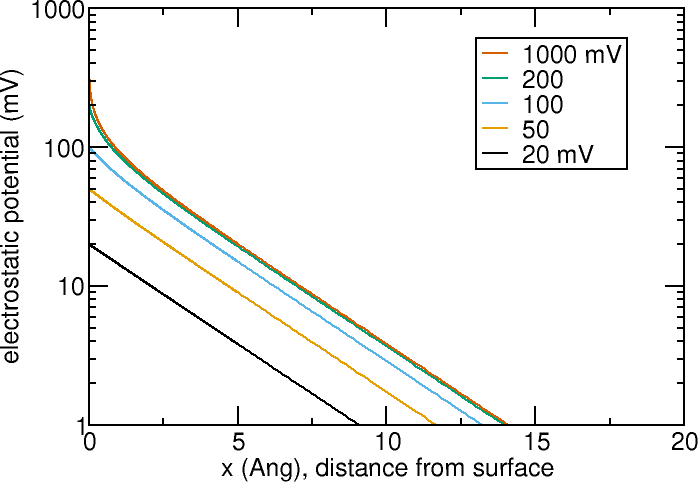
\includegraphics[width=0.45\linewidth]{counterion_potential.png}
(b)
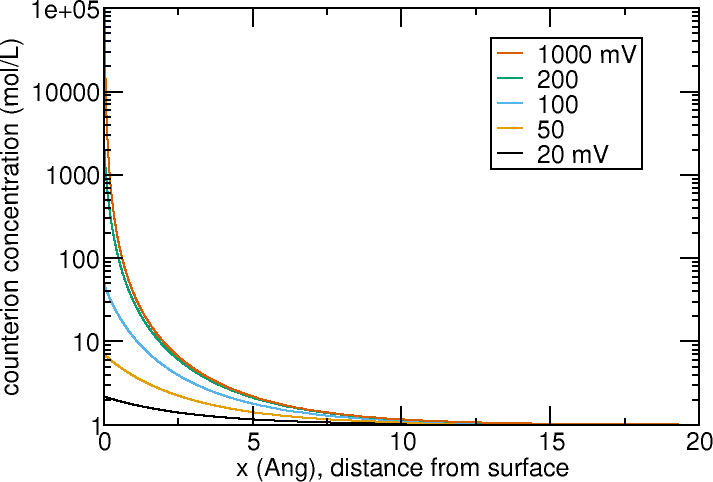
\includegraphics[width=0.45\linewidth]{counterion_logzero.png}
\caption{\label{fig_classical_PB}Solutions to the classical point
  charge Poisson-Boltzmann model of 1M NaCl electrolyte solution,
  shown as profiles along $x$, the perpendicular distance from an
  electrode surface (a) Electrostatic potential. (b) Counterion
  (\ce{Cl-}) concentration. }
\end{figure}

At still higher potentials the stability of simple log scaling with
respect to the coion must be considered. The coion, with same charge
as the electrostatic potential, is repelled from the electrode surface
with coion concentration trending towards zero at the electrode. At
sufficiently high potentials this generates values in the log-scaled
function that tend towards $-\infty$, which destabilises the numerical
solution. We therefore introduce a more complex log-scaling function,
\begin{equation}
Z_i(x) = \ln\left[c_i(x)/c_{i\infty}+1\right]/\ln 2 - 1
\label{log_zero}
\end{equation}
which keeps the scaled coion function constrained between -1 and 0
rather than $-\infty$ and 0. Since this scaling function addresses the
near-zero concentration of the coion, we call it ``log-zero'' scaling.

\section{Throttling algorithm}

Log-scaling of concentration functions makes a numerical solution to
the conventional Poisson-Boltzmann available at electrode potentials
up to 1.5V. Nevertheless \figref{fig_classical_PB}b demonstrates the
point charge catastrophe of the conventional model, with counterion
concentrations exceeding $10^{5}$ mol/L at the electrode
surface. Moreover, for general electrochemical applications it would
be desirable to be capable of obtaining solutions for electrode
potentials higher than 1.5V. To deal with the physical problem, we
introduce finite ion sizes with a steric force provided by the
Carnahan-Starling model, \eqnref{chem_pot_CS} (weak form
\eqnref{weak_CS}).  We apply ion volumes
$v_{\ce{Na}}=1.24 \text{\AA}^{3}$ per \ce{Na+} ion,
$v_{\ce{Cl}}=35.9 \text{\AA}^{3}$ per \ce{Cl-} ion (volumes taken from
quantum mechanical volumes of the ions' electron clouds
\cite{ParsonsNinham2009}).

The additional nonlinearity introduced by the Carnahan-Starling model,
where the chemical potential depends on the concentrations being
calculated, introduces a new challenge. The default nonlinear solver
in FEniCS assumes zero as an initial guess for the functions being
solved. But under the nonlinear conditions (with electrode potential
$>0.2$ V) where the Carnahan-Starling steric force is required, the
zero initial guess leads quickly to a diverging solution with infinite
residual. And yet a stable solution is accessible at lower values of
the boundary condition. We nudge the solver to a stable solution by
applying a throttling algorithm: reduce the boundary condition to a
small value for which a solution can be obtained, then incrementally
increase the boundary value back towards the target value, using the
previous found solution as an initial guess for the next
iteration. The approach is known to mathematicians as the homotopy
analysis method \cite{homotopy_analysis_Liao2012}, with our throttle
serving as a homotopy parameter applied to boundary conditions.
A flowchart for the algorithm is
shown in \figref{fig_throttling_algorithm}.

\begin{figure}
\centering
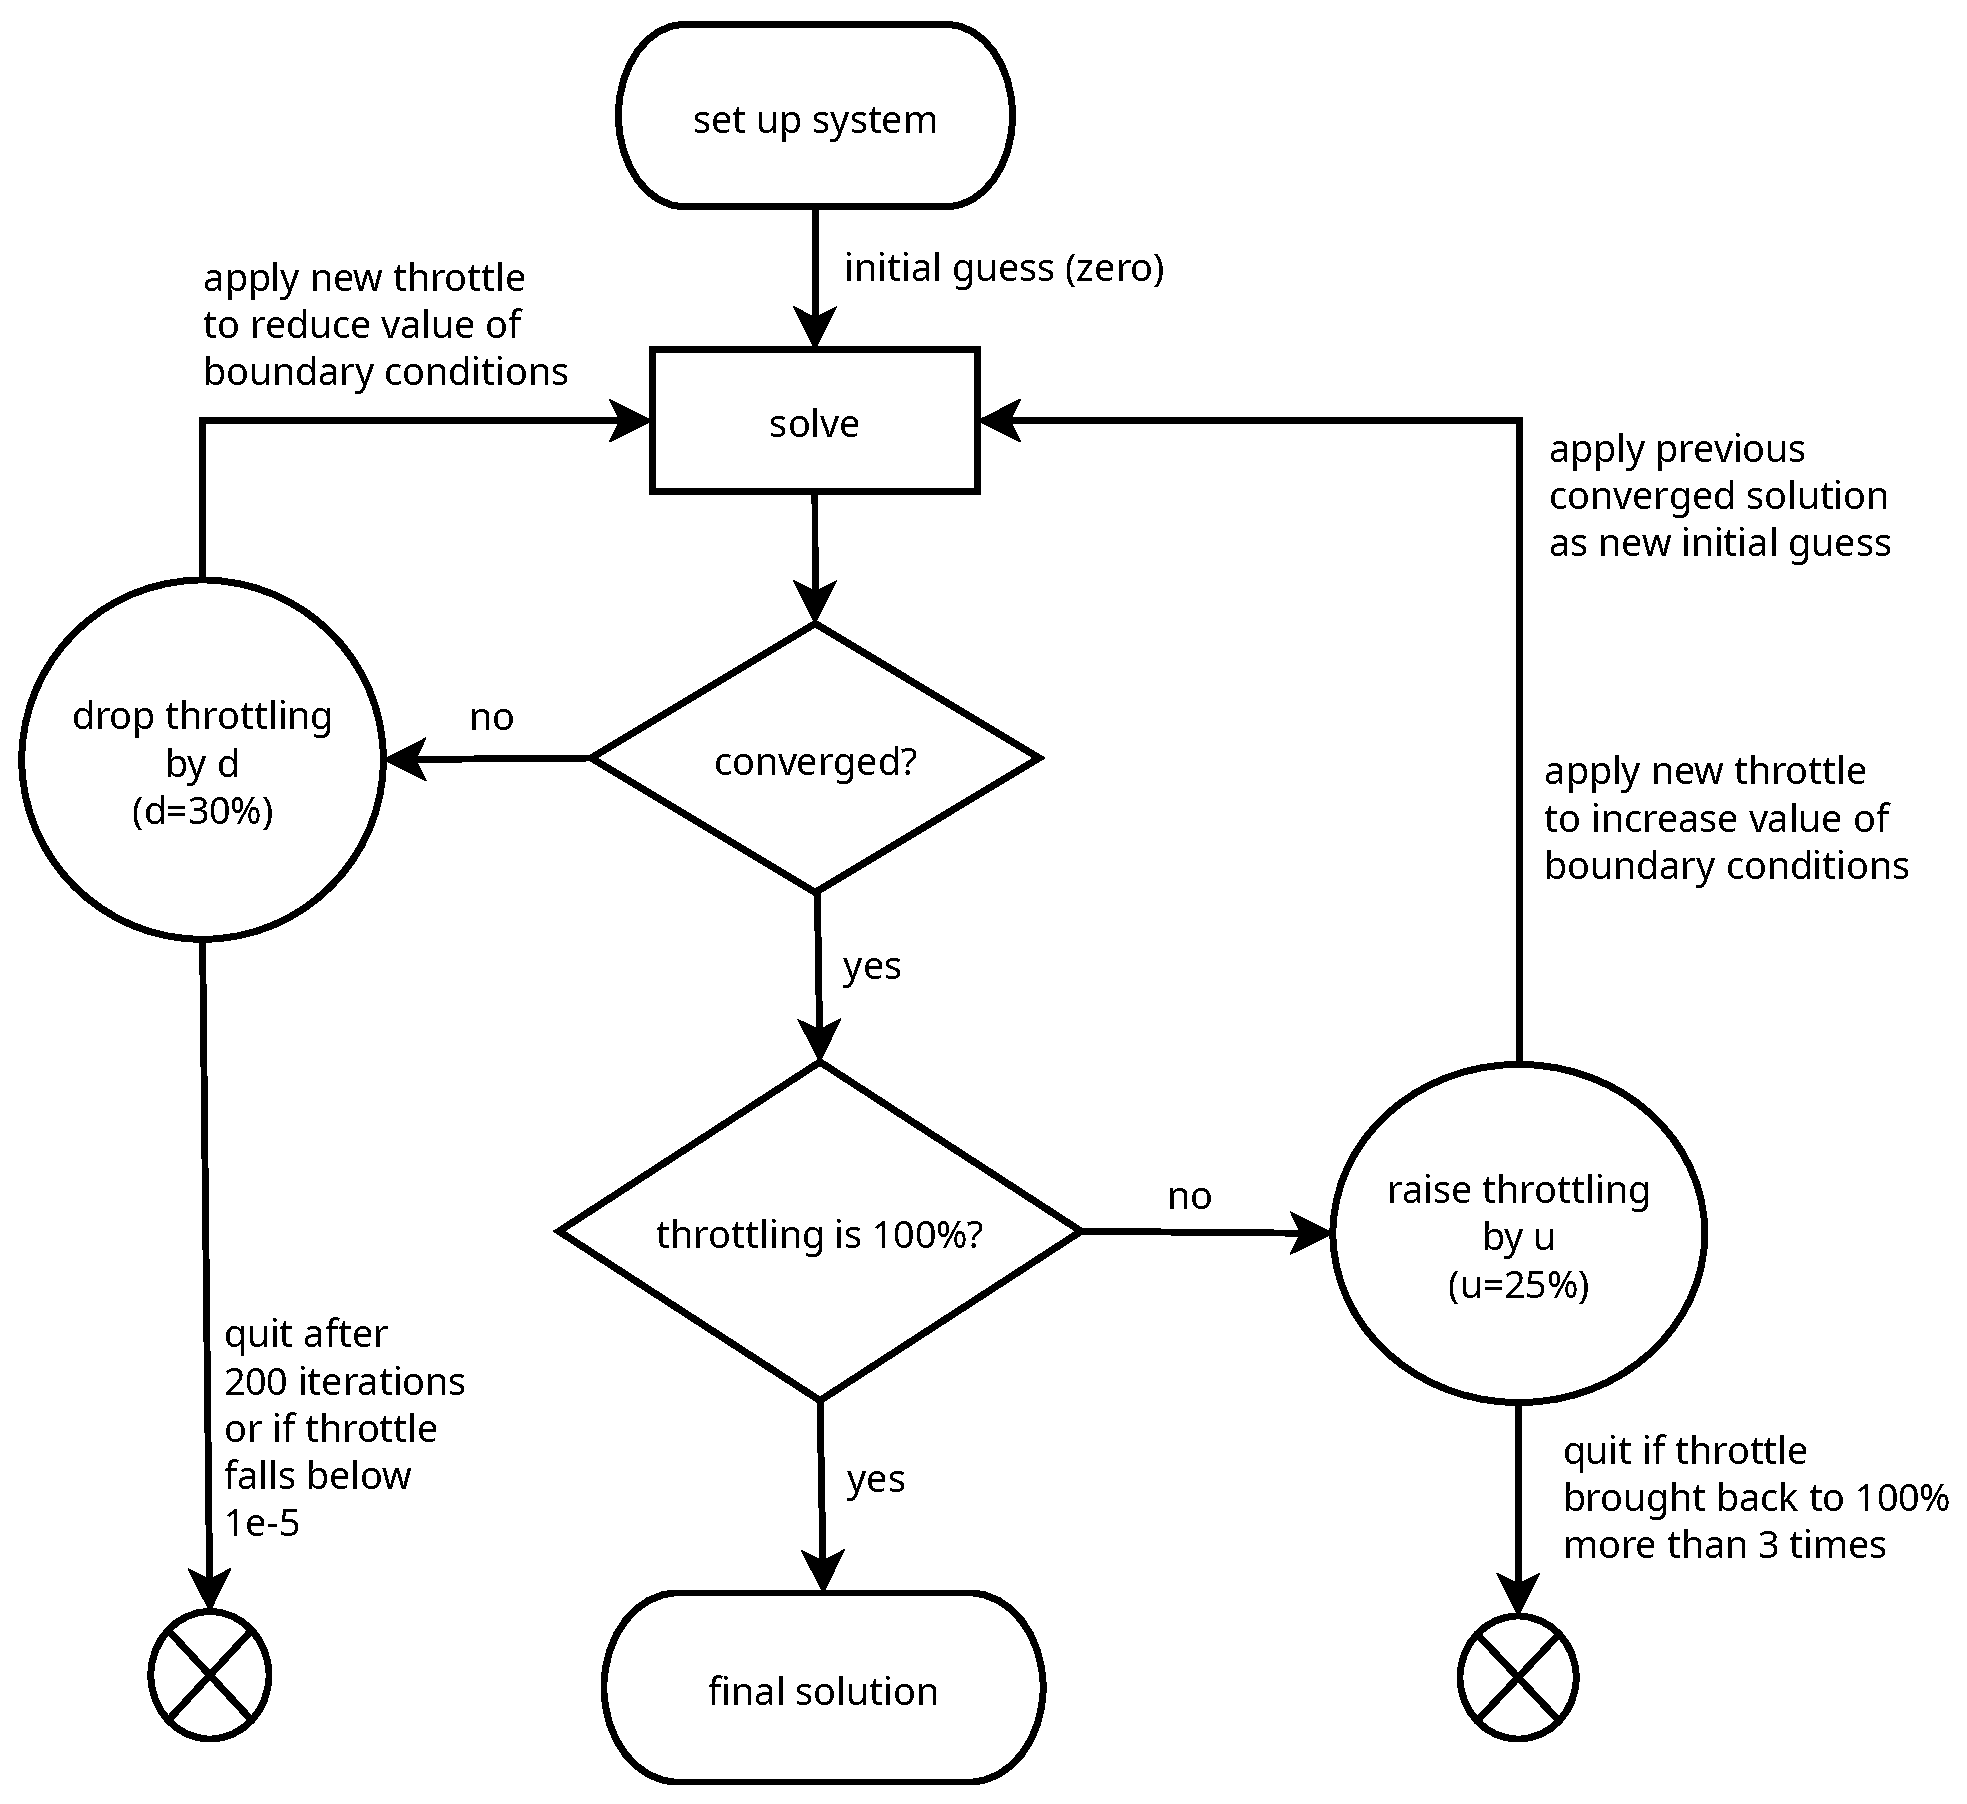
\includegraphics[width=0.8\linewidth]{throttling.eps}
\caption{\label{fig_throttling_algorithm}Flowchart for the throttling algorithm. }
\end{figure}

If the solver fails to converge, then reduce the throttle downwards to
a fraction $d$ of its previous value. The throttle is a multiplier
applied to the value of boundary conditions.  Once the boundary
condition is throttled enough to generate a converged solution, raise
the throttle upwards by an amount $u$, towards 100\% (set the throttle
to 100\% if the procedure would exceed it).  The values of $d$ and $u$
must find a balance between reaching 100\% throttle in as few
iterations as possible, while not collapsing back to non-converging
conditions when raising the throttle.  For potentials below 5V, we
find a drop level $d=75\%$ and a raise level $u=25\%$ with simple log
scaling of concentrations gives a reasonable balance between speed and
stability. If log-zero scaling is employed and the rise rate is
weakened to $u=10\%$, then electrode potentials of 20V can be
reached. With 5\% rising steps, 100V can be obtained. For a 1M
electrolyte, calculation at 240V would require such a small rise rate
that this algorithm becomes impractical.

If the throttling rates are not appropriately set, then the algorithm
may loop indefinitely between a converged solution at lower throttling
rate and non-convergence at a higher throttling rate. We therefore
halt after 200 throttle drops, or when the throttling rate drops below
$10^{-5}$, or when 100\% throttle is attempted more than 3 times.

The results of the throttling algorithm for an electrode charged to
10V, with Carnahan-Starling steric forces, is shown in
\figref{fig_results_throttling}. This solution was obtained with a
throttling rise rate of 10\% (0.1) and log-zero scaling of the
concentration functions
(\eqnref{log_zero}). \figref{fig_results_throttling} shows the onset
of a steric adsorption layer \cite{DagmawiParsons2022} with counterion
concentrations constrained below a concentration cap determined by the
ion size.

\begin{figure}
\centering
(a)
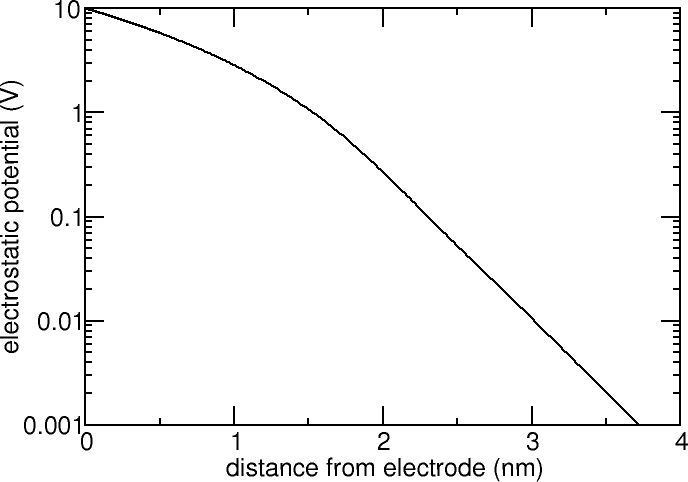
\includegraphics[width=0.4\linewidth]{steric_potential_10V.png}
(b)
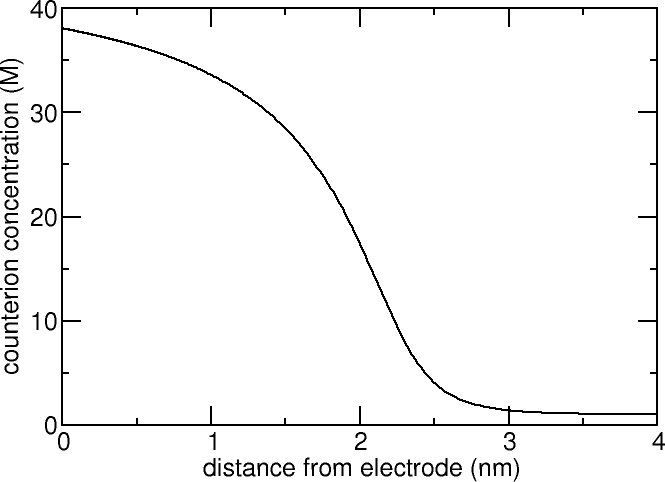
\includegraphics[width=0.4\linewidth]{steric_10V_counterion.png}
\caption{\label{fig_results_throttling}Solutions to the modified
  Poisson-Boltzmann model of a 1M NaCl electrolyte solution with
  Carnahan-Starling steric forces, shown as profiles along $x$, the
  perpendicular distance from a 5V electrode surface (a) Electrostatic
  potential. (b) Counterion (\ce{Cl-}) concentration. }
\end{figure}

\figref{fig_all_potential_high} presents algorithm conditions required
to obtains solutions (electrostatic potential profiles) up to
100V. Linear scaling (yellow region) is successful only for
$V<0.5$V. Log-scaling, \eqnref{log_scaling}, (purple region) with
throttling rise rate 25\% is successful up to 5V (purple
region). Log-zero scaling, \eqnref{log_zero}, with throttling rise
rate 10\% functions up to $V<20$V (blue region). Log-zero scaling with
5\% throttling rise rate can access up to $V<100$V (green region).

\begin{figure}
\centering
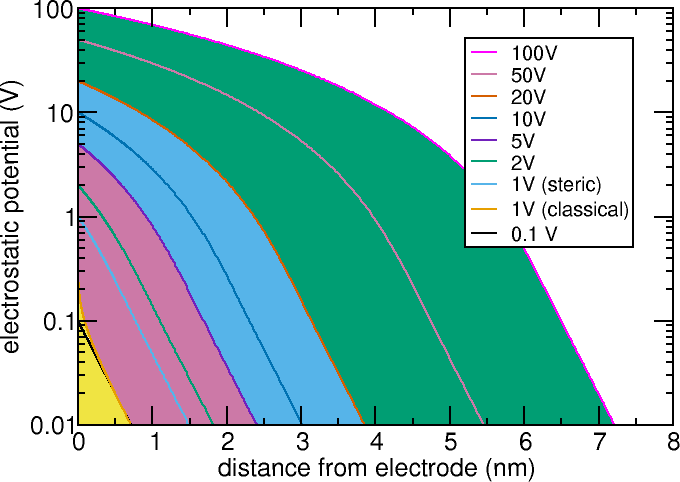
\includegraphics[width=0.9\linewidth]{counterion_potential_CS_bands.png}
\caption{\label{fig_all_potential_high} Algorithm conditions for
  electrostatic potential profiles with electrode potentials up to
  100V. Electrolyte is 1M NaCl. Linear scaling is functional for
  electrode potential $V<0.5$V (yellow region), log scaling (with
  steric forces) for $V<5$V with throttling rise rate 25\% (purple
  region), log-zero scaling with throttling rise rate 10\% for $V<20$V
  (blue region), and 5\% throttling rise rate for $V<100$V (green
  region).  }
\end{figure}

\section{Conclusion}

Modelling complex electrolyte solutions in electrochemical conditions
with electrode potentials 1V or greater requires both nontrivial
physics and nontrivial numerical algorithms. With respect to the
physics, aside from redox chemistry and electrolysis (not considered
here), the finite sizes of ions must be taken into consideration. With
respect to numerical convergence, we have proposed two
features. Firstly, we propose log-zero function scaling that accounts
not only for the heightened concentrations of counterions near an
electrode, but also the near-zero concentrations of coions. Secondly,
we propose a throttling algorithm that reduces boundary conditions
down to the linear regime where a solution is easily obtained, then
progressively propagating that solution by releasing the throttle
until the target boundary condition is obtained. The combination of
log-zero scaling and throttling enables calculations of electrolyte
solutions with electrode potentials up to 100V to be obtained. We
illustrated the throttling algorithm using Dirichlet boundary
conditions (electrode potentials), but the same principle applies
equally to Neumann or more complex boundary conditions.

\begin{acknowledgement}
  We acknowledge the award of CINECA support under the ISCRA
  initiative, for the availability of high-performance computing
  resources and support.
\end{acknowledgement}

\bibliographystyle{spbasic}
% Write the full path of your bibfile relative to book.tex
\bibliography{chapters/chp1/bibliography.bib}





\backmatter%%%%%%%%%%%%%%%%%%%%%%%%%%%%%%%%%%%%%%%%%%%%%%%%%%%%%%%
\appendix
%%%%%%%%%%%%%%%%%%%%%% appendix.tex %%%%%%%%%%%%%%%%%%%%%%%%%%%%%%%%%
%
% sample appendix
%
% Use this file as a template for your own input.
%
%%%%%%%%%%%%%%%%%%%%%%%% Springer-Verlag %%%%%%%%%%%%%%%%%%%%%%%%%%

\chapter{Chapter Heading}
\label{introA} % Always give a unique label
% use \chaptermark{}
% to alter or adjust the chapter heading in the running head

Use the template \emph{appendix.tex} together with the document class SVMono (monograph-type books) or SVMult (edited books) to style appendix of your book.


\section{Section Heading}
\label{sec:A1}
% Always give a unique label
% and use \ref{<label>} for cross-references
% and \cite{<label>} for bibliographic references
% use \sectionmark{}
% to alter or adjust the section heading in the running head
Instead of simply listing headings of different levels we recommend to let every heading be followed by at least a short passage of text. Further on please use the \LaTeX\ automatism for all your cross-references and citations.


\subsection{Subsection Heading}
\label{sec:A2}
Instead of simply listing headings of different levels we recommend to let every heading be followed by at least a short passage of text. Further on please use the \LaTeX\ automatism for all your cross-references and citations as has already been described in Sect.~\ref{sec:A1}.

For multiline equations we recommend to use the \verb|eqnarray| environment.
\begin{eqnarray}
\vec{a}\times\vec{b}=\vec{c} \nonumber\\
\vec{a}\times\vec{b}=\vec{c}
\label{eq:A01}
\end{eqnarray}

\subsubsection{Subsubsection Heading}
Instead of simply listing headings of different levels we recommend to let every heading be followed by at least a short passage of text. Further on please use the \LaTeX\ automatism for all your cross-references and citations as has already been described in Sect.~\ref{sec:A2}.

Please note that the first line of text that follows a heading is not indented, whereas the first lines of all subsequent paragraphs are.

% For figures use
%
\begin{figure}[t]
\sidecaption[t]
% Use the relevant command for your figure-insertion program
% to insert the figure file.
% For example, with the graphicx style use
\includegraphics[scale=.65]{figure}
%
% If no graphics program available, insert a blank space i.e. use
%\picplace{5cm}{2cm} % Give the correct figure height and width in cm
%
\caption{Please write your figure caption here}
\label{fig:A1}       % Give a unique label
\end{figure}

% For tables use
%
\begin{table}
\caption{Please write your table caption here}
\label{tab:A1}       % Give a unique label
%
% Follow this input for your own table layout
%
\begin{tabular}{p{2cm}p{2.4cm}p{2cm}p{4.9cm}}
\hline\noalign{\smallskip}
Classes & Subclass & Length & Action Mechanism  \\
\noalign{\smallskip}\hline\noalign{\smallskip}
Translation & mRNA$^a$  & 22 (19--25) & Translation repression, mRNA cleavage\\
Translation & mRNA cleavage & 21 & mRNA cleavage\\
Translation & mRNA  & 21--22 & mRNA cleavage\\
Translation & mRNA  & 24--26 & Histone and DNA Modification\\
\noalign{\smallskip}\hline\noalign{\smallskip}
\end{tabular}
$^a$ Table foot note (with superscript)
\end{table}
%

%%%%%%%%%%%%%%%%%%%%%%acronym.tex%%%%%%%%%%%%%%%%%%%%%%%%%%%%%%%%%%%%%%%%%
% sample list of acronyms
%
% Use this file as a template for your own input.
%
%%%%%%%%%%%%%%%%%%%%%%%% Springer Nature%%%%%%%%%%%%%%%%%%%%%%%%%%

\Extrachap{Glossary}


Use the template \emph{glossary.tex} together with the Springer Nature document class SVMono (monograph-type books) or SVMult (edited books) to style your glossary\index{glossary} in the Springer Nature layout.


\runinhead{glossary term} Write here the description of the glossary term. Write here the description of the glossary term. Write here the description of the glossary term.

\runinhead{glossary term} Write here the description of the glossary term. Write here the description of the glossary term. Write here the description of the glossary term.

\runinhead{glossary term} Write here the description of the glossary term. Write here the description of the glossary term. Write here the description of the glossary term.

\runinhead{glossary term} Write here the description of the glossary term. Write here the description of the glossary term. Write here the description of the glossary term.

\runinhead{glossary term} Write here the description of the glossary term. Write here the description of the glossary term. Write here the description of the glossary term.
\printindex

%%%%%%%%%%%%%%%%%%%%%%%%%%%%%%%%%%%%%%%%%%%%%%%%%%%%%%%%%%%%%%%%%%%%%%

\end{document}

